\documentclass[crop=false,class=book,oneside]{standalone}
%----------------------------Preamble-------------------------------%
%---------------------------Packages----------------------------%
\usepackage{geometry}
\geometry{b5paper, margin=1.0in}
\usepackage[T1]{fontenc}
\usepackage{graphicx, float}            % Graphics/Images.
\usepackage{natbib}                     % For bibliographies.
\bibliographystyle{agsm}                % Bibliography style.
\usepackage[french, english]{babel}     % Language typesetting.
\usepackage[dvipsnames]{xcolor}         % Color names.
\usepackage{listings}                   % Verbatim-Like Tools.
\usepackage{mathtools, esint, mathrsfs} % amsmath and integrals.
\usepackage{amsthm, amsfonts, amssymb}  % Fonts and theorems.
\usepackage{tcolorbox}                  % Frames around theorems.
\usepackage{upgreek}                    % Non-Italic Greek.
\usepackage{fmtcount, etoolbox}         % For the \book{} command.
\usepackage[newparttoc]{titlesec}       % Formatting chapter, etc.
\usepackage{titletoc}                   % Allows \book in toc.
\usepackage[nottoc]{tocbibind}          % Bibliography in toc.
\usepackage[titles]{tocloft}            % ToC formatting.
\usepackage{pgfplots, tikz}             % Drawing/graphing tools.
\usepackage{imakeidx}                   % Used for index.
\usetikzlibrary{
    calc,                   % Calculating right angles and more.
    angles,                 % Drawing angles within triangles.
    arrows.meta,            % Latex and Stealth arrows.
    quotes,                 % Adding labels to angles.
    positioning,            % Relative positioning of nodes.
    decorations.markings,   % Adding arrows in the middle of a line.
    patterns,
    arrows
}                                       % Libraries for tikz.
\pgfplotsset{compat=1.9}                % Version of pgfplots.
\usepackage[font=scriptsize,
            labelformat=simple,
            labelsep=colon]{subcaption} % Subfigure captions.
\usepackage[font={scriptsize},
            hypcap=true,
            labelsep=colon]{caption}    % Figure captions.
\usepackage[pdftex,
            pdfauthor={Ryan Maguire},
            pdftitle={Mathematics and Physics},
            pdfsubject={Mathematics, Physics, Science},
            pdfkeywords={Mathematics, Physics, Computer Science, Biology},
            pdfproducer={LaTeX},
            pdfcreator={pdflatex}]{hyperref}
\hypersetup{
    colorlinks=true,
    linkcolor=blue,
    filecolor=magenta,
    urlcolor=Cerulean,
    citecolor=SkyBlue
}                           % Colors for hyperref.
\usepackage[toc,acronym,nogroupskip,nopostdot]{glossaries}
\usepackage{glossary-mcols}
%------------------------Theorem Styles-------------------------%
\theoremstyle{plain}
\newtheorem{theorem}{Theorem}[section]

% Define theorem style for default spacing and normal font.
\newtheoremstyle{normal}
    {\topsep}               % Amount of space above the theorem.
    {\topsep}               % Amount of space below the theorem.
    {}                      % Font used for body of theorem.
    {}                      % Measure of space to indent.
    {\bfseries}             % Font of the header of the theorem.
    {}                      % Punctuation between head and body.
    {.5em}                  % Space after theorem head.
    {}

% Italic header environment.
\newtheoremstyle{thmit}{\topsep}{\topsep}{}{}{\itshape}{}{0.5em}{}

% Define environments with italic headers.
\theoremstyle{thmit}
\newtheorem*{solution}{Solution}

% Define default environments.
\theoremstyle{normal}
\newtheorem{example}{Example}[section]
\newtheorem{definition}{Definition}[section]
\newtheorem{problem}{Problem}[section]

% Define framed environment.
\tcbuselibrary{most}
\newtcbtheorem[use counter*=theorem]{ftheorem}{Theorem}{%
    before=\par\vspace{2ex},
    boxsep=0.5\topsep,
    after=\par\vspace{2ex},
    colback=green!5,
    colframe=green!35!black,
    fonttitle=\bfseries\upshape%
}{thm}

\newtcbtheorem[auto counter, number within=section]{faxiom}{Axiom}{%
    before=\par\vspace{2ex},
    boxsep=0.5\topsep,
    after=\par\vspace{2ex},
    colback=Apricot!5,
    colframe=Apricot!35!black,
    fonttitle=\bfseries\upshape%
}{ax}

\newtcbtheorem[use counter*=definition]{fdefinition}{Definition}{%
    before=\par\vspace{2ex},
    boxsep=0.5\topsep,
    after=\par\vspace{2ex},
    colback=blue!5!white,
    colframe=blue!75!black,
    fonttitle=\bfseries\upshape%
}{def}

\newtcbtheorem[use counter*=example]{fexample}{Example}{%
    before=\par\vspace{2ex},
    boxsep=0.5\topsep,
    after=\par\vspace{2ex},
    colback=red!5!white,
    colframe=red!75!black,
    fonttitle=\bfseries\upshape%
}{ex}

\newtcbtheorem[auto counter, number within=section]{fnotation}{Notation}{%
    before=\par\vspace{2ex},
    boxsep=0.5\topsep,
    after=\par\vspace{2ex},
    colback=SeaGreen!5!white,
    colframe=SeaGreen!75!black,
    fonttitle=\bfseries\upshape%
}{not}

\newtcbtheorem[use counter*=remark]{fremark}{Remark}{%
    fonttitle=\bfseries\upshape,
    colback=Goldenrod!5!white,
    colframe=Goldenrod!75!black}{ex}

\newenvironment{bproof}{\textit{Proof.}}{\hfill$\square$}
\tcolorboxenvironment{bproof}{%
    blanker,
    breakable,
    left=3mm,
    before skip=5pt,
    after skip=10pt,
    borderline west={0.6mm}{0pt}{green!80!black}
}

\AtEndEnvironment{lexample}{$\hfill\textcolor{red}{\blacksquare}$}
\newtcbtheorem[use counter*=example]{lexample}{Example}{%
    empty,
    title={Example~\theexample},
    boxed title style={%
        empty,
        size=minimal,
        toprule=2pt,
        top=0.5\topsep,
    },
    coltitle=red,
    fonttitle=\bfseries,
    parbox=false,
    boxsep=0pt,
    before=\par\vspace{2ex},
    left=0pt,
    right=0pt,
    top=3ex,
    bottom=1ex,
    before=\par\vspace{2ex},
    after=\par\vspace{2ex},
    breakable,
    pad at break*=0mm,
    vfill before first,
    overlay unbroken={%
        \draw[red, line width=2pt]
            ([yshift=-1.2ex]title.south-|frame.west) to
            ([yshift=-1.2ex]title.south-|frame.east);
        },
    overlay first={%
        \draw[red, line width=2pt]
            ([yshift=-1.2ex]title.south-|frame.west) to
            ([yshift=-1.2ex]title.south-|frame.east);
    },
}{ex}

\AtEndEnvironment{ldefinition}{$\hfill\textcolor{Blue}{\blacksquare}$}
\newtcbtheorem[use counter*=definition]{ldefinition}{Definition}{%
    empty,
    title={Definition~\thedefinition:~{#1}},
    boxed title style={%
        empty,
        size=minimal,
        toprule=2pt,
        top=0.5\topsep,
    },
    coltitle=Blue,
    fonttitle=\bfseries,
    parbox=false,
    boxsep=0pt,
    before=\par\vspace{2ex},
    left=0pt,
    right=0pt,
    top=3ex,
    bottom=0pt,
    before=\par\vspace{2ex},
    after=\par\vspace{1ex},
    breakable,
    pad at break*=0mm,
    vfill before first,
    overlay unbroken={%
        \draw[Blue, line width=2pt]
            ([yshift=-1.2ex]title.south-|frame.west) to
            ([yshift=-1.2ex]title.south-|frame.east);
        },
    overlay first={%
        \draw[Blue, line width=2pt]
            ([yshift=-1.2ex]title.south-|frame.west) to
            ([yshift=-1.2ex]title.south-|frame.east);
    },
}{def}

\AtEndEnvironment{ltheorem}{$\hfill\textcolor{Green}{\blacksquare}$}
\newtcbtheorem[use counter*=theorem]{ltheorem}{Theorem}{%
    empty,
    title={Theorem~\thetheorem:~{#1}},
    boxed title style={%
        empty,
        size=minimal,
        toprule=2pt,
        top=0.5\topsep,
    },
    coltitle=Green,
    fonttitle=\bfseries,
    parbox=false,
    boxsep=0pt,
    before=\par\vspace{2ex},
    left=0pt,
    right=0pt,
    top=3ex,
    bottom=-1.5ex,
    breakable,
    pad at break*=0mm,
    vfill before first,
    overlay unbroken={%
        \draw[Green, line width=2pt]
            ([yshift=-1.2ex]title.south-|frame.west) to
            ([yshift=-1.2ex]title.south-|frame.east);},
    overlay first={%
        \draw[Green, line width=2pt]
            ([yshift=-1.2ex]title.south-|frame.west) to
            ([yshift=-1.2ex]title.south-|frame.east);
    }
}{thm}

%--------------------Declared Math Operators--------------------%
\DeclareMathOperator{\adjoint}{adj}         % Adjoint.
\DeclareMathOperator{\Card}{Card}           % Cardinality.
\DeclareMathOperator{\curl}{curl}           % Curl.
\DeclareMathOperator{\diam}{diam}           % Diameter.
\DeclareMathOperator{\dist}{dist}           % Distance.
\DeclareMathOperator{\Div}{div}             % Divergence.
\DeclareMathOperator{\Erf}{Erf}             % Error Function.
\DeclareMathOperator{\Erfc}{Erfc}           % Complementary Error Function.
\DeclareMathOperator{\Ext}{Ext}             % Exterior.
\DeclareMathOperator{\GCD}{GCD}             % Greatest common denominator.
\DeclareMathOperator{\grad}{grad}           % Gradient
\DeclareMathOperator{\Ima}{Im}              % Image.
\DeclareMathOperator{\Int}{Int}             % Interior.
\DeclareMathOperator{\LC}{LC}               % Leading coefficient.
\DeclareMathOperator{\LCM}{LCM}             % Least common multiple.
\DeclareMathOperator{\LM}{LM}               % Leading monomial.
\DeclareMathOperator{\LT}{LT}               % Leading term.
\DeclareMathOperator{\Mod}{mod}             % Modulus.
\DeclareMathOperator{\Mon}{Mon}             % Monomial.
\DeclareMathOperator{\multideg}{mutlideg}   % Multi-Degree (Graphs).
\DeclareMathOperator{\nul}{nul}             % Null space of operator.
\DeclareMathOperator{\Ord}{Ord}             % Ordinal of ordered set.
\DeclareMathOperator{\Prin}{Prin}           % Principal value.
\DeclareMathOperator{\proj}{proj}           % Projection.
\DeclareMathOperator{\Refl}{Refl}           % Reflection operator.
\DeclareMathOperator{\rk}{rk}               % Rank of operator.
\DeclareMathOperator{\sgn}{sgn}             % Sign of a number.
\DeclareMathOperator{\sinc}{sinc}           % Sinc function.
\DeclareMathOperator{\Span}{Span}           % Span of a set.
\DeclareMathOperator{\Spec}{Spec}           % Spectrum.
\DeclareMathOperator{\supp}{supp}           % Support
\DeclareMathOperator{\Tr}{Tr}               % Trace of matrix.
%--------------------Declared Math Symbols--------------------%
\DeclareMathSymbol{\minus}{\mathbin}{AMSa}{"39} % Unary minus sign.
%------------------------New Commands---------------------------%
\DeclarePairedDelimiter\norm{\lVert}{\rVert}
\DeclarePairedDelimiter\ceil{\lceil}{\rceil}
\DeclarePairedDelimiter\floor{\lfloor}{\rfloor}
\newcommand*\diff{\mathop{}\!\mathrm{d}}
\newcommand*\Diff[1]{\mathop{}\!\mathrm{d^#1}}
\renewcommand*{\glstextformat}[1]{\textcolor{RoyalBlue}{#1}}
\renewcommand{\glsnamefont}[1]{\textbf{#1}}
\renewcommand\labelitemii{$\circ$}
\renewcommand\thesubfigure{%
    \arabic{chapter}.\arabic{figure}.\arabic{subfigure}}
\addto\captionsenglish{\renewcommand{\figurename}{Fig.}}
\numberwithin{equation}{section}

\renewcommand{\vector}[1]{\boldsymbol{\mathrm{#1}}}

\newcommand{\uvector}[1]{\boldsymbol{\hat{\mathrm{#1}}}}
\newcommand{\topspace}[2][]{(#2,\tau_{#1})}
\newcommand{\measurespace}[2][]{(#2,\varSigma_{#1},\mu_{#1})}
\newcommand{\measurablespace}[2][]{(#2,\varSigma_{#1})}
\newcommand{\manifold}[2][]{(#2,\tau_{#1},\mathcal{A}_{#1})}
\newcommand{\tanspace}[2]{T_{#1}{#2}}
\newcommand{\cotanspace}[2]{T_{#1}^{*}{#2}}
\newcommand{\Ckspace}[3][\mathbb{R}]{C^{#2}(#3,#1)}
\newcommand{\funcspace}[2][\mathbb{R}]{\mathcal{F}(#2,#1)}
\newcommand{\smoothvecf}[1]{\mathfrak{X}(#1)}
\newcommand{\smoothonef}[1]{\mathfrak{X}^{*}(#1)}
\newcommand{\bracket}[2]{[#1,#2]}

%------------------------Book Command---------------------------%
\makeatletter
\renewcommand\@pnumwidth{1cm}
\newcounter{book}
\renewcommand\thebook{\@Roman\c@book}
\newcommand\book{%
    \if@openright
        \cleardoublepage
    \else
        \clearpage
    \fi
    \thispagestyle{plain}%
    \if@twocolumn
        \onecolumn
        \@tempswatrue
    \else
        \@tempswafalse
    \fi
    \null\vfil
    \secdef\@book\@sbook
}
\def\@book[#1]#2{%
    \refstepcounter{book}
    \addcontentsline{toc}{book}{\bookname\ \thebook:\hspace{1em}#1}
    \markboth{}{}
    {\centering
     \interlinepenalty\@M
     \normalfont
     \huge\bfseries\bookname\nobreakspace\thebook
     \par
     \vskip 20\p@
     \Huge\bfseries#2\par}%
    \@endbook}
\def\@sbook#1{%
    {\centering
     \interlinepenalty \@M
     \normalfont
     \Huge\bfseries#1\par}%
    \@endbook}
\def\@endbook{
    \vfil\newpage
        \if@twoside
            \if@openright
                \null
                \thispagestyle{empty}%
                \newpage
            \fi
        \fi
        \if@tempswa
            \twocolumn
        \fi
}
\newcommand*\l@book[2]{%
    \ifnum\c@tocdepth >-3\relax
        \addpenalty{-\@highpenalty}%
        \addvspace{2.25em\@plus\p@}%
        \setlength\@tempdima{3em}%
        \begingroup
            \parindent\z@\rightskip\@pnumwidth
            \parfillskip -\@pnumwidth
            {
                \leavevmode
                \Large\bfseries#1\hfill\hb@xt@\@pnumwidth{\hss#2}
            }
            \par
            \nobreak
            \global\@nobreaktrue
            \everypar{\global\@nobreakfalse\everypar{}}%
        \endgroup
    \fi}
\newcommand\bookname{Book}
\renewcommand{\thebook}{\texorpdfstring{\Numberstring{book}}{book}}
\providecommand*{\toclevel@book}{-2}
\makeatother
\titleformat{\part}[display]
    {\Large\bfseries}
    {\partname\nobreakspace\thepart}
    {0mm}
    {\Huge\bfseries}
\titlecontents{part}[0pt]
    {\large\bfseries}
    {\partname\ \thecontentslabel: \quad}
    {}
    {\hfill\contentspage}
\titlecontents{chapter}[0pt]
    {\bfseries}
    {\chaptername\ \thecontentslabel:\quad}
    {}
    {\hfill\contentspage}
\newglossarystyle{longpara}{%
    \setglossarystyle{long}%
    \renewenvironment{theglossary}{%
        \begin{longtable}[l]{{p{0.25\hsize}p{0.65\hsize}}}
    }{\end{longtable}}%
    \renewcommand{\glossentry}[2]{%
        \glstarget{##1}{\glossentryname{##1}}%
        &\glossentrydesc{##1}{~##2.}
        \tabularnewline%
        \tabularnewline
    }%
}
\newglossary[not-glg]{notation}{not-gls}{not-glo}{Notation}
\newcommand*{\newnotation}[4][]{%
    \newglossaryentry{#2}{type=notation, name={\textbf{#3}, },
                          text={#4}, description={#4},#1}%
}
%--------------------------LENGTHS------------------------------%
% Spacings for the Table of Contents.
\addtolength{\cftsecnumwidth}{1ex}
\addtolength{\cftsubsecindent}{1ex}
\addtolength{\cftsubsecnumwidth}{1ex}
\addtolength{\cftfignumwidth}{1ex}
\addtolength{\cfttabnumwidth}{1ex}

% Indent and paragraph spacing.
\setlength{\parindent}{0em}
\setlength{\parskip}{0em}                                          %
\graphicspath{{../../images/}}   % Path to Image Folder.            %
%----------------------------GLOSSARY-------------------------------%
\makeglossaries                                                     %
\loadglsentries{../../glossary}                                     %
\loadglsentries{../../acronym}                                      %
%--------------------------Main Document----------------------------%
\begin{document}
    \ifx\ifmathcourses\undefined
        \pagenumbering{roman}
        \title{Convex Geometry}
        \author{Ryan Maguire}
        \date{\vspace{-5ex}}
        \maketitle
        \tableofcontents
        \clearpage
        \chapter{Convex Geometry}
        \setcounter{chapter}{1}
        \pagenumbering{arabic}
    \else
        \chapter{Convex Geometry}
    \fi
    \section{Preliminaries}
    \subsection{Relations of Order}
        \begin{definition}
            Given a set $A$, a total order on $A$ is a relation $\leq$ with the following properties: For all $a,b,c\in A$,
            \begin{enumerate}
                \item $a\leq b$ and $b\leq a$ if and only if $a=b$.\hfill [Antisymmetry]
                \item If $a\leq b$ and $b\leq c$, then $a\leq c$. \hfill [Transitivity]
                \item Either $a\leq b$, or $b\leq a$, or both. \hfill [Totality]
            \end{enumerate}
        \end{definition}
            \begin{remark}
            If $a\leq b$, we may also write $b\geq a$.
            \end{remark}
            \begin{definition}
            Given a set $A$, a strict relation of order is a relation $<$ with the following properties: For all $a,b,c\in A$,
            \begin{enumerate}
                \item Precisely one of the following is true: $a<b$, $b<a$, $a=b$. \hfill [Trichotomy]
                \item If $a<b$ and $b<c$, then $a<c$. \hfill [Transitivity]
            \end{enumerate}
            \end{definition}
            \begin{definition}
            An ordered field is a field $\langle F,+,\cdot \rangle$ with a total order $\leq$ with the following properties: For all $a,b,c\in F$,
            \begin{enumerate}
                \item If $a\leq b$, then $a+c\leq b+c$
                \item If $0 \leq a$ and $0\leq b$, then $0\leq a\cdot b$
                \item $0\leq 1$
            \end{enumerate}
            \end{definition}
            \begin{remark}
            If $a\leq b$ and $a\ne b$, we write $a<b$.
            \end{remark}
            \begin{theorem}
            In a field, $(ab)^2 = a^2b^2$.
            \end{theorem}
            \begin{proof}
            For $(ab)^2 = (ab)(ab)=(a)(b)(a)(b)= (a)(a)(b)(b)=a^2b^2$.
            \end{proof}
            \begin{theorem} In an ordered field, if $0\leq a$ and $0\leq b$, then $0\leq a+b$.
            \end{theorem}
            \begin{proof}
            For as $0\leq a$, $0+b\leq a+b$. But $0+b = b$ and $0\leq b$. From transitivity, $0\leq a+b$.
            \end{proof}
            \begin{theorem}
            In an ordered field, if $0\leq x$, then $-x\leq 0$.
            \end{theorem}
            \begin{proof}
            For $0\leq x$, and thus $(-x)=0+(-x)\leq x+(-x) =0$. From transitivity, $(-x)\leq 0$.
            \end{proof}
            \begin{theorem}
            In a field, $(-1)^2 = 1$.
            \end{theorem}
            \begin{proof}
            For $(-1)^2 +(-1) = (-1)(-1+1) = (-1)\cdot 0 = 0$. As additive inverses are unique, $(-1)^2 = 1$.
            \end{proof}
            \begin{theorem}
            In an ordered field, $0\leq x^2$.
            \end{theorem}
            \begin{proof}
            If $0 \leq x$, we are done. Suppose $x\leq 0$. Then $0\leq (-x) = (-1)x$, and thus $0\leq (-1)^2 x^2=x^2$
            \end{proof}
            \begin{theorem}
            In an ordered field, $a\leq b$ if and only if $0 \leq b-a$
            \end{theorem}
            \begin{proof}
            For suppose $a\leq b$. Then $0=a+(-a)\leq b-a\Rightarrow 0 \leq b-a$. If $0\leq b-a$, then $a=0+a \leq (b-a)+a = b\Rightarrow a\leq b$.
            \end{proof}
            \begin{corollary}
            If $a\leq b$, then $-b\leq -a$.
            \end{corollary}
            \begin{proof}
            For then $0 \leq b-a$, and thus $-(b-a)=a-b\leq 0$, and therefore $-b \leq -a$.
            \end{proof}
            \begin{theorem}
            In an ordered field, if $a\leq b$ and $c\leq d$, then $a+c \leq b+d$.
            \end{theorem}
            \begin{proof}
            For $0\leq b-a$ and $0\leq d-c$. Thus, $0\leq (b-a)+(d-c)= (b+d)-(a+c)$, and therefore $a+c \leq b+d$.
            \end{proof}
            \begin{theorem}
            In an ordered field, if $0\leq a$ and $b\leq 0$, then $ab\leq 0$.
            \end{theorem}
            \begin{proof}
            For as $b\leq 0$, $0\leq -b$, and thus $0\leq -ba$, and therefore $-(-ba) = ba \leq 0$.
            \end{proof}
            \begin{theorem}
            If $0< a$, then $0<\frac{1}{a}$.
            \end{theorem}
            \begin{proof}
            For $\frac{1}{a}\ne 0$ as it is invertible, and $0$ is not. But $0\leq1=a\cdot \frac{1}{a}$ and $0<a$ and thus $\frac{1}{a} \not <0$. Therefore $0<\frac{1}{a}$.
            \end{proof}
            \begin{theorem}
            In an ordered field, if $0<a\leq b$, then $0<\frac{1}{b}\leq\frac{1}{a}$.
            \end{theorem}
            \begin{proof}
            As $a\leq b$, $\frac{1}{b}=a\cdot \frac{1}{ba} \leq b\cdot \frac{1}{ba}=\frac{1}{a}$. Thus, $0< \frac{1}{b}\leq \frac{1}{a}$.
            \end{proof}
            \begin{theorem}
            In an ordered field, if $0 \leq a \leq b$, then $a^2 \leq b^2$.
            \end{theorem}
            \begin{proof}
            For as $0\leq a \leq b$, $a\cdot a \leq b\cdot a$. Thus, $a^2 \leq b \cdot a$. But also $a\cdot b \leq b\cdot b$. Thus, $a\cdot b \leq b^2$. By transitivity, $a^2 \leq b^2$.
            \end{proof}
            \begin{corollary}
            If $1\leq a$, then $a \leq a^2$. If $0\leq a \leq 1$, then $a^2 \leq a$.
            \end{corollary}
            \begin{proof}
            For as $1\leq a$, $a=1\cdot a \leq a^2$. If $0\leq a \leq 1$, then $a^2 \leq 1\cdot a = a$.
            \end{proof}
        \subsection{The Real Numbers}
            We construct the "God-Given" positive integers $\mathbb{N}$, then the whole numbers $\mathbb{Z}$, rational numbers $\mathbb{Q}$, and real numbers $\mathbb{R}$.
            \begin{definition}[Peano's Axioms]
            $\mathbb{N}$ is a set with equality, a total order $\leq$, and a successor function $s$ such that:
            \begin{enumerate}
            \item $1\in \mathbb{N}$
            \item For all $n\in \mathbb{N}$, $1\leq n < s(n)$.
            \item If $n,m\in \mathbb{N}$ and $n\leq m \leq s(n)$, then either $m=n$ or $m=s(n)$.
            \item Given any set $K$, if $1\in K$ and $s(n)\in K$ for all $n\in \mathbb{N}$, then $\mathbb{N}\subset K$.
            \end{enumerate}
            \end{definition}
            \begin{theorem}
            There is no element $n\in \mathbb{N}$ such that $s(n) =1$.
            \end{theorem}
            \begin{proof}
            $[s(n) = 1]\Rightarrow [1\leq n < s(n)=1]\Rightarrow[1<1]$, a contradiction.
            \end{proof}
            \begin{theorem}
            If $n<m$, then $s(n)< s(m)$.
            \end{theorem}
            \begin{proof}
            $[n<m]\Rightarrow [s(n)\leq m] \Rightarrow [s(n) < s(m)]$.
            \end{proof}
            \begin{theorem}
            For $n,m\in \mathbb{N}$, $s(n)=s(m)$ if and only if $n=m$.
            \end{theorem}
            \begin{proof}
            $[n=m]\Rightarrow [s(n)=s(m)]$. $\big[[s(n)=s(m)]\land [n<m]\big] \Rightarrow [s(n)<s(m)]$, a contradiction.
            \end{proof}
            \begin{remark}
            The successor function $s$ is the $+1$ function, $s(n)=n+1$. We freely write $2=1+1$, $3=1+2$, $\hdots$
            \end{remark}
            \begin{theorem}
            Every nonempty subset of $\mathbb{N}$ has a least element.
            \end{theorem}
            \begin{proof}
            Suppose not. Let $E\subset \mathbb{N}$, $E\ne\emptyset$. $[n\in E]\Rightarrow [1\leq n]\Rightarrow [1\in E^c]$. $[k\in E^c]\Rightarrow [s(k)\in E^c]\Rightarrow [\mathbb{N} \subset E^c]\Rightarrow [E = \emptyset]$.
            \end{proof}
            \begin{theorem}[Principle of Mathematical Induction]
            If $P$ is a proposition on the positive integers, if $P(1)$ is true and the truthfulness of $P(n)$ implies the truthfulness of $P(n+1)$, then $P(n)$ is true for all $n\in \mathbb{N}$.
            \end{theorem}
            \begin{proof}
            For suppose not. Then there is a least element $n$ such that $P(n)$ is false. As $P(1)$ is true, $n\ne 1$. But then $P(n-1)$ is true. But the truthfulness of $P(n-1)$ implies the truthfulness of $P(n)$. Thus $P(n)$ is true. A contradiction.
            \end{proof}
            \begin{definition}
            An $n-tuple$ is inductively defined by $(a_1,\hdots,a_{n+1}) = (a_1,\hdots, a_n)\cup \{a_1,\hdots,a_{n+1}\}$.
            \end{definition}
            \begin{definition}
            We now inductively define for any set $A$, $A^{n} = \underset{n-times}{A\times \cdots \times A}$ by $A^{n+1} = A^n \times A$.
            \end{definition}
            \begin{definition}
            The whole numbers $\mathbb{Z}$ are a group with operation $+$ with the following properties.
            \begin{enumerate}
            \item $0$ is the identity element.
            \item $\mathbb{N}\subset \mathbb{Z}$.
            \item If $0<n$, $n\in \mathbb{N}$.
            \end{enumerate}
            \end{definition}
            \begin{remark}
            We have thus added all of the negative integers and $0$. The whole numbers are also called integers.
            \end{remark}
            \begin{definition}
            The rational numbers $\mathbb{Q}$ are an ordered field with operations $+$ and $\cdot$ such that $\mathbb{Z}\subset \mathbb{Q}$.
            \end{definition}
            \begin{remark}
            This gives us all of the fractions. If $x\in \mathbb{Q}$ we may write $x= \frac{p}{q}:p,q\in \mathbb{Z}, q\ne 0$.
            \end{remark}
            \begin{definition}
            The greatest common divisor of two positive integers $p,q\in \mathbb{N}$ is the smallest positive integer, $r$, such that there are integers $n$ and $m$ such that $n\cdot r = p$ and $m\cdot r = q$. This number is denoted $g.c.d.(p,q)$.
            \end{definition}
            \begin{theorem}
            If $x\in \mathbb{Q}$ is positive, then there are unique positive integers $p, q$ such that $g.c.d.(p,q)=1$ and $x=\frac{p}{q}$.
            \end{theorem}
            \begin{proof}
            This is proved via application of the fundamental theorem of arithmetic and will be one of the few omissions.
            \end{proof}
            \begin{definition}
            A subset $A$ of $\mathbb{Q}$ is said to be bounded above if and only if $\exists M\in \mathbb{Q}: \forall x\in A,x \leq M$.
            \end{definition}
            \begin{definition}
            A subset $A$ of $\mathbb{Q}$ is said to be bounded below if and only if $\exists M\in \mathbb{Q}:\forall x\in A,M\leq x$. 
            \end{definition}
            \begin{definition}
            A subset $A$ of $\mathbb{Q}$ is said to be bounded if and only if it is both bounded below and bounded above.
            \end{definition}
            \begin{definition}
            If $A\subset \mathbb{Q}$ is bounded above, then $r$ is said to be a least upper bound of $A$ if and only if $r$ is an upper bound for $A$ and for all $s<r$ there is an element $x\in A$ such that $s<x$. We write $l.u.b.(A)$.
            \end{definition}
            \begin{definition}
            If $A\subset \mathbb{Q}$ is bounded below, then $r$ is said to be a greatest lower bound of $A$ if and only if $r$ is a lower bound for $A$ and for all $r<s$ there is an element $x\in A$ such that $x<s$. We write $g.l.b.(A)$.
            \end{definition}
            \begin{definition}
            A number $n\in \mathbb{N}$ is said to be even if and only if there is a number $k\in \mathbb{N}$ such that $n=2k$. A number $m\in \mathbb{N}$ is said to be odd if and only if there is a number $k\in \mathbb{N}$ such that $m=2k-1$.
            \end{definition}
            \begin{lemma}
            If $n\in \mathbb{N}$ and $n^2$ is even, then $n$ is even.
            \end{lemma}
            \begin{proof}
            $\big[[n^2\ even]\land [n\ odd]\big]\Rightarrow [\exists k\in \mathbb{N}:n=2k-1]\Rightarrow [n^2 = 4k(k-1)+1]\Rightarrow [n^2\ odd]$, a contradiction. Thus, $n$ is even.
            \end{proof}
            \begin{theorem}
            There is no rational number $q$ such that $q^2 = 2$.
            \end{theorem}
            \begin{proof}
            $\big[[x\in \mathbb{Q}]\land [x^2=2]\big]\Rightarrow [x= \frac{p}{q}:g.c.d.(p,q)=1]\Rightarrow [\frac{p^2}{q^2}= 2]\Rightarrow [p^2 = 2q^2]\Rightarrow [p\ even]\Rightarrow [\exists k\in \mathbb{N}:p=2k]\Rightarrow [\frac{4k^2}{q^2}=2]\Rightarrow [q^2 = 2k^2]\Rightarrow [q\ even]\Rightarrow [g.c.d.(p,q)\geq 2]$, a contradiction.
            \end{proof}
            \begin{theorem}
            There exist bounded subsets of $\mathbb{Q}$ that contain no least upper bound.
            \end{theorem}
            \begin{proof}
            Let $E=\{x\in \mathbb{Q}:x^2 < 2\}$. It is bounded above by $2$. Suppose $s\in \mathbb{Q}$ is the least upper bound of $E$. Let $x = s - \frac{s^2-2}{s+2}$. $[x\in \mathbb{Q}] \land [x^2 = 2\frac{s^2-2}{(s+2)^2}+2]$. $[s^2<2]\Rightarrow \big[[x^2<2 ]\Rightarrow [x\in E]\big]\land [s<x]$, a contradiction as $s$ is an upper bound of $E$. $[s^2>2]\Rightarrow \big[[2<x^2 ]\land [x<s]\big]\Rightarrow$, a contradiction as $s$ is the least upper bound. Therefore, etc.
            \end{proof}
            \begin{definition}
            $\mathbb{R}$ is an ordered field, $\mathbb{Q}\subset \mathbb{R}$ : every nonempty, bounded above subset has a least upper bound.
            \end{definition}
            \begin{theorem}
            Least upper bounds are unique.
            \end{theorem}
            \begin{proof}
            If $A$ is a bounded set, $r\ne r'$ are least upper bounds, then either $r<r'$ or $r'<r$, a contradiction.
            \end{proof}
            \begin{theorem}
            If $A$ is a bounded below set, then there is a greatest lower bound.
            \end{theorem}
            \begin{proof}
            Let $-M<0$ be a bound and define $-A = \{-x: x\in A\}$. $[-x\in -A]\Rightarrow [x\in A]\Rightarrow [-x\leq M]\Rightarrow [-A\ is\ bounded\ above]\\ \Rightarrow [\exists l.u.b.(-A)]$. $[-x\in -A]\Rightarrow [x\in A]\Rightarrow [x\leq -l.u.b.(A)]\Rightarrow [-l.u.b.(A)\leq -x]\Rightarrow [g.l.b.(-A)=-l.u.b.(A)]$
            \end{proof}
            \begin{theorem}[The Archimedean Principle]
            For every $x\in \mathbb{R}$ there is a least $n\in \mathbb{N}$ such that $x<n$. 
            \end{theorem}
            \begin{proof}
            If $x\leq1$, let $n=1$. Let $x>1$ and $E=\{i \in \mathbb{Z}: 0 \leq i \leq x\}$. $[0\in E]\Rightarrow [E\ne \emptyset]$. $[i\in E]\Rightarrow [i\leq x]\Rightarrow [\exists l.u.b.(E)]$. Let $l.u.b.(E)=s$. $[s-1<s]\Rightarrow [\exists i \in E:s-1 \leq i \leq s]$. $[i< s]\Rightarrow[\exists m\in E: i < m \leq s]\Rightarrow [0 < m-i \leq s-1 < 1]$. But $[m-i \in \mathbb{Z}]\Rightarrow [0<m-i<1\ is\ false]\Rightarrow [i = s]\Rightarrow s\in \mathbb{N}$. If $x=s$, $n = s+1$. Otherwise, $n=s$.
            \end{proof}
            \begin{corollary}
            For every $x\in \mathbb{R}$ there is a least $n\in \mathbb{N}$ such that $-n<x$.
            \end{corollary}
            \begin{proof}
            There is a least $n\in \mathbb{N}$ such that $(-x)<n$. But then $-n <-(-x) = x$. 
            \end{proof}
            \begin{corollary}
            If $x,y\in \mathbb{R}$ and $x>0$, then there is an $n\in \mathbb{N}$ such that $nx>y$.
            \end{corollary}
            \begin{proof}
            If $y\leq 0$, $n=1$. If $y>1$, let $r = \frac{y}{x}$. $[x,y>0]\Rightarrow [\frac{y}{x}>0]\Rightarrow [\exists n\in \mathbb{N}:n>r]\Rightarrow [nx > rx = \frac{y}{x}x = y]\Rightarrow[nx>y]$.
            \end{proof}
            \begin{theorem}
            If $0\leq y$, there is a a unique number $x>0$ such that $x^2 = y$.
            \end{theorem}
            \begin{proof}
            $\big[[x^2=y]\land [x'^2=y]\land [x\ne x']\big] \Rightarrow \big[[x<x']\lor[x'<x]\big] \Rightarrow \big[[2=x^2<xx'<x'^2=2]\lor[2=x'^2<x'x<x^2=2]\big]$, a contradiction. Thus, uniqueness is proved. For existence, $[y=0]\Rightarrow[x=0]$.$[y=1]\Rightarrow [x=1]$. Let $0 < y < 1$ and define $A = \{x\geq0:x^2 \leq y\}$. $[0\in A]\Rightarrow[A\ne \emptyset]$. $[y<1]\Rightarrow [A\ is\ bounded\ above]$. Let $r$ be the least upper bound. Suppose $r^2\ne y$.
            \begin{enumerate}
            \item $[y<r^2]\Rightarrow[\frac{r^2-y}{2}>0]\Rightarrow [r-\frac{r^2-y}{2}<r]\land[(r-\frac{r^2-y}{2})^2= r^2 - (r^2-y)+\big(\frac{r^2-y}{2}\big)^2 = y + \big(\frac{r^2-y}{2}\big)^2 < y]$. A contradiction.
            \item $[r^2 <y]\Rightarrow [0<\frac{y-r^2}{2r+1}<1]\Rightarrow [r^2 + 2r\frac{y-r^2}{2r+1}+\big(\frac{y-r^2}{2r+1}\big)^2\leq r^2 + 2r\frac{y-r^2}{2r+1}+\frac{y-r^2}{2r+1} = r^2+\frac{y-r^2}{2r+1}(2r+1)=y]$. A contradiction.
            \end{enumerate}
            Thus, $r^2 = y$.
            \end{proof}
            \begin{definition}
            If $x>0$, then $\sqrt{x}$ is the unique positive number such that $(\sqrt{x})^2 = x$. This is the $square-root$ of $x$.
            \end{definition}
            \begin{corollary}
            $1<\sqrt{2}$
            \end{corollary}
            \begin{proof}
            For $\sqrt{2} \ne 1$, as $1^2 = 1\ne 2$. If $\sqrt{2}<1$, then $2=(\sqrt{2})^2 <1$, a contradiction. Thus $1<\sqrt{2}$.
            \end{proof}
            \begin{definition}
            An irrational number is a real number that is not rational.
            \end{definition}
            \begin{corollary}
            $\frac{1}{\sqrt{2}}$ is irrational. 
            \end{corollary}
            \begin{proof}
            For if $\frac{1}{\sqrt{2}} = \frac{p}{q}$, $p,q\in \mathbb{N}$, then $\sqrt{2} = \frac{q}{p}$, a contradiction.
            \end{proof}
            \begin{lemma}
            If $q$ is a rational number not equal to zero, and $r$ is irrational, then $rq$ is irrational.
            \end{lemma}
            \begin{proof}
            As $q\ne 0$, let $q = \frac{n}{m}$ be in reduced form. Suppose $rq = \frac{x}{y}\in \mathbb{Q}$. Then $r=\frac{xm}{yn}$, a contradiction.
            \end{proof}
            \begin{theorem}
            Given a rational number $q$, and for any $\varepsilon>0$, there is an irrational number $r$ such that $|r-q|<\varepsilon$.
            \end{theorem}
            \begin{proof}
            $[\varepsilon>0]\Rightarrow [\frac{1}{\varepsilon}>]0\Rightarrow [\exists N\in \mathbb{N}:\frac{1}{\varepsilon}<N]\Rightarrow [\frac{1}{\varepsilon} < \sqrt{2}N]\Rightarrow [\frac{1}{\sqrt{2}N}< \varepsilon]$. $[r \equiv q+\frac{1}{\sqrt{2}{N}}]\Rightarrow [r\notin \mathbb{Q}]\land [|r-q| = |\frac{1}{\sqrt{2}N}| < \varepsilon]$.
            \end{proof}
            \begin{theorem}
            If $r$ is an irrational number, and $\varepsilon>0$, then there is a rational number $q$ such that $|r-q|<\varepsilon$.
            \end{theorem}
            \begin{proof}
            $[0<r]\Rightarrow \big[[\exists n\in \mathbb{N}: \frac{1}{n} < \varepsilon]\land[\exists m\in \mathbb{N}: m-1\leq nr \leq m]\big]\Rightarrow[|r-\frac{m}{n}| \leq \frac{1}{n} < \varepsilon]$. Similarly if $r<0$.
            \end{proof}
            \begin{definition}
            The absolute value function is defined on $\mathbb{R}$ as $|x| = \begin{cases} x, & 0 \leq x \\ -x, & x<0 \end{cases}$
            \end{definition}
            \begin{theorem}
            $|x| = \sqrt{x^2}$.
            \end{theorem}
            \begin{proof}
            If $0 \leq x$, we are done. If $x<0$, then $|x| = (-x) = \sqrt{(-x)^2} = \sqrt{x^2}$.
            \end{proof}
            \begin{theorem}
            For $x,y \in \mathbb{R}$, $|x+y|\leq |x|+|y|$
            \end{theorem}
            \begin{proof}
            $[0\leq x,y]\Rightarrow [|x+y| = x+y = |x|+|y|]$. $[x,y\leq 0]\Rightarrow [|x+y| = -(x+y) = (-x)+(-y)=|x|+|y|]$. $[x\leq 0 \leq y]\Rightarrow [0\leq x+y]\Rightarrow [|x+y| = x+y \leq (-x)+y=|x|+|y|]$. Similarly for $y\leq 0 \leq x$.
            \end{proof}
            \begin{corollary}[Triangle Inequality]
            If $x,y,z\in \mathbb{R}$, then $|x-y| \leq |x-z|+|y-z|$.
            \end{corollary}
            \begin{proof}
            For $|x-y| = |x+ 0 - y| = |x-z+z-y| = |(x-z)+(z-y)| \leq |x-z|+|z-y| = |x-y|+|y-z|$.
            \end{proof}
            \begin{corollary}
            If $\varepsilon >0$ and $|x|<\varepsilon$, then $-\varepsilon < x < \varepsilon$.
            \end{corollary}
            \begin{proof}
            For if $0\leq x$, then $-\varepsilon< x=|x|< \varepsilon$. If $x\leq 0$, then $x\leq 0<\varepsilon$ and $(-x)=|x|<\varepsilon$, thus $-\varepsilon < -(-x) = x$.
            \end{proof}
            \begin{definition}
            A sequence in $A$ is a function $x_n$ is a function $x_n:\mathbb{N}\rightarrow A$. We write the image of $n\in \mathbb{N}$ as $n\mapsto x_n$.
            \end{definition}
            \begin{definition}
            If $x_n$ is a sequence, a subsequence is a subset of $x_n$, denoted $x_{n_k}$, where $n_k\in \mathbb{N}$ is strictly increasing.
            \end{definition}
            \begin{definition}
            A sequence $x_n$ converges to $x$ if and only if $\forall \varepsilon>0,\ \exists N\in \mathbb{N}: n>N\Rightarrow |x-x_n|<\varepsilon$. We write $x_n \rightarrow x$.
            \end{definition}
            \begin{theorem}
            Convergence in $\mathbb{R}$ is unique.
            \end{theorem}
            \begin{proof}
            For suppose not. Let $x_n \rightarrow x$ and $x_n \rightarrow x'$ and suppose $x\ne x'$. Let $\varepsilon = \frac{|x-x'|}{2}$. $[x\ne x']\Rightarrow [\varepsilon>0]\Rightarrow [\exists N\in\mathbb{N}:|x_n-x|<\varepsilon\land |x_n-x'| <\varepsilon]\Rightarrow \big[|x-x'|=|x-x_n+x_n-x'|\leq |x_n-x|+|x_n-x'|<2\varepsilon = |x-x'|\big]$, a contradiction.
            \end{proof}
            \begin{definition}
            A sequence is Cauchy if and only if $\forall \varepsilon>0,\ \exists N\in \mathbb{N}: n,m>N\Rightarrow |x_n-x_m|<\varepsilon$.
            \end{definition}
            \begin{definition}
            A closed interval $[a,b]$ is a subset of $\mathbb{R}$ defined as $[a,b] = \{x\in\mathbb{R}:a\leq x\leq b\}$. 
            \end{definition}
            \begin{definition}
            A sequence is said to be monotonically increasing if and only if for all $n\in \mathbb{N}$, $x_n \leq x_{n+1}$, monotonically decreasing if and only if for all $n\in \mathbb{N}$, $x_{n+1} \leq x_{n}$, and monotonic if and only if it is either monotonically decreasing or monotonically increasing. Strictly increasing or strictly decreasing means $x_{n}<x_{n+1}$ and $x_{n+1}<x_n$, respectively.
            \end{definition}
            \begin{theorem}
            Every sequence in $\mathbb{R}$ has a monotonic subseqence.
            \end{theorem}
            \begin{proof}
            If $n\in \mathbb{N}:n<m\Rightarrow x_m \leq x_n$, call $n$ a peak point. If there is a sequence of peak points $n_k$, then the subsequence $x_{n_k}$ is a sequence of peak points and is thus monotonic. If none such subsequence exist, there is a greatest peak point, call it $n_1$. Then there is an $n_2\in \mathbb{N}$ such that $n_1 < n_2$ and $x_{n_1}< x_{n_2}$, otherwise there is a peak point greater than $n_1$. Inductively, there is a strictly increasing sequence $n_k$ such that $x_{n_k}< x_{n_{k+1}}$. Therefore, etc.
            \end{proof}
            \begin{definition}
            A Dedekind Cut is a combination of two sets $A$ and $B$ such that for all $x\in A$ and all $y\in B$, $x< y$, $A\cap B=\emptyset$, and $\mathbb{Q} \subset A\cup B$. A real number $r$ is said to produce a Dedekind cut if and only if $\forall a\in A\land \forall b\in B, a\leq r\leq b$.
            \end{definition}
            \begin{theorem}
            The following are equivalent characterizations of the completeness of $\mathbb{R}$.
            \begin{enumerate}
                \item Dedekind Cuts are produced by a unique real number. \hfill [Dedekind Completeness]
                \item Bounded monotonic sequences converge. \hfill [Monotone Convergence Theorem]
                \item If $x_n$ is a bounded sequence, then there exist a convergent subsequence. \hfill [Bolzano-Weierstrass Theorem]
                \item Cauchy Sequences Converge. \hfill [Cauchy Completeness]
                \item If $I_n = [a_n,b_n]\subset [a_{n+1},b_{n+1}]=I_{n+1}$ are a sequence of non-empty closed intervals and $b_n-a_n \rightarrow 0$, then there is a unique point $x$ that is contained in all intervals $I_n$. \hfill [Cantor's Nested Intervals Theorem]
            \end{enumerate}
            \end{theorem}
            \begin{proof}
            We show that $(1)\Rightarrow (2) \Rightarrow (3)\Rightarrow (4)\Rightarrow (5)\Rightarrow (1)$, where $\Rightarrow$ means implies.
            \begin{enumerate}
            \item For let $A$ and $B$ be a Dedekind Cut of $\mathbb{Q}$. It suffices to show that the least upper bound of $A$ is equal to the greatest lower bound of $B$. Let $r$ be the least upper bound of $A$ and $s$ the greatest lower bound of $B$. If $x\in \mathbb{Q}$ and $x<s$, then $x\notin B$. But as $A\cup B = \mathbb{Q}$, $x\in A$. Similarly, if $r<x$, then $x\in B$. Thus $s=r$.
            \item For let $x_n$ be a bounded monotonic sequence, suppose increasing, in $\mathbb{R}$ and let $A=\{M\in \mathbb{R}:x_n \leq M\ \textrm{for all } n\in \mathbb{N}\}$. Then $A$ and $A^c$ form a Dedekind cut of $\mathbb{Q}$ and is thus produced by a real number, call it $r$. Then $r$ is a greatest lower bound of $A$. Let $\varepsilon>0$ be arbitrary. Then, as $r$ is a greatest lower bound, there is an $N\in \mathbb{N}$ such that $r-\varepsilon < x_n$. But as $x_n$ is monotonic, for all $k\in \mathbb{N}$, $r-\varepsilon < x_{n+k}\leq r$. Thus, $x_n \rightarrow r$
            \item For let $x_n$ be a bounded sequence. As all sequence have a monotonic subsequence, let $x_{n_k}$ be such a subsequence. But then $x_{n_k}$ is a bounded monotonic subsequence and thus converges.
            \item Let $x_n$ be a Cauchy sequence and let $\varepsilon>0$ be arbitrary. Then there is an $N\in \mathbb{N}$ such that for all $n,m>N$, $|x_n-x_m|<\frac{\varepsilon}{2}$. Then $-\varepsilon < x_n - x_{N+1} < \varepsilon$, and thus $x_{N+1}-\varepsilon < x_n < \varepsilon + x_{N+1}$. Thus, $x_n$ is a bounded sequence. But bounded sequences have a convergent subsequence $x_{n_k}$. Let $x$ be the limit. Then, for $n>N$, $|x-x_n| \leq |x-x_{n_k}|+|x_{n_k}-x_n| < \frac{\varepsilon}{2} + \frac{\varepsilon}{2} = \varepsilon$.
            \item Let $x_n = \begin{cases} a_n, & n\ \textrm{is even}. \\ b_{n}, & n\ \textrm{is odd}. \end{cases}$. As $b_n - a_n \rightarrow 0$ and $a_n$ and $b_n$ are monotonic (As $I_n \subset I_{n+1}$), $x_n$ is a Cauchy sequence and thus converges. Let $x$ be the limit. But then $a_n \leq x \leq b_n$ for all $n\in \mathbb{N}$, and for any $x'\ne x$, let $\varepsilon = \frac{|x-x'|}{2}$. As $b_n - a_n \rightarrow 0$, there is an $N\in \mathbb{N}$ such that for all $n>N$, $|b_n-a_n|<\varepsilon$, thus $x' \notin [a_{N+1},b_{N+1}]$. $x$ is unique.
            \item Finally, $(5)\Rightarrow (1)$. Let $A$ and $B$ be a Dedekind Cut of $\mathbb{Q}$. Let $x_1 \in A$ be arbitrary and $x_2 \in B$ be arbitrary and defined $x_3 = \frac{x_1+x_2}{2}$. Define\\ $x_n = \begin{cases} \frac{x_{n-1}+x_{n-2}}{2}, \textrm{The Previous Two Terms are in Different Cuts}\\\frac{x_{n-1}+x_{n-3}}{2}, \textrm{The Previous Two Terms are in the Same Cut}\end{cases}$
            For all $n\in \mathbb{N}$, define the following:
            \begin{paracol}{2}
            \begin{enumerate}
            \item $a_n = \begin{cases} x_n, & x_n \in A \\ a_{n-1}, & x_n \notin A\end{cases}$
            \switchcolumn
            \item $b_n = \begin{cases} x_n, & x_n \in B \\ b_{n-1}, & x_n \notin B\end{cases}$
            \end{enumerate}
            \end{paracol}
            Then $I_{n+1} = [a_{n+1},b_{n+1}] \subset [a_n,b_n]=I_n$, and $b_n-a_n \rightarrow 0$. Thus there is a unique point $x\in I_n$ for all $n\in \mathbb{N}$. This produces the Dedekind cut, as for all $a\in A$, $a\leq x$ and for all $b\in B$, $x\leq b$. Therefore, etc.
            \end{enumerate}
            \end{proof}
        \subsection{Equivalence and Transfinite Cardinal Numbers}
            \begin{definition}
            $A$ and $B$ are called equivalent if and only if there is a bijective function $f:A\rightarrow B$. We write $A\sim B$.
            \end{definition}
            \begin{theorem}
            Equivalence has the following properties:
            \begin{enumerate}
            \item $A\sim A$ for any set $A$.
            \item If $A\sim B$, then $B\sim A$.
            \item If $A\sim B$ and $B\sim C$, then $A\sim C$.
            \end{enumerate}
            \end{theorem}
            \begin{proof}
            In order,
            \begin{enumerate}
            \item For let $f$ be the identity mapping. That is, for all $x\in A$, $f(x) = x$. This is bijective and thus $A\sim A$.
            \item If $A\sim B$, there is a bijective function $f:A\rightarrow B$. Then $f^{-1}:B\rightarrow A$ is bijective, and $B\sim A$.
            \item Let $f:A\rightarrow B$ and $g:B\rightarrow C$ be bijections. Then $g\circ f:A\rightarrow C$ is a bijection, and thus $A\sim C$.
            \end{enumerate}
            \end{proof}
            \begin{theorem}
            If $A\sim C$ and $B\sim D$, where $A,B$ and $C,D$ are disjoint, then $A\cup B \sim C\cup D$
            \end{theorem}
            \begin{proof}
            Let $f:A\rightarrow C$ and $g:B\rightarrow D$ be isomorphisms. Let $h:A\cup B \rightarrow C\cup D$ be defined by $h(x) = \begin{cases} f(x), & x\in A\\ g(x), & x\in B\end{cases}$. As $A$ and $B$ are disjoint, this is indeed a function and it is bijective as $C$ and $D$ are disjoint. Therefore, etc.
            \end{proof}
            \begin{definition}
            The set $\mathbb{Z}_n$ is defined for all $n\in \mathbb{N}$ as $\{k\in \mathbb{N}: k\leq n\}$.
            \end{definition}
            \begin{definition}
            A set $A$ is a said to be finite if and only if there is some $n\in \mathbb{N}$ such that there is a bijection $f:\mathbb{Z}_n \rightarrow A$.
            \end{definition}
            \begin{definition}
            If $A$ is a set that is equivalent to $\mathbb{Z}_n$ for some $n\in \mathbb{N}$, then the cardinality of $A$, denoted $|A|$, is $n$.
            \end{definition}
            \begin{theorem}
            For two finite sets $A$ and $B$, $A\sim B$ if and only if $|A|=|B|$.
            \end{theorem}
            \begin{proof}
            $[|A|=|B|=n]\Rightarrow[A\sim \mathbb{Z}_n]\land[B\sim \mathbb{Z}_n]\Rightarrow [A\sim B]$. $[A\sim B]\Rightarrow [\exists \underset{Bijective}{f:A\rightarrow B}]\Rightarrow [f(A) = B]\Rightarrow [|A|=|B|]$.
            \end{proof}
            \begin{definition}
            A set $A$ is said to be infinite if and only if there is a proper subset $B\underset{Proper}\subset A$ such that $B\sim A$.
            \end{definition}
            \begin{theorem}
            Infinite sets are not finite.
            \end{theorem}
            \begin{proof}
            Suppose not. Let $A$ be an infinite set and suppose there is an $n\in \mathbb{N}$ such that $A\sim \mathbb{Z}_n$. But as $A$ is an infinite set, there is a proper subset $B$ such that $B\sim A$. But then $B\sim \mathbb{Z}_n$. But as $B$ is a proper subset, there is at least one point in $A$ not contained in $B$. But then $|B|<n$, a contradiction. Thus $A$ is not finite.
            \end{proof}
            \begin{corollary}
            If $A$ is an infinite set, then for every $n\in \mathbb{N}$ there is a subset $B\subset A$ such that $B\sim \mathbb{Z}_n$.
            \end{corollary}
            \begin{proof}
            Suppose not. Then there is a least $n\in \mathbb{N}:B\subset A\Rightarrow |B|<n$. But then $A$ has at most $n$ elements, a contradiction.
            \end{proof}
            \begin{definition}
            A set $A$ is called countable if and only if $A\sim \mathbb{N}$.
            \end{definition}
            \begin{theorem}
            A set $A$ is infinite if and only if it contains a proper subset $B$ such that $B\sim \mathbb{N}$.
            \end{theorem}
            \begin{proof}
            If $A$ has a proper subset $B$ such that $B\sim \mathbb{N}$, then $A$ is not finite and is thus infinite. If $A$ is infinite, then for all $n\in \mathbb{N}$ there is a set $A_n\subset A$ such that $A_n \sim \mathbb{Z}_n$. Let $B = \{a_n: a_n \in A_n, a_n \notin A_{n-1}\}$. Note that $a_{n} = a_{m}$ if and only if $m= n$. Let $f:\mathbb{N} \rightarrow B$ be defined by $n\mapsto a_n$. This is bijective, and thus $B\sim \mathbb{N}$.
            \end{proof}
            \begin{remark}
            This shows that $\mathbb{N}$ is, in a sense, the "Smallest," infinite set. $|\mathbb{N}|$ is denoted $\aleph_0$.
            \end{remark}
            \begin{definition}
            A set is called uncountable if and only if it is infinite and not countable.
            \end{definition}
            \begin{lemma}
            If $B\subset A$, $f:A\rightarrow B$ is injective, then there is a bijection $g:A\rightarrow B$
            \end{lemma}
            \begin{proof}
            Let $Y = A\setminus B$, and inductively define $f^{k+1}(Y) = f(f^{k}(Y))$. Let $X = Y\cup (\cup_{k=0}^{\infty} f^{k}(Y))$. As $Y\cap B = \emptyset$, then $f(Y)\cap Y= \emptyset$. As $f$ is an injection, $f(f(Y))\cap f(Y)=\emptyset$, and similarly $f(f(Y))\cap Y = \emptyset$. Inductively, $f^{n}(Y)\cap f^{m}(Y) = \emptyset$, for $n\ne m$. It then also follows that $f(X) = \cup_{k=1}^{\infty} f^{k}(Y)$. Thus $A\setminus X = [B\cup Y]\setminus [Y\cup f(X)] = B\setminus f(X)$. Let $g(x) = \begin{cases} f(x), & x\in X \\ x, & x \in B\setminus f(X)\end{cases}$. This is a bijections from $A$ to $B$.
            \end{proof}
            \begin{theorem}[Cantor-Schr\"{o}der-Bernstein Theorem]
            If $A_1 \subset A$, $B_1 \subset B$, and $A\sim B_1$, $B \sim A_1$, then $A\sim B$.
            \end{theorem}
            \begin{proof}
            Let $f:A\rightarrow B_1$ and $g:B\rightarrow A_1$ be bijections.Then $(g\circ f):A\rightarrow A_1$ is an injection from $A$ into $A_1$. Thus, there is a bijection $h:A\rightarrow A_1$. Thus, $A\sim A_1 \sim B\Rightarrow A\sim B$.
            \end{proof}
            \begin{theorem}
            $\mathbb{N}\times \mathbb{N}$ is countable.
            \end{theorem}
            \begin{proof}
            For $f:\mathbb{N} \rightarrow \mathbb{N}\times \mathbb{N}$ defined by $f(n) = (0,n)$ shows there is a subset $N_1$ of $\mathbb{N} \times \mathbb{N}$ such that $\mathbb{N}\sim N_1$. And $g:\mathbb{N}\times \mathbb{N} \rightarrow \mathbb{N}$ defined by $g(n,m) =n+2^{n+m}$ shows that there is a subset $M_1 \subset \mathbb{N}$ such that $\mathbb{N} \times \mathbb{N} \sim M_1$. By the Cantor-Schr\"{o}der-Bernstein Theorem, $\mathbb{N} \sim \mathbb{N}\times \mathbb{N}$.
            \end{proof}
            \begin{lemma}
            If $A$ is infinite and $f:A\rightarrow \mathbb{N}$ is injective, then $A$ is countable.
            \end{lemma}
            \begin{proof}
            As $A$ is infinite and $A\sim f(A)$, $f(A)$ is infinite. But as $f(A)\subset \mathbb{N}$ and $f(A)$ is infinite, $f(A)\sim \mathbb{N}$. Thus, $A\sim \mathbb{N}$. 
            \end{proof}
            \begin{theorem}
            $\mathbb{Q}$ is countable.
            \end{theorem}
            \begin{proof}
            For each $x\in \mathbb{Q}$, $x\ne 0$, let $p_x,q_x\in\mathbb{Z}:q_x>0$ be the unique integers such that $x = \frac{p_x}{q_x}$ and $g.c.d.(|p_x|,|q_x|)=1$. Define $f:\mathbb{Q}\rightarrow \mathbb{N}\times \mathbb{N}$ as $f(x) = \begin{cases}(p_x,q_x), & x\ne 0 \\ 0, & x=0\end{cases}$. This shows there is a subset $N_1$ of $\mathbb{N}\times \mathbb{N}$ such that $\mathbb{Q}\sim N_1$. But $N_1$ is an infinite subset of $\mathbb{N}\times\mathbb{N}$ as $\mathbb{Q}$ is infinite and $f$ is injective. Define $g$ as $n+2^{n+m}:(n,m)\in N_1$. This is an injective function into $\mathbb{N}$, and thus $N_1 \sim \mathbb{N}$. Therefore $\mathbb{Q}\sim \mathbb{N}$.
            \end{proof}
            \begin{definition}
            If $A$ and $B$ are sets, we say that $|A|<|B|$ if there is an injective function $f:A\rightarrow B$, yet no bijection.
            \end{definition}
            \begin{theorem}[Cantor's Theorem]
            For a set $M$, $|M|<|\mathcal{P}(M)|$.
            \end{theorem}
            \begin{proof}
            For let $M$ be a set with cardinality $|M|$. Let $U_m \subset M$ such that $U_m \sim M$. Such a set exists, for example, the singletons of $\mathcal{P}(M)$. Thus, $M$ is split into two distinct sets $Class\ I=\{x\in M: \textrm{There is a subset } X\subset U_m\textrm{ such that }x\in X\}$, and $Class\ II=M-Class\ I$. Let $L = Class\ II$. $L\subset M$, and thus $L\in \mathcal{P}(M)$. However, $L \notin U_m$ for if it were, then the element $m_1$ paired with it in $M$ is of Class II (For it cannot be of Class I as $m_1$ would not appear in $L$). If $m_1$ were in Class II, then by definition $m_1 \notin L$. But as $m_1 \in L$, we see that $L\notin U_m$. Thus, $|U_m| <|\mathcal{P}(M)|$, and therefore $|M|<|\mathcal{P}(M)|$.
            \end{proof}
            \begin{theorem}
            The set $R=\{x\in \mathbb{R}:0<x<1\}$ is equivalent to $\mathcal{P}(\mathbb{N})$.
            \end{theorem}
            \begin{proof}
            For every real number has a binary representation (Proof of this is omitted). That is, for every real number $r$, $ r = \sum_{n=-\infty}^{\infty} \frac{a_n}{2^n}$, where $a_n = 0$ or $1$. As $0<x<1$, this sum is just $\sum_{n=1}^{\infty} \frac{a_n}{2^n}$. Let $f:\mathcal{P}(\mathbb{N})\rightarrow R$ be defined by the following: If $N\subset \mathcal{P}(\mathbb{N})$ and $n\in N$, then $a_n = 1$, other wise $n=0$. Then every real number is matched to a subset of $\mathcal{P}(\mathbb{N})$, moreover this is done bijectively. Thus, $\mathcal{P}(\mathbb{N})\sim R$.
            \end{proof}
            \begin{theorem}
            $\mathbb{R} \sim \mathcal{P}(\mathbb{N})$.
            \end{theorem}
            \begin{proof}
            It suffices to show that $R\sim \mathbb{R}$, where $R$ is from the previous theorem. Let $f(x) = \begin{cases} \frac{x(1-x)}{2x-1}, & x \ne \frac{1}{2} \\ 0, & x = \frac{1}{2}\end{cases}$.
            \end{proof}
            \begin{remark}
            There is something called the continuum hypothesis which states that there is no set $S$ such that $|\mathbb{N}| < |S| < |\mathbb{R}|$. If this is accepted, we may write $|\mathbb{R}| = \aleph_1 = 2^{\aleph_0}$. Much like the axiom of choice, this is independent of the rest of set theory. Its acceptance or negation is possible without contradiction. We will not need to worry about this.
            \end{remark}
        \subsection{Vector Spaces and Euclidean Spaces}
            \begin{definition}
            A vector space is a set $V$ of vectors and a field $K$ of scalars with the following properties: For all $a,b\in K$, $\mathbf{u,v,w}\in V$:
            \begin{enumerate}
                \item $a\mathbf{v} \in V$. \hfill [Closure of Scalar Multiplication]
                \item $\mathbf{v}+\mathbf{u} \in V$. \hfill [Closure of Vector Addition]
                \item $\mathbf{u}+(\mathbf{v}+\mathbf{w}) = (\mathbf{u}+\mathbf{v})+\mathbf{w}$ \hfill [Vector Addition is Associative]
                \item $\mathbf{u}+\mathbf{v}=\mathbf{v}+\mathbf{u}$ \hfill [Vector Addition is Commutative]
                \item There exists a $\mathbf{0}\in V$ such that $\mathbf{0}+\mathbf{v}=\mathbf{v}$ for all $\mathbf{v}\in V$. \hfill [Existence of Zero Vector]
                \item $a(b\mathbf{v}) = (ab)\mathbf{v}$. \hfill [Associativity of Scalar Multiplication]
                \item $1 \mathbf{v} = \mathbf{v}$. \hfill[Multiplication by Scalar Identity]
                \item $a(\mathbf{v}+\mathbf{u}) = a\mathbf{v}+a\mathbf{u}$. \hfill [Scalar Multiplication Distributes of Vector Addition]
                \item $(a+b)\mathbf{v}= a\mathbf{v}+b\mathbf{v}$. \hfill [Scalar Multiplication Distributes over Field Addition]
            \end{enumerate}
            \end{definition}
            \begin{theorem}
            $\mathbf{0}$ is unique.
            \end{theorem}
            \begin{proof}
            For $\mathbf{0}'=\mathbf{0}'+\mathbf{0}=\mathbf{0}$.
            \end{proof}
            \begin{theorem}
            $0\mathbf{v} = \mathbf{0}$.
            \end{theorem}
            \begin{proof}
            For $\mathbf{v}+0\mathbf{v} = (1+0)\mathbf{v} = 1\mathbf{v} = \mathbf{v}$. As $\mathbf{0}$ is unique, $0\mathbf{v}=\mathbf{0}$.
            \end{proof}
            \begin{theorem}
            For all $\mathbf{v}\in V$, there exists a $\mathbf{u}$ such that $\mathbf{v}+\mathbf{u}=0$. That is, additive inverses exist.
            \end{theorem}
            \begin{proof}
            For let $\mathbf{u} = (-1)\mathbf{v}$. Then $\mathbf{v}+\mathbf{u} = \mathbf{v}+(-1)\mathbf{v} = (1+(-1))\mathbf{v} = 0\mathbf{v} = \mathbf{0}$.
            \end{proof}
            \begin{theorem}
            Inverses are unique.
            \end{theorem}
            \begin{proof}
            For $-\mathbf{v}'=-\mathbf{v}'+\mathbf{0}=-\mathbf{v}'+\mathbf{v}-\mathbf{v}=- \mathbf{v}$
            \end{proof}
            \begin{definition}
            A subspace of a vector space $V$ over a field $K$ is a vector space $W$ with the following properties:
            \begin{enumerate}
                \item $\mathbf{0} \in W$
                \item If $\mathbf{u,v}\in W$, then $\mathbf{u}+\mathbf{v} \in W$
                \item For all $a\in K$ and $\mathbf{V} \in W$, $a\mathbf{v} \in W$
            \end{enumerate}
            \end{definition}
            \begin{definition}
            An affine subspace of a vector space $V$ over a field $K$ is a subset $\xi\subset V$ such that $\xi = \{v+w:w\in W\}$, where $v$ is a fixed vector in $V$, and $W$ is a fixed subspace of $V$. That is, they are translations of subspaces.
            \end{definition}
            \begin{definition}
            An inner product on a vector space $V$ over a subfield $K$ of $\mathbb{R}$ is a function $\langle , \rangle:V\times V\rightarrow \mathbb{R}$ with the following properties: For all $x,y,z \in V,$ and $\alpha \in K$,
            \begin{enumerate}
                \item $\langle x,y \rangle = \langle y,x \rangle$ \hfill [Symmetry]
                \item $\langle \alpha x, y \rangle = \alpha \langle x,y \rangle$ \hfill [Linearity]
                \item $\langle x+y,z \rangle = \langle x,z\rangle + \langle y,z \rangle$ \hfill [Linearity]
                \item  If $x\ne \mathbf{0}$, then $\langle x,x\rangle >0$ \hfill [Positiveness]
            \end{enumerate}
            \end{definition}
            \begin{definition}
            An inner product space is a vector space with an inner product.
            \end{definition}
            \begin{theorem}
            $\langle x,y+z\rangle=\langle x,y\rangle+\langle x,z\rangle$
            \end{theorem}
            \begin{proof}
            For $\langle x,y+z\rangle=\langle y+z,x\rangle=\langle y,x\rangle+\langle z,x\rangle=\langle x,y\rangle+\langle x,z\rangle$
            \end{proof}
            \begin{theorem}
            $\langle x,x \rangle = 0$ if and only if $x= \mathbf{0}$.
            \end{theorem}
            \begin{proof}
            For $\langle \mathbf{0}, \mathbf{0} \rangle = \langle 0\mathbf{0},\mathbf{0} \rangle = 0 \langle \mathbf{0},\mathbf{0}\rangle = 0$. Suppose $\langle x,x \rangle =0$ but $x\ne \mathbf{0}$. But then $\langle x,x \rangle >0$, a contradiction.
            \end{proof}
            \begin{corollary}
            For all $x\in V$, $\langle \mathbf{0},x \rangle = 0$
            \end{corollary}
            \begin{proof}
            For $\langle \mathbf{0}, x\rangle = \langle 0\mathbf{0},x \rangle = 0\langle \mathbf{0},x\rangle = 0$.
            \end{proof}
            \begin{theorem}[Cauchy-Bunyakovsky-Schwarz Inequality]
            In an inner product space $V$, $x,y\in V\Rightarrow \langle x,y \rangle^2 \leq \langle x,x \rangle \langle y,y \rangle$
            \end{theorem}
            \begin{proof}
            $[y=\mathbf{0}]\Rightarrow [\langle x,y\rangle = 0]$. Suppose $y\ne \mathbf{0}$, and let $\lambda = \frac{\langle x,y \rangle}{\langle y,y \rangle}$. Then $[0 \leq \langle x-\lambda y, x-\lambda y\rangle = \langle x,x \rangle - 2\lambda \langle x,y \rangle + \lambda^2 \langle y,y \rangle]\Rightarrow [0\leq \langle x,x \rangle - 2\frac{\langle x,y \rangle ^2 }{\langle y,y \rangle} + \frac{\langle x,y \rangle^2}{\langle y,y \rangle} = \langle x,x \rangle - \frac{\langle x,y \rangle^2}{\langle y,y \rangle}]\Rightarrow [\frac{\langle x,y \rangle ^2}{\langle y,y \rangle} \leq \langle x,x \rangle]\Rightarrow [\langle x,y \rangle^2 \leq \langle x,x \rangle \langle y,y \rangle]$.
            \end{proof}
            \begin{definition}
            A norm on a vector space $V$ over a subfield $K$ of $\mathbb{R}$ is a function $\norm{}:V\rightarrow \mathbb{R}$ with the following properties: For all $x \in V$ and $\alpha \in K$:
            \begin{enumerate}
            \item $\norm{\alpha x} = |\alpha| \norm{x}$ \hfill [Absolute Homogeneity]
            \item $\norm{x+y} \leq \norm{x}+\norm{y}$ \hfill [Triangle Inequality]
            \item $\norm{x} = 0$ if and only if $x = \mathbf{0}$. \hfill [Definiteness]
            \end{enumerate}
            \end{definition}
            \begin{definition}
            A normed space is a vector space with a norm.
            \end{definition}
            \begin{theorem}
            If $V$ is a normed space, then for all $x\in V$, $0\leq \norm{x}$
            \end{theorem}
            \begin{proof}
            For $0=\norm{0} = \norm{\frac{x-x}{2}} \leq \norm{\frac{x}{2}}+\norm{-\frac{x}{2}} = \frac{1}{2}\norm{x} + \frac{1}{2}\norm{x} = \norm{x}$.
            \end{proof}
            \begin{definition}
            If $V$ is an inner product space, then the induced norm is $\norm{x}=\sqrt{\langle x,x \rangle}$.
            \end{definition}
            \begin{theorem}
            The induced norm is a norm.
            \end{theorem}
            \begin{proof}
            In order,
            \begin{enumerate}
            \item $\norm{\alpha x} = \sqrt{\langle \alpha x, \alpha x \rangle} = \sqrt{\alpha^2 \langle x,x\rangle} = |\alpha| \sqrt{\langle x,x \rangle} = |\alpha| \norm{x}$
            \item $\norm{x+y}^2= \langle x,x \rangle + 2\langle x,y \rangle + \langle y,y \rangle = \norm{x}^2 + 2\langle x,y \rangle + \norm{y}^2 \leq \norm{x}^2 +2\norm{x}\norm{y} + \norm{y}^2 = (\norm{x}+\norm{y})^2\Rightarrow \norm{x+y}\leq \norm{x}+\norm{y}$
            \item If $x= \mathbf{0}$, then $\sqrt{\langle x,x \rangle} = \sqrt{0} = 0$. If $\sqrt{\langle x,x \rangle} = 0$ then $\langle x,x \rangle = 0$, and thus $x = \mathbf{0}$.
            \end{enumerate}
            \end{proof}
            \begin{theorem}[Cauchy-Schwarz Inequality]
            If $V$ is an inner product space, then for all $x,y \in V$, $|\langle x,y\rangle| \leq \norm{x} \norm{y}$.
            \end{theorem}
            \begin{proof}
            For $\langle x,y \rangle^2 \leq \langle x,x \rangle \langle y,y \rangle = \norm{x}^2 \norm{y}^2 = (\norm{x}\norm{y})^2$. Thus, $|\langle x,y \rangle| \leq \norm{x}\norm{y}$
            \end{proof}
            \begin{definition}
            Euclidean $n$-space is defined as $\mathbb{R}^n=\{(x_1,\hdots, x_n):x_1,\hdots, x_n \in \mathbb{R}\}$, and has the following arithmetic: For all $x,y\in \mathbb{R}^n$, $\alpha \in \mathbb{R}$,
            \begin{enumerate}
            \item $x+y = (x_1+y_1,\hdots, x_n+y_n)$
            \item $\alpha x = (\alpha x_1,\hdots, \alpha x_n)$.
            \end{enumerate}
            \end{definition}
            \begin{theorem}
            $\mathbb{R}^n$, with its usual arithmetic, is a vector space over $\mathbb{R}$.
            \end{theorem}
            \begin{proof}
            In order (Laboriously): Let $\alpha, \beta \in \mathbb{R}$, $x,y,z\in \mathbb{R}^n$,
            \begin{enumerate}
            \item $\alpha x = \alpha(x_1,\hdots,x_n) = (\alpha x_1,\hdots, \alpha x_n)$. As $\alpha x_i \in \mathbb{R}$, $\alpha x \in \mathbb{R}^n$.
            \item $x+y = (x_1+y_1,\hdots,x_n+y_n)$. As $x_i+y_i \in \mathbb{R}$, $x+y\in \mathbb{R}^n$.
            \item $x+(y+z) = (x_1+(y_1+z_z),\hdots, x_n+(y_n+z_n)) = ((x_1+y_1)+z_1,\hdots, (x_n+y_n)+z_n) = (x+y)+z$
            \item $x+y = (x_1+y_1,\hdots,x_n+y_n) = (y_1+x_1,\hdots, y_n+x_n)=y+x$
            \item $\mathbf{0}+x = (0+x_1,\hdots, 0+x_n) = (x_1,\hdots, x_n) = x$.
            \item $\alpha(\beta x) = \alpha(\beta x_1,\hdots, \beta x_n) = \alpha \beta (x_1,\hdots, x_n) = (\alpha \beta) x$
            \item $1 x = (x_1,\hdots, x_n) = x$.
            \item
                \begin{align*}
                    \alpha(x+y) &= \alpha(x_1+y_1,\hdots, x_n+y_n) & &= (\alpha x_1, \hdots, \alpha x_n) + (\alpha y_1,\hdots, \alpha y_n)\\
                    &= (\alpha(x_1+y_n),\hdots, \alpha(x_n+y_n)) & &= \alpha(x_1,\hdots, x_n)+\alpha(y_1,\hdots, y_n)\\
                    &= (\alpha x_1+\alpha y_1,\hdots, \alpha x_n + \alpha y_n) & &= \alpha x + \alpha y
                \end{align*} 
            \item
                \begin{align*}
                    (\alpha + \beta)x &= ((\alpha+\beta)x_1,\hdots, (\alpha+\beta)x_n) & &= \alpha (x_1, \hdots, x_n)+\beta (x_1, \hdots, x_n)\\
                    &= (\alpha x_1 + \beta x_1,\hdots, \alpha x_n + \beta x_n) & &= \alpha x+\beta x\\
                    &= (\alpha x_1,\hdots, \alpha x_n) + (\beta x_1,\hdots, \beta x_n)
                \end{align*}
            \end{enumerate}
            \end{proof}
            \begin{definition}
            The dot product is a function $\cdot:\mathbb{R}^n \times \mathbb{R}^n \rightarrow \mathbb{R}$ defined as $x\cdot y = \sum_{i=1}^{n} x_iy_i$
            \end{definition}
            \begin{theorem}
            The dot product is an inner product on $\mathbb{R}^n$.
            \end{theorem}
            \begin{proof}
            In order,
            \begin{enumerate}
            \item $x\cdot y = \sum_{i=1}{n} x_i y_i = \sum_{i=1}^{n} y_i x_i = y\cdot x$
            \item $\alpha x\cdot y = \sum_{i=1}^{n} \alpha x_i y_i = \alpha \sum_{i=1}^{n} x_i y_i = \alpha x_i \cdot y_i$
            \item $(x+y)\cdot z = \sum_{i=1}^{n} (x_i+y_i)z_i = \sum_{i=1}^{n} (x_iz_i +y_i z_i)=\sum_{i=1}^{n}x_i z_i+\sum_{i=1}^{n} y_i z_i = x\cdot z + y\cdot z$
            \item $x\cdot x = \sum_{i=1}^{n} x_i^2 \geq 0$. Indeed, if $x\cdot x = 0$, then $x_i = 0$ for all $i=1,\hdots, n$, and thus $x=\mathbf{0}$.
            \end{enumerate}
            \end{proof}
            \begin{remark}
            The induced norm is thus $\norm{x} = \sqrt{\sum_{i=1}^{n} x_i^2}$.
            \end{remark}
            \begin{definition}
            A linear combination of vectors $\mathbf{v_i}$ in a vector space $V$ over a field $K$ is a sum $\sum_{i=1}^{n} a_i \mathbf{v_i}$, $a_i \in K$.
            \end{definition}
            \begin{definition}
            If $V$ is a vector space over $K$, and if $\mathbf{v_1},\hdots, \mathbf{v_n}\in V$, then they are said to be linearly dependent if and only if there are scalars $a_1,\hdots, a_n$, not all equal to zero, such that $\sum_{i=1}^{n} a_i \mathbf{v}_i = 0$.
            \end{definition}
            \begin{definition}
            If $V$ is a vector space over $K$, and if $\mathbf{v_1},\hdots, \mathbf{v_n}\in V$, then they are said to be linearly independent if and only if they are not linearly dependent.
            \end{definition}
            \begin{definition}
            A set of a vectors $\mathbf{v_1},\hdots, \mathbf{v_n}$ is said to span a vector space $V$ if and only if every element $x\in V$ can be written as a linear combination $x=\sum_{i=1}^{n} a_i \mathbf{v_i}$ for some scalars $a_i \in K$.
            \end{definition}
            \begin{definition}
            A basis of a vector space $V$ of a field $K$ is a set of linearly independent vectors that span $V$.
            \end{definition}
            \begin{definition}
            A vector space $V$ is said to be finite if it has a basis of finitely many elements.
            \end{definition}
            \begin{definition}
            The dimension of a vector space $V$, denoted $\dim(V)$, is the cardinality of the smallest basis of $V$.
            \end{definition}
            \begin{theorem}[The Dimension Theorem]
            If $V$ is a vector space and $\dim(V)=n$, then every basis of $V$ has $n$ vectors.
            \end{theorem}
            \begin{definition}
            If $V$ is a normed space, then an affine combination of vectors is $\sum_{k=1}^{n} \lambda_k v_k$, where $\lambda_k \in K$, $v_k \in V$, and $\sum_{k=1}^{n} \lambda_k = 1$.
            \end{definition}
            \begin{definition}
            A set of $n$ vectors $\{v_k:k\in \mathbb{Z}_n\}$ is said to be affinely dependent if and only if there exists scalars $\lambda_k \in K$, not all equal to zero, such that $\sum_{k=1}^{n} \lambda_k v_k = \mathbf{0}$ and $\sum_{k=1}^{n} \lambda_k = 0$.
            \end{definition}
            \begin{definition}
            A set of vectors is said to be affinely independent if and only if there are not affinely dependent.
            \end{definition}
            \begin{theorem}
            A set $\{v_k:k\in \mathbb{Z}_n\}$ is affinely independent if and only if $\{v_k-v_1:k\in \mathbb{Z}_n, k>1\}$ is linearly independent.
            \end{theorem}
            \begin{proof}
            Suppose the latter set is linearly independent. Then $\sum_{k=1}^{n} \lambda_k(v_k-v_1) \ne 0$ if at least one $\lambda_k \ne 0$. Let $\lambda_k$ be any sequence such that $\sum_{k=1}^{n} \lambda_k = 0$, but not all $\lambda_k$ are zero. Then $\sum_{k=1}^{n} \lambda_k(v_k-v_1)\ne 0$. Let this sum be $c_{\lambda}$. Then $\sum_{k=1}^{n} \lambda_k v_k = \sum_{k=1}^{n} \lambda_k v_1 + c_\lambda = c_{\lambda}$. Thus, the set $v_k$ is affinely independent. Suppose the former set is affinely independent. Then $\sum_{k=1}^{n} \lambda_k v_k = \mathbf{0} \Rightarrow \sum_{k=1}^{n} \lambda \ne 0$. But then $\sum_{k=1}^{n}\lambda_k (v_k-v_1) = - \sum_{k=1}^{n} \lambda_k v_1 \ne 0$. Thus, the latter set is linearly independent.
            \end{proof}
            \begin{corollary}
            For any $n-dimensional$ vector space $V$, any set of affinely independent vectors has at most $n+1$ vectors.
            \end{corollary}
            \begin{proof}
            If $v_k$ are affinely independent, then $v_k-v_1$ is linearly independent. The latter has at most $n$ vectors. Thus, etc.
            \end{proof}
            \begin{corollary}
            If $v_k$ are affinely independent and $\sum_{k=1}^{n}\lambda_k v_k = \sum_{k=1}^{n} \sigma_k v_k$, then $\lambda_k = \sigma_k$ for all $k$.
            \end{corollary}
            \begin{proof}
            $[\sum_{k=1}^{n}(\lambda_k - \sigma_k)v_k = 0]\land[\sum_{k=1}{^n}(\lambda_k-\sigma_k) = 0]\Rightarrow [\lambda_k-\sigma_k = 0]$. Therefore, etc.
            \end{proof}
            \begin{definition}
            The Affine Hull of a set $S\subset V$ of some normed space $V$ is $\textrm{aff}(S) = \{\sum_{i=1}^{m}\lambda_i x_i: x_i \in S\land \sum_{i=1}^{m}\lambda_i =1\}$.
            \end{definition}
            \begin{definition}
            If $V$ is a normed space, a convex combination is $\sum_{i=1}^{n}|\lambda_i| v_i$, where $v_i\in V$, $\sum_{i=1}^{n}|\lambda_i| = 1$.
            \end{definition}
            \begin{definition}
            For a normed space $V$, the Convex Hull of $S\subset V$ is $\textrm{conv}(S)=\{\sum_{i=1}^{n}|\lambda_i| x_i:x_i\in S\land \sum_{i=1}^{n} |\lambda_i| = 1 \}$.
            \end{definition}
            \begin{definition}
            In an inner product space $V$, $v,w\in V$ are said to be orthogonal, $v\perp w$, if and only if $\langle v,w \rangle = 0$.
            \end{definition}
            \begin{notation}
            In an inner product space $V$, $W\subset V$, $x\in V$, and $y\in W \Rightarrow \langle x,y\rangle = 0$, we write $x\perp W$.
            \end{notation}
            \begin{notation}
            Similarly for orthogonal subsets $W$ and $U$ of $V$, we write $W\perp U$.
            \end{notation}
            \begin{definition}
            A line in $\mathbb{R}^n$ containing the points $x,y\in \mathbb{R}^n$ is the set $\{\lambda y + (1-\lambda)x: \lambda \in \mathbb{R}\}$.
            \end{definition}
            \begin{definition}
            A line segment in $\mathbb{R}^n$ that begins at $x$ and terminates at $y$ is the set $\{\lambda y + (1-\lambda)x: 0\leq \lambda \leq 1 \}$.
            \end{definition}
            \begin{definition}
            If $W\underset{Subspace}\subset\mathbb{R}^n$, $K \subset \mathbb{R}^n$, then the orthogonal projection is $K_{W}\equiv\{x\in W: \exists y\in K: y-x \perp W\}$.
            \end{definition}
            \begin{theorem}
            If $W$ is a subspace of $\mathbb{R}^n$, $K \subset \mathbb{R}^n$, and $x\in K_{W}$, then there is a line through $x$ and a point $y\in K$ such that, for any $\alpha, \beta$ contained on said line, $\beta-\alpha \perp W$.
            \end{theorem}
            \begin{proof}
            For let $x\in W$. Then there is a $y\in K$ such that, for all $z\in W$, $\langle y-x,z\rangle = 0$. Let $\Gamma$ be the line $\lambda y + (1-\lambda)x$. If $\alpha,\beta \in \Gamma$, there are values $\lambda_1$ and $\lambda_2$ such that $\alpha = \lambda_1 y+ (1-\lambda_1)x$ and $\beta = \lambda_2 y +(1-\lambda_2)x$. But then $\beta-\alpha = y(\lambda_2-\lambda_1)-x(\lambda_2-\lambda_1) = (\lambda_2-\lambda_1)(x-y)$. But then $\langle \beta - \alpha,z\rangle = \langle (\lambda_2-\lambda_1)(x-y),z\rangle = (\lambda_2-\lambda_1)\langle x-y,z \rangle = 0$.
            \end{proof}
            \begin{remark}
            From the Cauchy-Schwarz inequality, we have that $|\langle x,y \rangle| \leq \norm{x}\norm{y}$, and thus $|\frac{\langle x,y \rangle}{\norm{x}\norm{y}}| \leq 1$. We define the $angle\ \theta$ between two non-zero vectors $x,y\in \mathbb{R}^n$ as $\theta=\cos^{-1}\big(\frac{\langle x,y \rangle}{\norm{x}\norm{y}}\big)$. We omit rigorous definition of the cosine function.
            \end{remark}
            \begin{definition}
            If $\mathcal{U},\mathcal{V}\subset V$, then $\mathcal{U}+\mathcal{V} = \{x+y:x\in \mathcal{U},y\in \mathcal{V}\}$.
            \end{definition}
            \begin{definition}
            If $V$ is a vector space over $K$, $\mathcal{U}\subset V$, and $\alpha \in K$, then $\alpha \mathcal{U} = \{\alpha x:x\in \mathcal{U}\}$.
            \end{definition}
        \subsection{Topology}
            \begin{definition}
            If $X$ is a set, then a topology $\tau$ on $X$ is a subset of $\mathcal{P}(X)$ with the following properties:
            \begin{enumerate}
            \item $\emptyset, X\in \tau$.
            \item If $A$ is some indexing set (Finite, countable, or uncountable) and $\mathcal{U}_\alpha \in \tau$ for all $\alpha \in A$, then $\cup_{\alpha \in A} \mathcal{U}_{\alpha} \in \tau$.
            \item If $\mathcal{U}_k\in \tau$, $1\leq k \leq n\in \mathbb{N}$, then $\cap_{k=1}^{n}\mathcal{U}_k \in \tau$.
            \end{enumerate}
            \end{definition}
            \begin{definition}
            A set $X$ with topology $\tau$ is called a topological space and is denoted $(X,\tau)$.
            \end{definition}
            \begin{definition}
            If $(X,\tau)$ is a topological space and $\mathcal{U}\in \tau$, then $\mathcal{U}$ is said to be an open subset of $X$.
            \end{definition}
            \begin{definition}
            If $(X,\tau)$ is a topological space, then a subset $S\subset X$ is said to be closed if and only if $S^c$ is open.
            \end{definition}
            \begin{theorem}
            In a topological space $(X,\tau)$, $X$ and $\emptyset$ are closed.
            \end{theorem}
            \begin{proof}
            For $X^c = \emptyset$, and thus $X$ is closed. $\emptyset^c=X$, and thus $\emptyset$ is closed.
            \end{proof}
            \begin{theorem}
            If $(X,\tau)$ is a topological space, $S\subset X$ is open if and only if $S^c$ is closed.
            \end{theorem}
            \begin{proof}
            If $S$ is open, then $(S^c)^c$ is open, and thus $S^c$ is closed. If $S^c$ is closed, then $(S^c)^c$ is open, and thus $S$ is open.
            \end{proof}
            \begin{definition}
            If $(X,\tau)$ is a topological space and $S\subset X$, then relative topology on $S$ is $\mathscr{T}=\{\mathcal{U}\cap S:\mathcal{U}\in \tau\}$.
            \end{definition}
            \begin{theorem}
            The relative topology is a topology.
            \end{theorem}
            \begin{proof}
            In order,
            \begin{enumerate}
            \item As $X\in \tau$, $S=S\cap X \in \mathscr{T}$. As $\emptyset\in \tau$, $\emptyset\cap S = \emptyset \in \mathscr{T}$. 
            \item For $\mathscr{U}_\alpha\in \mathscr{\tau}$, there is a $\mathcal{U}_\alpha$ such that $\mathscr{U}_\alpha = S\cap \mathcal{U}_\alpha$. Thus, $\cup_{\alpha \in A} \mathscr{U}_\alpha = \cup_{\alpha \in A}(S\cap \mathcal{U}_\alpha) = S\cap (\cup_{\alpha \in A}\mathscr{U}_\alpha)\in \mathscr{T}$
            \item Again, $\cap_{k=1}^{n} \mathscr{U}_k = \cap_{k=1}^{n}(S\cap \mathcal{U}_k) = S\cap (\cap_{k=1}^{n} \mathcal{U}_k)\in \mathscr{T}$.
            \end{enumerate}
            \end{proof}
            \begin{definition}
            If $(X,\tau)$ is a topological space and $S\subset X$, then a set $\mathcal{U}\subset S$ is said to be open in $S$ if and only if $\mathcal{U}\in \mathscr{T}$, where $\mathscr{T}$ is the relative topology on $S$.
            \end{definition}
            \begin{definition}
            If $(X,\tau)$ and $(Y,\tau')$ are topological spaces, then a function $f:X\rightarrow Y$ is said to be continuous if and only if for every open set $V\in Y$, $f^{-1}(V)$ is open in $X$ (With respect to the topologies).
            \end{definition}
            \begin{theorem}
            If $(X,\tau)$, $(Y,\tau')$, and $(Z,\tau'')$ are topological spaces, and if $f:X\rightarrow Y$, $g:Y\rightarrow Z$ are continuous, then $g\circ f:X\rightarrow Z$ is continuous.
            \end{theorem}
            \begin{proof}
            For let $V\in Z$ be open. Then $g^{-1}(V)$ is open in $Y$, as $g$ is continuous. But then $f^{-1}(g^{-1}(V))$ is open in $X$, as $f$ is continuous. Thus $g\circ f$ is continuous.
            \end{proof}
            \begin{definition}
            A sequence $x_n$ in a topological space $(X,\tau)$ is said to converge to a point $x\in X$ if and only if for all $\mathcal{U}\in \tau$ such that $x\in \mathcal{U}$, there is an $N\in \mathbb{N}$ such that for all $n>N$, $x_n \in \mathcal{U}$.
            \end{definition}
            \begin{theorem}
            There exist topological spaces with convergent sequences that do not have unique limits.
            \end{theorem}
            \begin{proof}
            For let $X = \{1,2,3\}$, and let $\tau = \{\emptyset, \{1,2\},\{1,2,3\}\}$. We see that $\emptyset,X\in \tau$, unions and intersections are in $\tau,$ and thus $\tau$ is a topology. Let $x_n = \begin{cases} 1, & n\ odd \\ 2, & n\ even\end{cases}$. Then $x_n \rightarrow 1$ and $x_n \rightarrow 2$. To see this, let $\mathcal{U}$ be an open set such that $1\in \mathcal{U}$. Our choices are $\{1,2\}$ and $\{1,2,3\}$. Then for all $n\in \mathbb{N}$, $x_n \in \mathcal{U}$, and thus $x_n \rightarrow 1$. Similarly, $x_n \rightarrow 2$. Convergence is not necessarily unique in topological spaces.
            \end{proof}
            \begin{definition}
            A topological space $(X,d)$ is said to be a Fr\'{e}chet Space, or $T_1$, if and only if for all distinct $x,y\in X$ there is an open set $\mathcal{U}$ such that $x\in \mathcal{U}$ and $y\notin \mathcal{U}$.
            \end{definition}
            \begin{theorem}
            If $(X,\tau)$ is $T_1$, then for all $x\in X$, $\{x\}$ is closed.
            \end{theorem}
            \begin{proof}
            $[x\in X]\Rightarrow [\forall y\ne x, \exists \mathcal{U}_y\in \tau:y\in \mathcal{U},x\notin\mathcal{U}]\Rightarrow [\cup_{y\ne x}\mathcal{U}_y\in \tau]\Rightarrow [\{x\}=(\cup_{y\ne x}\mathcal{U}_y)^c\ is\ closed]$.
            \end{proof}
            \begin{definition}
            A topological space $(X,d)$ is said to be a Hausdorff Space, or $T_2$, if and only if for all distinct $x,y\in X$, there are disjoint open sets $\mathcal{U}$ and $\mathcal{V}$ such that $x\in \mathcal{U}$ and $y\in \mathcal{V}$.
            \end{definition}
            \begin{theorem}
            A $T_2$ space is a $T_1$ space.
            \end{theorem}
            \begin{proof}
            $[x,y\in X]\land [x\ne y]\Rightarrow [\exists \mathcal{U},\mathcal{V}\in \tau:\mathcal{U}\cap \mathcal{V}=\emptyset\land x\in \mathcal{U},y\in \mathcal{V}]\Rightarrow [\exists \mathcal{U}\in \tau:x\in \mathcal{U}\land y\notin \mathcal{U}]$
            \end{proof}
            \begin{theorem}
            Convergence in a Hausdorff Space $(X,\tau)$ is unique.
            \end{theorem}
            \begin{proof}
            $[x_n \rightarrow x\in X]\land [x_n \rightarrow y\in X]\land[x\ne y]\Rightarrow [\exists \mathcal{U},\mathcal{V}:\mathcal{U}\cap \mathcal{V}=\emptyset\land x\in \mathcal{U}\land y\in \mathcal{V}]$. $[x_n\rightarrow x]\Rightarrow [\exists N_1\in \mathbb{N}:n>N_1\Rightarrow x_n \in \mathbb{N}]$. $[x_n\rightarrow y]\Rightarrow [N_2\in \mathbb{N}:n>N\Rightarrow x_n \in \mathcal{V}]$. $[n>\max\{N_1,N_2\}]\Rightarrow [x_n \in \mathcal{U}\cap \mathcal{V}]$, a contradiction. Therefore, etc.
            \end{proof}
            \begin{definition}
            A topological space $(X,\tau)$ is said to be regular if for each closed subset $E\subset X$ and for each point $x\in E^c$, there exist disjoint open sets $\mathcal{U}$ and $\mathcal{V}$ such that $x\in \mathcal{U}$ and $E\subset \mathcal{V}$.
            \end{definition} 
            \begin{definition}
            In a topological space $(X,\tau)$, a point $p$ is said to have a neighborhood $S\subset X$ if and only if there is a set $\mathcal{U}\subset S$ such that $\mathcal{U}\in \tau$ and $p\in \mathcal{U}$.
            \end{definition}
            \begin{definition}
            A $T_3$ space is a regular $T_1$ space.
            \end{definition}
            \begin{theorem}
            A $T_3$ space $(X,\tau)$ is a $T_2$ space.
            \end{theorem}
            \begin{proof}
            Let $x,y\in X$ be distinct. As a $T_3$ space is $T_1$, $\{x\}$ is closed. Thus $\exists \mathcal{U},\mathcal{V}\in\tau: \mathcal{U}\cap\mathcal{V}=\emptyset, \{x\}\subset \mathcal{U}$, and $y\in \mathcal{V}$.
            \end{proof}
            \begin{definition}
            A topological space $(X,\tau)$ is said to be normal if and only if for all disjoint closed subsets $E,F\subset X$, there are disjoint open sets $\mathcal{U}$ and $\mathcal{V}$ such that $E\subset \mathcal{U}$ and $F\subset \mathcal{V}$.
            \end{definition}
            \begin{definition}
            A $T_4$ space is a normal $T_1$ space.
            \end{definition}
            \begin{theorem}
            A $T_4$ space $(X,\tau)$ is a $T_3$ space.
            \end{theorem}
            \begin{proof}
            A $T_4$ space is $T_1$. If $E\underset{Closed}\subset X$ and $x\in E^c$, then $\{x\}$ is closed. Thus $\exists \mathcal{U},\mathcal{V}\in\tau: \mathcal{U}\cap\mathcal{V}=\emptyset, \{x\}\subset \mathcal{U}$, and $E\subset \mathcal{V}$.
            \end{proof}
            \begin{definition}
            A homeomorphism between two topological spaces $(X,\tau)$ and $(Y,\tau)$ is a continuous bijection $f:X\rightarrow Y$ such that $f^{-1}:Y\rightarrow X$ is continuous.
            \end{definition}
            \begin{definition}
            If $(X,\tau)$ is a topological space, and $S\subset X$, then an open cover $\mathcal{O}$ of $S$ is a set of open sets $\mathcal{U}_{\alpha}$ such that $S\subset \cup_{\alpha\in A} \mathcal{U}_{\alpha}$, where $A$ is some index set.
            \end{definition}
            \begin{definition}
            A subcover of an open cover $\mathcal{O}$ is a subset of $\mathcal{O}$ that is also a cover.
            \end{definition}
            \begin{definition}
            If $(X,\tau)$ is a topological space and $S\subset X$, then $S$ is said to be compact if and only if every open cover of $S$ has a finite subcover.
            \end{definition}
            \begin{theorem}
            If $S$ is a compact subset of a Hausdorff space, then for all $x\in S^c$ there are disjoint open sets $\mathcal{U}$ and $\mathcal{V}$ such that $x\in \mathcal{U}$ and $S\subset \mathcal{V}$.
            \end{theorem}
            \begin{proof}
            For let $x\in S^c$. For all $y\in S$ there are disjoint open sets $\mathcal{U}_y$ and $\mathcal{V}_y$ such that $x\in \mathcal{U}$ and $y\in \mathcal{V}$. But then $\cup_{y\in S} \mathcal{U}_y$ is an open cover of $S$. As $S$ is compact, there is a finite subcover, that is sets $\mathcal{V}_{y_1},\hdots, \mathcal{V}_{y_n}$ that cover $S$. But then $\cap_{k=1}^{n} \mathcal{U}_{y_k}$ is open, contains $x$ and is disjoint from $\cup_{k=1}^{n} \mathcal{V}_{y_k}$. Therefore, etc.
            \end{proof}
            \begin{theorem}
            Every compact subset of a Hausdorff space $(X,\tau)$ is closed.
            \end{theorem}
            \begin{proof}
            Let $S$ be a compact subset of a X. $\forall x\in S^c, \exists \mathcal{U}_x\in \tau:\mathcal{U}_x\cap S = \emptyset:x\in \mathcal{U}_x$. But then $S^c \subset \underset{x\in S^c}\cup\mathcal{U}_x$. But also $S\cap (\cup_{x\in S^c}\mathcal{U}_x) = \emptyset$. Thus $S^c = \cup_{x\in S^c}\mathcal{U}_x$, and therefore $S^c$ is open. Thus $S$ is closed.
            \end{proof}
            \begin{theorem}
            If $S$ is a closed subset of a compact space $(X,\tau)$, $S$ is compact.
            \end{theorem}
            \begin{proof}
            For let $\mathcal{O}$ be an open cover of $S$. As $S$ is closed, $S^c$ is open, and thus $\{S^c\} \cup \mathcal{O}$ is an open cover $X$. As $X$ is compact, there is a finite subcover, call it $\mathscr{O}$. But then $\mathscr{O}\setminus \{S^c\}$ is a finite subcover $\mathcal{O}$ that covers $S$. Thus, etc.
            \end{proof}
            \begin{theorem}
            If $f:X\rightarrow Y$ is continuous and $X$ is compact, then $f(X)\subset Y$ is compact.
            \end{theorem}
            \begin{proof}
            Let $\mathcal{O}$ be an open cover of $f(X)$. As $f$ is continuous, $\mathcal{U}\in\mathcal{O}\Rightarrow f^{-1}(\mathcal{U})$ is open in $X$. Thus $\cup_{\mathcal{U}\in \mathcal{O}} f^{-1}(\mathcal{U})$ is an open cover of $X$. As $X$ is compact, there is a finite subcover, say $\mathscr{O}$. But then $\cup_{\mathcal{V}\in \mathscr{O}} \mathcal{V}$ is a finite subcover of $\mathcal{O}$. Therefore, etc.
            \end{proof}
            \begin{theorem}
            If $f:X\rightarrow Y$ is a continuous bijection, $X$ is compact and $Y$ is Hausdorff, then $f$ is a homeomorphism.
            \end{theorem}
            \begin{proof}
            If suffices to show that if $\mathcal{U}$ is open in $X$, then $f(\mathcal{U})$ is open in $f(X)$. Let $\mathcal{U}$ be open in $X$. As $X$ is compact and $\mathcal{U}$ is open, $\mathcal{U}^c$ is compact. But then $f(\mathcal{U}^c) = f(X)\setminus f(\mathcal{U})$ is compact. Thus $f(X)\setminus f(\mathcal{U})\underset{Closed}\subset f(X)\Rightarrow f(\mathcal{U})\underset{Open}\subset f(X)$.
            \end{proof}
            \begin{definition}
            A topological space $(X,\tau)$ is said to be disconnected if and only if there are two disjoint nonempty open sets $\mathcal{U}$ and $\mathcal{V}$ such that $X = \mathcal{U}\cup \mathcal{V}$.
            \end{definition}
            \begin{theorem}
            A topological space $(X,\tau)$ is disconnected if and only if there are two non-empty disjoint closed set $\mathcal{C}$ and $\mathcal{D}$ such that $X=\mathcal{C}\cup\mathcal{D}$.
            \end{theorem}
            \begin{proof}
            $\big[\exists \mathcal{U},\mathcal{V}\in \tau: [\mathcal{U}\cap \mathcal{V}=\emptyset]\land [X=\mathcal{U}\cup \mathcal{V}]\land [\mathcal{U},\mathcal{V}\ne \emptyset]\big]\Rightarrow [X = \mathcal{U}^c\cup \mathcal{V}^c]$ thus, $X$ is the union of disjoint, non-empty closed set. $[\mathcal{C}^c,\mathcal{D}^c\in \tau]\land[\mathcal{C},\mathcal{V}\ne\emptyset]\land[\mathcal{C}\cap \mathcal{D}=\emptyset]\land[\mathcal{C}\cup\mathcal{D}=X]\Rightarrow [X=\mathcal{C}^c\cup\mathcal{D}^c].$ Thus $X$ is disconnected.
            \end{proof}
            \begin{theorem}
            $(X,\tau)$ is disconnected if and only if there is a proper, nonempty set $A\subset X$ that is both open and closed.
            \end{theorem}
            \begin{proof}
            $\big[\exists \mathcal{U},\mathcal{V}\in \tau:[\mathcal{U}\cap \mathcal{V}=\emptyset]\land [X=\mathcal{U}\cup\mathcal{V}]\land[\mathcal{U},\mathcal{V}\ne \emptyset]\big]\Rightarrow [\mathcal{U}^c = \mathcal{V}]\Rightarrow [\mathcal{U}^c\in \tau]$. Thus, $\mathcal{U}$ is open and closed.
            \end{proof}
            \begin{definition}
            A topological space is called connected if and only if it is not disconnected.
            \end{definition}
            \begin{theorem}
            If $f:X\rightarrow Y$ is a continuous function and $X$ is connected, then $f(X)$ is connected.
            \end{theorem}
            \begin{proof}
            For let $f$ be continuous and $X$ be connected. Suppose $f(X)$ is disconnected. Then there are two nonempty open disjoint sets $\mathcal{U}$ and $\mathcal{V}$ such that $f(X) = \mathcal{U}\cap \mathcal{V}$. But then their preimage is open, and thus $X=f^{-1}(\mathcal{U})\cup f^{-1}(\mathcal{V})$, and thus $X$ is disconnected, a contradiction. Thus $f(X)$ is connected.
            \end{proof}
            \begin{definition}
            If $(X,\tau)$ and $(Y,\tau')$ are topological spaces, then the product topology on the set $X\times Y$ is the set $\mathscr{T} = \{\mathcal{U}\times \mathcal{V}:\mathcal{U}\in\tau,\mathcal{V}\in \tau'\}$.
            \end{definition}
            \begin{theorem}
            The product topology is a topology.
            \end{theorem}
            \begin{proof}
            \
            \begin{enumerate}
            \item As $\emptyset \in \tau$ and $\emptyset\in \tau'$, $\emptyset =\emptyset\times \emptyset \in \mathscr{T}$.
            \item If $\mathscr{U}_{\alpha}\in \mathscr{T}$, then $\cup_{\alpha} \mathscr{U}_{\alpha} = \cup_{\alpha} (\mathcal{U}_{\alpha},\mathcal{V}_{\alpha})$. As $\tau$ and $\tau'$ are topologies, $\cup_{\alpha} \mathcal{U} \in \tau$ and $\cup_{\alpha}\mathcal{V}_{\alpha} \in \tau'$. Thus, $\cup_{\alpha}\mathscr{U}_{\alpha} \in \mathscr{T}$.
            \item $\cap_{k=1}^{n} \mathscr{U}_{k} = \cap_{k=1}^{n} (\mathcal{U}_k,\mathcal{V}_k)$. As $\tau$ and $\tau'$ are topologies, $\cap_{k=1}^{n}\mathcal{U}_k \in \tau$ and $\cap_{k=1}^{n}\mathcal{V}_{k} \in \tau'$. Thus $\cap_{k=1}^{n} \mathscr{U}_k \in \mathscr{T}$
            \end{enumerate}
            \end{proof}
            \begin{definition}
            The projection map $\pi_1$ is defined as $\pi_1:X_1\times X_2\rightarrow X_1$ by $(x_1,x_2)\mapsto x_1$. Similarly for $\pi_2$.
            \end{definition}
            \begin{theorem}
            The projection map is continuous.
            \end{theorem}
            \begin{proof}
            Let $\pi_1:X_1\times X_2\rightarrow X_1$ be the projection map, $X\times Y$ having the project topology. Let $\mathcal{U}\underset{Open}\subset X_1$. Then $f^{-1}(\mathcal{U}) = \{(x_1,x_2):x_1\in \mathcal{U}, x_2\in X_2\}$. But $\mathcal{U}$ and $X_2$ are open, and thus $f^{-1}(\mathcal{U})$ is open (In the product topology).
            \end{proof}
            \begin{definition}
            An open mapping is a function $f:X\rightarrow Y$ such that $\mathcal{U}\underset{Open}\subset X\Rightarrow f(\mathcal{U}) \underset{Open}\subset Y$.
            \end{definition}
            \begin{theorem}
            The projection map is an open mapping.
            \end{theorem}
            \begin{proof}
            For let $\mathscr{U}$ be an open set in $X\times Y$ (With the product topology). That is, there are open sets $\mathcal{U}\subset X$ and $\mathcal{V}\subset Y$ such that $\mathscr{U}= \{(x,y):x\in \mathcal{U},y\in \mathcal{V}\}$, Then $\pi_1(\mathscr{U}) =\mathcal{U}$, which is open. Therefore, etc.
            \end{proof}
            \begin{theorem}
            If $X$ and $Y$ are compact, then $X\times Y$ is compact with the product topology.
            \end{theorem}
            \begin{proof}
            For let $\mathscr{O}$ be an open cover of $X\times Y$. Then $\{\pi_X(\mathscr{U}):\mathscr{U}\in \mathscr{O}\}$ is an open cover of $X$ and $\{\pi_{Y}(\mathscr{V}):\mathscr{V}\in \mathscr{O}\}$ is an open cover of $Y$. As $X$ and $Y$ are compact, there exist finite subcovers of each, say $\mathcal{O}_X$ and $\mathcal{O}_Y$. But then $\{\pi_{X}^{-1}(\mathcal{U}):\mathcal{U}\in \mathcal{O}_X\}\cup \{\pi_{Y}^{-1}(\mathcal{V}):\mathcal{V}\in \mathcal{O}_Y\}$ is a finite subcover of $\mathscr{O}$. Thus, $X\times Y$ is compact.
            \end{proof}
            \begin{theorem}
            If $X,Y\subset Z$ are compact, $X\cup Y$ is compact.
            \end{theorem}
            \begin{proof}
            Let $\mathcal{O}$ be an open cover of $X\cup Y$. Then there is a finite subcover of $X$ and a finite subcover of $Y$, and thus the combination of these subcovers is a cover of $X\cup Y$.
            \end{proof}
        \subsection{Metric Spaces}
            \begin{definition}
            A metric space is a set $X$ with a function $d:X\times X\rightarrow \mathbb{R}$ with the following properties:
            \begin{enumerate}
            \item For all $x,y\in X$, $d(x,y) = 0\Leftrightarrow x=y$. \hfill [Identity of Indiscernables]
            \item For all $x,y,z\in X$, $d(x,y) \leq d(x,z)+d(y,z)$\hfill [Modified Triangle Inequality]
            \end{enumerate}
            They are denoted $(X,d)$. $d$ is called a
            \textit{metric} or \textit{distance}== function.
            \end{definition}
            \begin{theorem}
            A metric space $(X,d)$ has the following properties:
            \begin{enumerate}
                \item $d(x,y) = 0 \Leftrightarrow x=y$ \hfill [Identity of Indiscernibles]
                \item $d(x,y) = d(y,x)$ \hfill [Symmetry]
                \item $d(x,y) \geq 0$ \hfill [Positivity]
                \item $d(x,y) \leq d(x,z)+d(z,y)$ \hfill [Triangle Inequaility]
            \end{enumerate}
            \end{theorem}
            \begin{proof}
            In order,
            \begin{enumerate}
                \item This is part of the definition.
                \item For $d(x,y) \leq d(x,x)+d(y,x) = d(y,x)$. But $d(y,x) \leq d(y,y)+d(x,y) = d(x,y)$. Thus $d(x,y)\leq d(y,x)$ and $d(y,x) \leq d(x,y)$, and therefore $d(x,y) = d(y,x)$
                \item For $0=d(x,x) \leq d(x,y)+d(y,x) = 2d(x,y)$. Thus, $0\leq d(x,y)$
                \item $d(x,y)\leq d(x,z)+d(y,z) = d(x,z)+d(z,y)$
            \end{enumerate}
            \end{proof}
            \begin{remark}
            It is most common, almost universal, that textbooks state theorem 1.8.1 as the definition of a metric space. However, when proving something is a metric space, it is nicer to prove two things rather than four.
            \end{remark}
            \begin{definition}
            If $V$ is a vector space with a norm $\norm{}$, then the induced metric is $d(x,y) = \norm{x-y}$.
            \end{definition}
            \begin{remark}
            If $V$ is an inner product space, then the induced metric is $d(x,y) = \norm{x-y} = \sqrt{\langle x-y,x-y\rangle }$.
            \end{remark}
            \begin{theorem}
            If $V$ is a vector space with a norm and $d$ is the induced metric, then $(V,d)$ is a metric space.
            \end{theorem}
            \begin{proof}
            In order,
            \begin{enumerate}
            \item $\norm{x-y} = 0$ if and only if $x-y = 0$. Thus $d(x,y) = 0 \Leftrightarrow x=y$.
            \item $d(x,y) = \norm{x-y}\leq \norm{x-z}+\norm{y-z} = d(x,z)+d(y,z)$
            \end{enumerate}
            \end{proof}
            \begin{definition}
            If $(X,d)$ is a metric space, $x\in X$, then the open ball of radius $r>0$ is $B_{r}(x) = \{y\in x: d(x,y)<r\}$.
            \end{definition}
            \begin{definition}
            In a metric space, $\mathcal{U}$ is metrically open if and only if for all $x\in \mathcal{U}$ there is an $r>0$ such that $B_{r}(x)\subset \mathcal{U}$.
            \end{definition}
            \begin{remark}
            For metric spaces, metrically open and topologically open are the same thing, as we will see.
            \end{remark} 
            \begin{theorem}
            The empty set is open.
            \end{theorem}
            \begin{proof}
            For suppose not. Then there is some $x\in \emptyset$ such that for all $r>0$, $B_{r}(x)\not\subset \emptyset$. A contradiction. Therefore, etc.
            \end{proof}
            \begin{theorem}
            The whole space $X$ is open.
            \end{theorem}
            \begin{proof}
            For let $x\in X$ and $r>0$. Then $B_{r}(x) = \{y\in X:d(x,y)<r\}$, and thus $B_{r}(x)\subset X$. Therefore, etc.
            \end{proof}
            \begin{theorem}
            If $\mathcal{U}\subset X$ is open, then it is the union of open balls.
            \end{theorem}
            \begin{proof}
            For let $\mathcal{U} \subset X$ be open. Then, for all $x\in \mathcal{U}$ there is a $r(x)>0$ such that $B_{r(x)}(x) \subset \mathcal{U}$. But then $\cup_{x\in \mathcal{U}}B_{r(x)}(x)\subset \mathcal{U}$. But, as for all $y\in \mathcal{U}$, $y\in \cup_{x\in \mathcal{U}}B_{r(x)}(x)$, $\mathcal{U} \subset \cup_{x\in \mathcal{U}}B_{r(x)}(x)$. Thus, $\mathcal{U}= \cup_{x\in \mathcal{U}}B_{r(x)}(x)$.
            \end{proof}
            \begin{definition}
            If $(X,d)$ is a metric space, then the metric space topology is the set $\tau = \{\mathcal{U}:\mathcal{U}\underset{Open}\subset X\}$>
            \end{definition}
            \begin{theorem}
            The metric space topology is a topology.
            \end{theorem}
            \begin{proof}
            In order,
            \begin{enumerate}
            \item $\emptyset, X \in \tau$
            \item Let $\mathcal{U}_{\alpha}$ be a family of open sets and let $x\in \mathcal{U}_{\alpha}$ be arbitrary. Then there is an open set $\mathcal{U} \in \{\mathcal{U}_{\alpha}:\alpha\in A\}$ such that $x\in \mathcal{U}$. But then there is an $r>0$ such that $B_{r}(x)\subset\mathcal{U}$. But then $B_{r}(x) \subset \cup_{\alpha \in A}\mathcal{U}_{\alpha}$.
            \item Let $\mathcal{U}_{k}, 1\leq k \leq n$ be open sets, and let $x\in \cap_{k=1}^{n} \mathcal{U}_k$. Then, for each $\mathcal{U}_k$ there is an $r_{k}$ such that $B_{r_k}(x)\subset \mathcal{U}_{k}$. Let $r = \min\{r_k:1\leq k \leq n\}$. Then $B_{r}(x) \in \cap_{k=1}^{n}\mathcal{U}_k$.
            \end{enumerate}
            \end{proof}
            \begin{theorem}
            If $(X,d_X)$ and $(Y,d_Y)$ are metric space, then $f:X\rightarrow Y$ is a continuous function (With respect to their metric space topologies) if and only if $\forall \varepsilon>0,\ \forall x\in X,\ \exists \delta>0:y\in B_{\delta}(x)\Rightarrow f(y) \in B_{\varepsilon}(x)$.
            \end{theorem}
            \begin{proof}
            For let $x\in X$ and $\varepsilon>0$ be given. As $B_{\varepsilon}(f(x))$ is open and $f$ is continuous, the preimage is open. But as $x\in f^{-1}(B_{\varepsilon}(f(x))$, there is a $\delta>0$ such that $B_{\delta}(x)\in f^{-1}(B_{\varepsilon}(f(x)))$. Thus, for all $y \in B_{\delta}(x)$, $f(y) \in B_{\varepsilon}(f(x))$. Now suppose for all $x\in X$ and for all $\varepsilon>0$, there is a $\delta>0$ such that $y\in B_{\delta}(x)\Rightarrow f(x) \in B_{\varepsilon}(f(x))$. Let $\mathcal{U}$ be open in $f(X)$. If $f^{-1}(\mathcal{U})$ is empty, we are done. Suppose not. Let $x\in f^{-1}(\mathcal{U})$. As $\mathcal{U}$ is open, there is a $\varepsilon>0$ such that $B_{\varepsilon}(f(x))$ is open in $\mathcal{U}$. But then there is a $\delta>0$ such that if $y\in B_{\delta}(x)$, then $f^{-1}(B_{\varepsilon}(f(y))$. But then $f^{-1}(\mathcal{U})$ is open. Therefore, etc.
            \end{proof}
            \begin{definition}
            If $S\subset (X,d)$, then $x$ is said to be a limit point of $S$ if and only if for all $\varepsilon>0$, $B_{\varepsilon}(x)\cap S \ne \emptyset$.
            \end{definition}
            \begin{definition}
            If $S\subset (X,d)$, then the closure of $S$, denoted $\overline{S}$, is the set of all limit points of $S$.
            \end{definition}
            \begin{definition}
            If $S\subset (X,d)$, then $x\in S$ is an interior point if and only if $\exists r>0:B_{r}(x)\subset S$.
            \end{definition}
            \begin{definition}
            If $S\subset (X,d)$, the interior of $S$, denoted Int$(S)$, is the set of all interior points.
            \end{definition}
            \begin{definition}
            If $S\subset (X,d)$, the relative interior of $S$ is $\textrm{ri}(S)= \{x\in S:\exists \varepsilon>0:B_{\varepsilon}(x)\cap \textrm{aff}(S)\subset S\}$.
            \end{definition}
            \begin{definition}
            The boundary of $S\subset V$ is $S\setminus \textrm{ri}(S)$.
            \end{definition}
            \begin{theorem}
            A subset $S$ of a metric space $(X,d)$ is closed if and only if every limit point of $S$ is in $S$.
            \end{theorem}
            \begin{proof}
            For let $S$ be closed and let $x$ be a limit point of $S$. Suppose $x\in S^c$. But $S^c$ is open, as $S$ is closed, and thus there is a $r>0$ such that $B_{r}(x)\subset S^c$. But then $B_{r}(x)\cap S = \emptyset$, a contradiction. Thus, $x\in S$. Now suppose $S$ contains all of its limit points. Suppose $S^c$ is not open. Then there is a $y\in S^c$ such that for all $r>0$, $B_{r}(y)\not \subset S^c$. Then for all $r>0$, $B_{r}(y)\cap S \ne \emptyset$. But then $y\in S$, as $S$ contains all of its limit points. Thus $S^c$ is open, and therefore $S$ is closed.
            \end{proof}
            \begin{theorem}
            Metric spaces, with the metric space topology, are $T_4$ spaces.
            \end{theorem}
            \begin{proof}
            Let $(X,d)$ be a metric space and let $\tau$ be the metric space topology. $(X,\tau)$ is $T_1$, for let $x,y\in X$, $x\ne y$, and let $r= \frac{d(x,y)}{2}$. Then $x\in B_{r}(x)$ and $y\notin B_{r}(x)$. $(X,\tau)$ is normal, for let $E$ and $V$ be closed, nonempty, disjoint subsets of $X$. As $V$ is closed, and as $E$ and $V$ are disjoint, for all $x\in E$ there is an $r(x)>0$ such that $B_{r(x)}(x)\cap V = \emptyset$ (Otherwise $x$ is a limit point of $V$, and thus in $V$). Similarly, for all $y\in V$ there is an $r(y)>0$ such that $B_{r(y)}(y)\cap E = \emptyset$. Let $\mathcal{U} = \cup_{x\in E}B_{\frac{r(x)}{4}}(x)$ and $\mathcal{V} = \cup_{y\in V}B_{\frac{r(y)}{4}}(y)$. Then $E\subset \mathcal{U}$ and $E\subset \mathcal{V}$, and $\mathcal{U}$ and $\mathcal{V}$ are disjoint. For suppose not. Let $z\in \mathcal{U}\cap \mathcal{V}$. Then, there is an $x\in E$ and a $y\in V$ such that $d(x,z)\leq \frac{r(x)}{4}$ and $d(y,z)\leq \frac{r(y)}{4}$. But then $d(x,y) \leq d(x,z)+d(y,z) = \frac{r(x)+r(y)}{4} \leq \frac{\max\{r(x),r(y)\}}{2}$. Thus $x\in B_{r(y)}(y)$, or $y\in B_{r(x)}(x)$, a contradiction. Therefore, etc.
            \end{proof}
            \begin{definition}
            A subset $S\subset (X,d)$ is said to be bounded if and only if $\exists M\in \mathbb{R}:x,y\in S\Rightarrow d(x,y)\leq M$.
            \end{definition}
            \begin{definition}
            A Cauchy Sequence in a metric space is a sequence $x_n:\forall \varepsilon>0,\exists N\in \mathbb{N}:n,m>N\Rightarrow d(x_n,x_m)<\varepsilon$.
            \end{definition}
            \begin{corollary}
            Convergence in a metric space is unique.
            \end{corollary}
            \begin{proof}
            As metric spaces are $T_4$, they are Hausdorff, and thus limits are unique.
            \end{proof}
            \begin{theorem}
            In a metric space $(X,d)$, a sequence $x_n\rightarrow x$ if and only if $\forall\varepsilon>0,\exists N\in \mathbb{N}:n>N\Rightarrow d(x,x_n)<\varepsilon$.
            \end{theorem}
            \begin{proof}
            For any open set $\mathcal{U}$, $x\in \mathcal{U}$, there is an $N\in \mathbb{N}:n>N\Rightarrow x_n \in \mathcal{U}$. Let $\mathcal{U}=B_{\varepsilon}(x)$. Then $n>N\Rightarrow d(x,x_n)<\varepsilon$. Now, let $\mathcal{U}$ be open and $x\in \mathcal{U}$. $\exists\varepsilon>0:B_{\varepsilon}(x)\subset \mathcal{U}$. But $\exists N\in \mathbb{N}:n>N\Rightarrow d(x,x_n)<\varepsilon$. Thus, $n>N\Rightarrow x_n\in \mathcal{U}$.
            \end{proof}
            \begin{theorem}
            $f:(X,d_X)\rightarrow (Y,d_Y)$ is continuous if and only if for all $x\in X$, $x_n\rightarrow x \Rightarrow f(x_n)\rightarrow f(x)$.
            \end{theorem}
            \begin{proof}
            $\forall \varepsilon>0,\forall x\in X,\exists \delta>0:d_X(x,x_0)<\delta \Rightarrow d_Y(f(x),f(x_0))<\varepsilon$. Let $x_n \rightarrow x$. Then, $\exists N\in \mathbb{N}:n>N \Rightarrow d_X(x_n,x)<\delta$. But then $d_Y(f(x),f(x_n)) < \varepsilon$. Thus $f(x_n)\rightarrow f(x)$. Now suppose $x_n\rightarrow x \Rightarrow f(x_n)\rightarrow f(x)$ for all such sequences, and suppose $f$ is discontinuous. Then there is a $\varepsilon>0$ such that for all $n\in \mathbb{N}$, there is an $x_{n_k} \in B_{\frac{1}{k}}(x)$ such that $d_Y(f(x),f(x_0))>\varepsilon$. But then $d_X(x,x_{n_k})\rightarrow 0$, and thus $d_Y(f(x),f(x_n))\rightarrow 0$, a contradiction. Therefore, etc.
            \end{proof}
            \begin{definition}
            A metric space $(X,d)$ is said to be complete if and only if every Cauchy sequence in $X$ converges.
            \end{definition}
            \begin{definition}
            An inner product space is called a Hilbert Space if and only if it is complete (Induced Metric).
            \end{definition}
            \begin{definition}
            A normed space is called a Banach Space if and only if it is complete (Induced Metric).
            \end{definition}
            \begin{definition}
            A subset $S$ of a metric space $(X,d)$ is said to be sequentially compact if and only if every sequence $x_n$ in $S$ has a convergent subsequence whose limit is in $S$.
            \end{definition}
            \begin{definition}
            If $x_n$ is a sequence in a metric space $(X,d)$, then $x$ is said to be an accumulation point of $x_n$ if and only if for all $\varepsilon>0$, $B_{\varepsilon}(x)\cap \{x_n\}_{n=1}^{\infty}$ is infinite.
            \end{definition}
            \begin{definition}
            A subset $S$ of a metric space $(X,d)$ is said to be limit point compact if and only if every sequence in $S$ has an accumulation point in $S$.
            \end{definition}
            \begin{theorem}
            A subset $S$ of $(X,d)$ is sequentially compact if and only if it is limit point compact.
            \end{theorem}
            \begin{proof}
            For suppose $S$ is sequentially compact, and let $x_n$ be a sequence. As $S$ is sequentially compact there is a convergent subsequence with a limit in $S$. But then this limit is an accumulation point in $S$. Now, suppose $S$ is limit point compact. Let $x_n$ be a sequence in $S$. As $S$ is limit point compact, there is an accumulation point of $x_n$, call it $x$. But then for all $n\in \mathbb{N}$, $B_{\frac{1}{n}}(x)\cap \{x_k\}_{k=1}^{\infty}\ne \emptyset$. By the axiom of choice, we may construct a subsequence $x_{n_k}$ of points contained in each open ball. But then $d(x_{n_k},x)\rightarrow 0$. Thus, there is a convergent subsequence.
            \end{proof}
            \begin{definition}
            A subset $S$ of a metric space is said to be totally bounded if and only if for all $r>0$ there are finitely many points $x_k$ such that $S\subset \cup_{k=1}^{n} B_{r}(x_k)$.
            \end{definition}
            \begin{theorem}
            If $(X,d)$ is a metric space and $S\subset X$ is sequentially compact, then it is closed and bounded.
            \end{theorem}
            \begin{proof}
            \item Suppose it is unbounded. That is, if $x\in S$ and $n\in \mathbb{N}$, there is a $y\in S$ such that $d(x,y)>n$. Let $x_n$ be a such a sequence such that $d(x,x_n)>n$ for all $n\in \mathbb{N}$ (The existence of such a sequence requires the axiom of choice. My apologies). This sequence has no convergent subsequence, as suppose it does, say $s\in S$. But $d(x,x_n) \leq d(s,x)+d(s,x_n)$, and thus $d(x,x_n)-d(s,x)\leq d(s,x_n)$. Thus $d(s,x_n) \not\rightarrow 0$. Thus $S$ is not unbounded, and is therefore bounded. Suppose it is not closed. Then there is a point $x$ such that $x$ is a limit point of $S$ but $x\notin S$. Let $x_n$ be a sequence that converges to $S$. (Such a sequence exists as $x$ is a limit point, and the axiom of choice). But then $x_n \rightarrow x$, and thus $x\in S$. Therefore $S$ is closed.
            \end{proof}
            \begin{theorem}
            Every subset of a totally bounded space is totally bounded.
            \end{theorem}
            \begin{proof}
            For let $S\subset X$, and suppose $X$ is totally bounded. Let $r>0$. As $X$ is totally bounded, there are finitely many points such that $\cup_{k=1}^{n} B_{\frac{r}{2}}(x_k)$ contains all of $X$. Let $s_k$ be the points such that $S\subset \cup_{k=1}^{m} B_{\frac{r}{2}}(s_k)$ and $S\cap B_{\frac{r}{2}}(s_k) \ne \emptyset$. If the $s_k$ are in $S$, we are done. Suppose not. As $s_k \notin S$ and $B_{r}(s_k)\cap S \ne \emptyset$, there is an $\ell_k \in S$ such that $d(\ell_k,s_k)< \frac{r}{2}$. But then $S\subset \cup_{k=1}^{m} B_{r}(\ell_k)$. Therefore, etc.
            \end{proof}
            \begin{theorem}
            If $(X,d)$ is a metric space and $S\subset X$ is sequentially compact, then $S$ is totally bounded.
            \end{theorem}
            \begin{proof}
            For let $r>0$ and suppose that $S$ is not totally bounded. Let $s_1\in S$. There must be a point $s_2$ such that $s_2 \notin B_{r}(s_1)$, as $S$ is not contained inside the entire open disc. Similarly, there is a point $s_3\in S$ such that $s_3 \notin B_r(s_1)\cup B_r(s_2)$. In this manner we obtain $s_1, s_2, \hdots s_n, \hdots$, such that $s_n \in S$ and $s_n \notin \cup_{k=1}^{n-1}B_r(s_k)$. But as $s_n \notin B_r(s_{n-1})$, $d(s_n, s_{n-1})\geq r$. But as $s_n$ is a sequence in $S$, and as $S$ is compact, the sequence must have a convergent subsequence whose limit is some $s\in S$. Thus the ball $B_{\frac{r}{2}}(s)\cap \{x_n\}_{n=1}^{\infty}$ is infinite. But then there are points $s_{l}$ and $s_{m}$ such that $d(s_l,s_m)<r$, a contradiction. Thus $S$ is totally bounded.
            \end{proof}
            \begin{theorem}[Heine-Borel-Lebesgue Theorem]
            In a metric space $(X,d)$, with the metric space topology, if $S\subset X$ then the following are equivalent:
            \begin{enumerate}
            \item $S$ is compact.
            \item $S$ is complete and totally bounded.
            \item $S$ is sequentially compact.
            \item $S$ is limit point compact.
            \end{enumerate}
            \end{theorem}
            \begin{proof}
            We have seen that $(3)$ and $(4)$ imply each other. We now show $(1)\Rightarrow (2)\Rightarrow (3) \Rightarrow (1)$.
            \begin{enumerate}
            \item Suppose $S$ is compact. Let $r>0$ be arbitrary. Then $\cup_{x\in S}B_{r}(x)$ is an open cover of $S$, and thus there is a finite subcover. Thus $S$ is contained in a finite collection of open balls of radius $r$. Let $x_n$ be a Cauchy sequence in $S$. Suppose it does not converge. Then, for all $x\in S$ there is a $\varepsilon(x)>0$ such that $B_{\varepsilon(x)}(x)\cap \{x_n\}_{n=1}^{\infty}$ is finite. But $\cup_{x\in S}B_{\varepsilon(x)}(x)$ is a cover of $S$, and thus there is a finite subcover, suppose with $N$ open sets. But then $\{x_n\}_{n=1}^{\infty}\subset \cup_{k=1}^{N}B_{\varepsilon(x_k)}(x_k)$, a contradiction as each $B_{\varepsilon(x_k)}(x_k)$ contains but finitely many elements of $\{x_k\}_{n=1}^{\infty}$, and thus a finite union cannot contain all of $\{x_n\}_{n=1}^{\infty}$. Thus, $x_n$ converges. Therefore $S$ is complete.
            \item Let $x_n$ be a sequence in $S$. As $S$ is totally bounded, for all $n\in \mathbb{N}$ there is a finite set of points $a(n)$ such that $S\subset \underset{a(n)}\cup B_{\frac{1}{n+1}}(a(n))$. Thus there is a point $a(1)$ such that $B_{1/2}(a(1))\cap \{x_n\}_{n=1}^{\infty}$ is infinite. As $B_{1/2}(a(1))\subset S$, it is totally bounded. Thus there is a covering of finitely many points of $B_{1/2}(a(1))$ of radius $1/3$. By induction, for all $n\in \mathbb{N}$ there is a point $a(n+1)$ such that $B_{\frac{1}{n+1}}(a(n+1))\subset B_{\frac{1}{2^{n}}}(a(n))$, and $B_{\frac{1}{2^{n+1}}}(a(n+1))\cap \{x_n\}_{n=1}^{\infty}$ is infinite. By the axiom of choice, we may choose a subsequence of points $x_{n_k}$ that lie in each of these sets. But then this set is Cauchy, as for $\varepsilon>0$ there is an $N\in \mathbb{N}$ such that $n>N$ implies $\frac{1}{n}<\frac{\varepsilon}{2}$, and thus for $j,k>N$, $d(x_{n_j},x_{n_k})\leq d(x_{n_j},a(n+1))+d(x_{n_k},a(n+1))<\varepsilon$. But Cauchy sequences converge as $S$ is complete. Therefore, etc.
            \item Let $\mathcal{O}$ be an open cover and suppose no finite subcover exist. But as $S$ is sequentially compact, it is totally bounded and thus there are finitely many points such that $S\subset \underset{k}\cup B_{1}(a_k(1))$. But then one of these open balls must have no finite subcover, as the entirety of $S$ has no finite subcover. Let $a(1)$ be the center of such a set. But as $B_{1}(a(1))\cap S \subset S$, it is totally bounded as well. Thus there are finitely many points such that $B_{1}(a(1))\subset \underset{k}\cup B_{1/2}(a_k(2))$, and again there is at least one open ball that has no finite subcover, as $B_{1}(a(1))$ has no finite subcover. Inductive, we obtain a sequence of points $a(n)$ such that $B_{\frac{1}{n+1}}(a(n+1))\subset B_{\frac{1}{n}}(a(n))$ and $B_{\frac{1}{n}}(a(n))$ has no finite subcover of $\mathcal{O}$. By the axiom of choice, we may choose a sequence $a(n)$ of points of in the ball. But as $S$ is sequentially compact, there is a convergent subsequence $a(n_k)$ with some limit in $S$, call it $x$. But as $x\in S$, $x$ is covered by $\mathcal{O}$, and thus there is some open set such that $x\in \mathcal{U}$. But as $\mathcal{U}$ is open, there is an $\varepsilon>0$ such that $B_{r}(x)\subset \mathcal{U}$. But as the subsequence converges, there is an $N\in \mathbb{N}$ such that for all $k>N$, $d(a(n_k)<x) < \varepsilon$. But then for any point $y\in B_{\frac{1}{n_{N+1}}}(a(n_{N+1})$, $d(x,y) \leq d(x,a(n_{N+1}))+d(y,a(n_{N+1}))$. But then $B_{\frac{1}{n_{N+1}}}\in \mathcal{U}$, a contradiction as $B_{\frac{1}{n_{N+1}}}$ has no finite subcover. Thus, $S$ is compact. 
            \end{enumerate}
            \end{proof}
            \begin{theorem}[Heine-Borel Theorem]
            A set $S\subset \mathbb{R}$ is compact if and only if it is closed and bounded.
            \end{theorem}
            \begin{proof}
            As $S$ is compact, it is sequentially compact and thus closed and bounded. Suppose $S\subset \mathbb{R}$ is closed and bounded and let $\mathcal{O}$ be an open cover. Suppose no finite subcover exists. Denote $\Delta$ as the set of elements $x\in S$ such that for all elements $s<x$ and $s\in S$, there are indeed finitely many open sets in $\mathcal{O}$ that cover them. This set is not empty, as the greatest lower bound of $S$ is contained in it. It is also bounded by the least upper bound of $S$. Let $r$ be the least upper bound of $\Delta$. Suppose, $r\ne l.u.b.(S)$. As $r\in S$, there must be some open set $\mathcal{U}_1\in \mathcal{O}$ such that $r\in \mathcal{U}_1$. But then there is an $\varepsilon>0$ such that $B_{\varepsilon}(r) \subset \mathcal{U}_1$. As $r$ is the least upper bound of $\Delta$, $[r,r+\varepsilon)\cap S = \emptyset$. Let $r' = g.l.b.\{x\in S: x>r\}$. Then $r'\in S$ and there is a set $\mathcal{U}_2 \in \mathcal{O}$ such that $r\in \mathcal{U}_2$. But then $r' \in \Delta$ and $r'>r$, a contradiction. Thus, $r=b$. But then every element of $S$ is covered by finitely many elements of $\mathcal{O}$. Therefore every open cover of $S$ has a finite subcover.
            \end{proof}
            \begin{theorem}
            A subset of $\mathbb{R}^n$ is compact if and only if it is closed and bounded.
            \end{theorem}
            \begin{proof}
            For if $\mathcal{U}\subset \mathcal{R}^n$ is continuous, then $\pi_{j}(\mathcal{U})$ is compact for all $1\leq j \leq n$. But then $\mathcal{U}$ is the product closed and bounded spaces and is thus closed and bounded. If $\mathcal{R}^n$ is closed and bounded, then $\pi_j(\mathcal{U})$ is as well and is thus compact. But the product of compact spaces is compact. Therefore, etc.
            \end{proof}
            \begin{definition}
            The unit sphere $\mathbb{S}^{n-1}$ is defined as $\mathbb{S}^{n-1} = \{x\in \mathbb{R}^n: \norm{x}=1\}$
            \end{definition}
            \begin{notation}
            The set of all compact subset of $\mathbb{R}^n$ is denoted $\mathscr{C}_n$
            \end{notation}
            \begin{theorem}
            If $S$ is a metric space $T\subset S$ is compact, and $f:T\rightarrow \mathbb{R}$ is continuous, then $f$ attains its maximum in $T$.
            \end{theorem}
            \begin{proof}
            As $f$ is continuous and $T$ is compact, $f(T)$ is compact and therefore $f(T)$ is bounded. Let $r$ be its least upper bound. For $n\in \mathbb{N}$, let $x_n$ be a point such that $|r-f(x_n)|< \frac{1}{n}$. Such a point exist as otherwise $r$ is not a least upper bound. As $T$ is compact it is limit point compact and thus there is an accumulation point in $x\in T$. From continuity, $f(x) = r$.
            \end{proof}
            \begin{definition}
            A subset $S\subset X$ of a topological space $(X,\tau)$ is said to be path-connected if and only if for every pair of points $x,y\in S$, there is a continuous function $f:[0,1]\rightarrow S$ such that $f(0)=x$ and $f(1)=y$.
            \end{definition}
            \begin{theorem}
            A path-connected set is connected.
            \end{theorem}
            \begin{proof}
            For suppose not. Let $S$ be path-connected and suppose $T\subset S$ is both open and closed and non-empty. Let $x\in T$ and $y\in S/T$. Let $f:[0,1]\rightarrow S$ be a continuous path. Let $A =\{0\leq x \leq 1: f(x) \in T\}$. This set is non-empty as $0\in A$. As it is bounded, it has a least upper bound, call it $r$. Either $f(r)\in T$ or $f(r)\in T^c$. If $f(r)\in T$, then there is a ball $B_{\varepsilon}(f(r))$ that is contained in $T$. But then from continuity of $f$, $r$ is not the least upper bound of $A$. Thus $r\notin T$. In a similar manner, $f(r)\notin T^c$, a contradiction. Thus, $S$ is connected.
            \end{proof}

    \section{Convexity: Part I}
        \subsection{Convex Sets}
            \begin{definition}
            A subset $K$ of a Banach Space $X$ is convex if and only if $\big[[x,y\in K]\land  [\lambda \in [0,1]]\big]\Rightarrow[(1-\lambda)x+\lambda y\in K]$.
            \end{definition}
            \begin{theorem}
            Convex spaces are path-connected.
            \end{theorem}
            \begin{proof}
            Let $x,y\in V$ and define $f:[0,1]\rightarrow V$ by $f(\lambda) = (1-\lambda)x+\lambda y$. Therefore, etc.
            \end{proof}
            \begin{corollary}
            Convex sets are connected.
            \end{corollary}
            \begin{proof}
            As convex sets are path-connected, they are connected.
            \end{proof}
            \begin{theorem}
            Any Banach Space $X$ is convex.
            \end{theorem}
            \begin{proof}
            Let $x,y\in V$. As $V$ is a vector space, for all $\lambda \in \mathbb{R}$, $(1-\lambda)x+\lambda y\in V$. Therefore, etc.
            \end{proof}
            \begin{notation}
            The set of all convex subsets of $\mathbb{R}^n$ is denoted $\mathscr{K}_n$.
            \end{notation}
            \begin{theorem}
            If $X$ is a Banach Space and $A,B\subset X$ are convex sets, then $A\cap B$ is convex.
            \end{theorem}
            \begin{proof}
            $[x,y \in A\cap B] \Rightarrow \big[[\lambda \in [0,1]]\Rightarrow[ (1-\lambda)x+\lambda y \in A]\land [ (1-\lambda)x+\lambda y \in B]\big] \Rightarrow [\forall \lambda \in [0,1]:(1-\lambda)x+\lambda y \in A\cap B]$. 
            \end{proof}
            \begin{lemma}
            In a Banach Space $X$, $\forall \xi \in X$, $\forall r>0$, $B_{r}(\xi)$ is convex.
            \end{lemma}
            \begin{proof}
            $[x,y\in B_{r}(\xi)]\Rightarrow\big[[\lambda \in [0,1]]\Rightarrow [\norm{(1-\lambda)x+\lambda y-\xi}\leq \frac{(1-\lambda)}{2}\norm{x-\xi}+\frac{\lambda}{2} \norm{y-\xi}< r]\big]\Rightarrow [(1-\lambda)x+\lambda y \in B_{r}(\xi)]$.
            \end{proof}
            \begin{theorem}
            There exist convex sets $A$ and $B$ such that $A\cap B \ne \emptyset$, yet $A\cup B$ is not convex.
            \end{theorem}
            \begin{proof}
            For let $A = \{(x,y)\in \mathbb{R}^2: (x-1)^2+y^2\leq 1\}$, and $B = \{(x,y)\in \mathbb{R}^2:(x+1)^2+y^2\leq 1\}$. Both of these sets are discs, and thus convex, their intersection is the point $(0,0)$, however their union is not convex.
            \end{proof}
            \begin{theorem}
            If $K\subset X$ is convex and $\psi:X\rightarrow X$ is a linear transformation, then $\psi(K)$ is convex.
            \end{theorem}
            \begin{proof}
            $[X,Y\in \psi(K)]\Rightarrow [\exists x,y\in K:\psi(x)=X\land \psi(y)=Y]$. $\big[\lambda \in [0,1]\big]\Rightarrow [(1-\lambda)x+\lambda y\in K]\Rightarrow [\psi\big((1-\lambda)x+\lambda y\big)=(1-\lambda)\psi(x)+\lambda\psi(y) = (1-\lambda)X+\lambda Y \in \psi(K)]$
            \end{proof}
            \begin{theorem}
            There exist non-convex, compact subsets $K$ of a Banach Space $X: K_{\xi}$ is convex for every subspace $\xi$.
            \end{theorem}
            \begin{proof}
            Let $r>0, \mathcal{M} = \{B_{r}(\mathbf{0})\setminus B_{r/2}(\mathbf{0})\}$. This is not convex, but for any subspace $\xi$, $\mathcal{M}_{\xi} = B_{r}(\mathbf{0})\cap \xi$, which is convex.
            \end{proof}
            \begin{theorem}
            If $X$ is a Banach Space, $K\subset X$, and for every affine subspace $\xi$, $K\cap \xi$ is convex, then $K$ is convex.
            \end{theorem}
            \begin{proof}
            Let $x,y\in K$. Let $W$ be a subspace containing $y$, and let $\xi$ be the affine subspace $\{x-y+v:v\in W\}$. Then $\xi\cap K$ is convex, and thus $(1-\lambda)x+\lambda y \in \xi \cap K \Rightarrow (1-\lambda)x+\lambda y \in K$.
            \end{proof}
            \begin{theorem}
            If $X$ is a Banach Space, $K,L\subset X$ are convex, then $K+L$ is convex.
            \end{theorem}
            \begin{proof}
            For let $\chi$ and $\zeta$ be elements of $K+L$. Then there are points $x_1,x_2$ and $y_1,y_2$ such that $\chi=x_1+x_2$ and $\zeta = y_1+y_2$ with $x_1,y_1\in K$ and $x_2,y_2\in L$. If $\lambda \in [0,1]$, then $(1-\lambda)\chi + \lambda \zeta = (1-\lambda)(x_1+x_2)+\lambda(y_1+y_2) = (1-\lambda)x_1 + \lambda y_1 + (1-\lambda)x_2 + \lambda y_2$. But $K$ and $L$ are convex, and thus $(1-\lambda)x_1 + \lambda y_1 \in K$ and $(1-\lambda)x_2 + \lambda y_2 \in L$. But then $(1-\lambda)x_1 + \lambda y_1 + (1-\lambda)x_2 + \lambda y_2=(1-\lambda)\chi + \lambda \zeta\in K+L$. As $\lambda$ is arbitrary in $[0,1]$, $K+L$ is convex.
            \end{proof}
            \begin{theorem}
            If $V$ is a Banach Space, $K\subset V$ is convex, and $\alpha \in \mathbb{R}$, then $\alpha K$ is convex.
            \end{theorem}
            \begin{proof}
            For let $X,Y\in \alpha K$. Then $X = \alpha x$ and $Y = \alpha y$ for $x,y\in K$. Let $\lambda \in (0,1)$ be arbitrary. Then $(1-\lambda)X+\lambda Y =(1-\lambda)(\alpha x)+\lambda (\alpha y) = \alpha\big[(1-\lambda)x+\lambda y\big]$. As $K$ is convex, $(1-\lambda)x+\lambda y \in K$. Thus $\alpha\big[(1-\lambda)x+\lambda y\big] \in \alpha K$, and $\alpha K$ is convex.
            \end{proof}
            \begin{theorem}
            If $K$ and $L$ are compact and convex, and $K\cup L$ is convex, then $K\cap L \ne \emptyset$.
            \end{theorem}
            \begin{proof}
            For if not, then $K\cup L$ is the union of two closed, disjoint subsets, and is thus disconnected. A contradiction. 
            \end{proof}
            \begin{lemma}
            Any set is a subset of its convex hull.
            \end{lemma}
            \begin{proof}
            For $x\in K \Rightarrow 1\cdot x=x \in \textrm{conv}(K)$. Therefore, etc.
            \end{proof}
            \begin{lemma}
            If $x\in \textrm{conv}(K)$, then there are two points in $\textrm{conv}(K)$ such that $x = \lambda v_1 +(1- \lambda) v_2$, $0 \leq \lambda \leq 1$.
            \end{lemma}
            \begin{proof}
            Let $x=\sum_{k=1}^{n+1}|\lambda_k| x_k$. If $x=|\lambda_{n+1}|x_{n+1}$, we are done. If not, then let $v_2 = \frac{1}{1-|\lambda_{n+1}|}\sum_{k=1}^{n}|\lambda_k|x_k$. As $\frac{1}{1-|\lambda_{n+1}|}\sum_{k=1}^{n}|\lambda_k| = 1$, $v_1\in \textrm{conv}(K)$. Thus, $x = \lambda_{n+1}x_{n+1}+(1-\lambda_{n+1})v_2$. Let $x_{n+1}=v_1$ and $\lambda = \lambda_{n+1}$. Therefore, etc.
            \end{proof}
            \begin{theorem}
            The convex hull of a convex set is itself.
            \end{theorem}
            \begin{proof}
            $[x\in \textrm{conv}(K)]\Rightarrow [\exists v_1,v_2\in K\land \lambda\in[0,1]:x=\lambda v_1+(1-\lambda)v_2]\Rightarrow [x\in K]$. The last step is from convexity.
            \end{proof}
            \begin{theorem}
            If $K$ is compact and convex, $\lambda_n\in[0,1]$, $v_n\in K$, and $\sum_{k=1}^{n}\lambda_k \rightarrow 1$, then $\sum_{k=1}^{n}\lambda_k v_k$ converges in $K$.
            \end{theorem}
            \begin{proof}
            Let $x\in K$ be arbitrary, $\varepsilon>0$, $s_n = \sum_{k=1}^{n}\lambda_k v_k$, and $\Lambda_n = \sum_{k=1}^{n}\lambda_k$. Let $S_n = s_n + (1-\Lambda_n)x$. For each $n\in \mathbb{N}$, $S_n\in K$. It now suffices to show $S_n$ converges. As $K$ is compact, $\{\norm{v}:v\in K\}$ is bounded, let $M$ be a bound. As $\Lambda_n\rightarrow 1$, $\exists N\in \mathbb{N}:n,m>N\Rightarrow |\Lambda_n-\Lambda_m|<\frac{\varepsilon}{2M}$. But then for $n\geq m >N$, $d(S_n,S_m) = \norm{\sum_{k=m}^{n}\lambda_k v_k+x(\Lambda_n-\Lambda_m)} \leq \sum_{k=m}^{n}|\lambda_k| \norm{v_k}+\norm{x}|(\Lambda_n-\Lambda_m)|\leq 2M|\Lambda_{n}-\Lambda_{m}|<\varepsilon$. Thus, $S_n$ is Cauchy. As $K$ is compact, it is complete, and thus $S_n$ converges in $K$. But $d(S_n,s_n)\leq |1-\Lambda_n|M\rightarrow 0$. Thus, $s_n$ converges to the same limit. Therefore, etc.
            \end{proof}
            \begin{theorem}
            The convex hull of a compact set is compact.
            \end{theorem}
            \begin{proof}
            Yeah
            \end{proof}
            \begin{theorem}
            The convex hull of an open set is open.
            \end{theorem}
            \begin{proof}
            Let $x\in \textrm{conv}(K)$. Then $x=\sum_{k=1}^{n}|\lambda_k| x_k$, where $\sum_{k=1}^{n}|\lambda_k| = 1$. At least one $\lambda_k$ must be non-zero, suppose $\lambda_1$ is. Define the function $f:\textrm{K}\rightarrow \textrm{K}$ by $f(z) = \frac{1}{|\lambda_1|}(z-\sum_{k=2}^{n}|\lambda_k|v_k$. Then $f$ is continuous, injective, and thus $f^{-1}$ exists and is equal to $f^{-1}(z) = \lambda_1 z +\sum_{k=2}^{n}\lambda_k v_k$. Thus, $x\in f^{-1}(K)\subset\textrm{conv}(K)$. Therefore, etc. 
            \end{proof}
            \begin{theorem}
            There exist closed sets whose convex hull is open (And not closed).
            \end{theorem}
            \begin{proof}
            Let $K = \{(x,y)\in \mathbb{R}^2:\frac{1}{1+x^2}\leq y\}$. The complement is open, and thus this is closed. But $\textrm{conv}(K) = \{(x,y)\in \mathbb{R}^2:y>0\}$, which is open. As $\mathbb{R}^2$ is connected, this set is not closed.
            \end{proof}
            \begin{theorem}[Carath\'{e}odory's Theorem]
            If $S$ is an $n$ dimensional subset of a Banach Space, there there exists $n+1$ points $x_k$ in $S$ such that $\textrm{conv}(S) = \textrm{conv}(x_1,\hdots, x_{n+1})$.
            \end{theorem}
            \begin{proof}
            Let $y\in \textrm{conv}(S)$. If $y\notin S$, then there are points $x_1,\hdots, x_m$ and positive real numbers $\lambda_1,\hdots, \lambda_m$ such that $y=\sum_{k=1}^{m}\lambda_m x_m$ and $\sum_{k=1}^{m}\lambda_k = 1$. Let $m$ be the minimal number of points needed. Suppose the $x_i$ are affinely dependent. Then there are real numbers $\alpha_i$ such that $\sum_{k=1}^{m}\alpha_k x_k = \mathbf{0}$ and $\sum_{k=1}^{n}\alpha_k =1$. But then $y = y+t\mathbf{0}$ for all $t\in \mathbb{R}$, and thus $y = \sum_{k=1}^{m}\lambda_k x_k + t\sum_{k=1}^{m}\alpha_k x_k = \sum_{k=1}^{m}(\lambda_k + t\alpha_k)x_k$ and $\sum_{k=1}^{m}(\lambda_k+t\alpha_t) = 1$. Let $|t|$ be the smallest value such that $\lambda_j + t\alpha_j = 0$ for some $j$. Then, for all other values, $\lambda_k + t\alpha_k \in [0,1]$. Thus, $y$ is represented by a convex combination of $m-1$ points, a contradiction as $m$ is minimal. Thus, the $x_k$ are affinely independent. But then $m \leq n+1$. Thus, etc.
            \end{proof}
            \begin{definition}
            A set $P$ is said to be a convex polytope if and only if it is the convex hull of finitely many points.
            \end{definition}
            \begin{definition}
            A polytope in $\mathbb{R}^2$ is called a polygon.
            \end{definition}
            \begin{notation}
            The set of all polytopes in $\mathbb{R}^n$ is denoted $\mathscr{P}_n$.
            \end{notation}
            \begin{definition}
            A polytope $P$ is said to be a simplex if and only if then generating points are affinely independent.
            \end{definition}
            \begin{theorem}
            An $n$ dimensional simplex has $n+1$ vertices.
            \end{theorem}
            \begin{theorem}
            If $P$ is a polytope in some Banach Space $V$, and $\xi$ is a subspace, then $P_{\xi}$ is a polytope.
            \end{theorem}
            \begin{theorem}
            If $K$ is a compact set of finite dimension $n\geq 3$, and if for every $n-1$ dimensional subspace $\xi$, $K_{\xi}$ is a convex polytope, then $K$ is a convex polytope. (Page 23)
            \end{theorem}
            \begin{theorem}[Radon's Theorem]
            If $S$ Is a finite dimensional affinely dependent subset of a Banach Space $V$, then there are sets $S_1,S_2\in V$ such that $S_1\cap S_2 = \emptyset$, $S=S_1\cup S_2$, and $\textrm{conv}(S_1)\cap \textrm{conv}(S_2) \ne \emptyset$.
            \end{theorem}
            \begin{proof}
            As $S$ is affinely dependent, there are distinct points $x_1,\hdots,x_n$ and non-zero real numbers $\lambda_1,\hdots,\lambda_n$ such that $\sum_{k=1}^{n}\lambda_k x_k= \mathbf{0}$ and $\sum_{k=1}^{n}\lambda_k = 0$. As none of the values of $\lambda_k$ are zero, some most be positive and some negative. Let $\lambda_1,\hdots, \lambda_j$ be positive and $\lambda_{j+1},\hdots, \lambda_n$ are negative. Then $\sum_{k=1}^{j} \lambda_k = - \lambda_{k=j+1}^{n}\lambda_k$. Let this sum be $c$. Let $T_1 = \{x_1,\hdots, x_j\}$ and $T_2=\{x_{j+1},\hdots, x_{n}\}$. As the $x_k$ are distinct, $T_1\cap T_2 = \emptyset$. However, $\frac{1}{c}\sum_{k=1}^{j}\lambda_k x_k = \frac{-1}{c}\sum_{k=j+1}^{n} \lambda_k x_k \in\textrm{conv}(T_1)\cap \textrm{conv}(T_2)$. Let $S_1 = S\setminus T_2$, and $S_2 = T_2$. Therefore, etc.
            \end{proof}
            \begin{theorem}
            If $K$ is compact, convex, and a subset of a two dimensional Banach Space, then if $A = \{x\in K:B_{1}(x)\subset K\}$, then $\underset{x\in A}\cup B_{1}(x)$ is convex.
            \end{theorem}
            \begin{theorem}
            If $K$ is a compact, convex subset of a two dimensional Banach Space, then $\underset{x\in K}\cup B_{1}(x)$ is convex.
            \end{theorem}
        \subsection{Convexity in the Euclidean Plane}
            \begin{definition}
            $A(K)$ is the area of a compact set $K$.
            \end{definition}
            \begin{definition}
            The perimeter $P(K)$ is the length of the boundary curve, $\mu(\partial K)$.
            \end{definition}
            \begin{definition}
            The section $X_{\ell}(K)$ is defined for any given straight line $\ell$ to be the length $\mu(K\cap \ell)$.
            \end{definition}
            \begin{definition}
            Given a straight line $\ell$, the width $W_{\ell}(K)$ is $\mu(\ell_{K})$.
            \end{definition}
            \begin{definition}
            The mean width $W(K)$ is the average of the width of all $W_{\ell}(K)$.
            \end{definition}
            \begin{definition}
            The minimum width $w(K)$ is the minimum of $W_{\ell}(K)$ over all possible directions of the line $\ell$.
            \end{definition}
            \begin{definition}
            The maximum width $\check{W}$ is the maximum of $W_{\ell}(K)$.
            \end{definition}
            \begin{definition}
            The diameter $D(K)$ is the maximum distance between any two points inside $K$.
            \end{definition}
            \begin{definition}
            The inradius $r_K$ is the maximum radius of any circle inside $K$.
            \end{definition}
            \begin{definition}
            The circumradius $R_K$ is the minimum radius of any circle containing $K$.
            \end{definition}
            \begin{notation}
            For bounded sets $K\subset \mathbb{R}^2$, define $R_K(\theta)$ as the projection or $K$ onto the line $\sin(\theta)y=\cos(\theta)x$.
            \end{notation}
            \begin{theorem}
            If $K$ is a compact subset of $\mathbb{R}^n$, then there are points $x,y\in K$ such that $d(x,y)=D(K)$.
            \end{theorem}
            \begin{proof}
            As $K$ is compact, it is bounded. Let $M$ be such a bound. Then the set $D=\{r\in \mathbb{R}^+| d(x,y) = r,\ x,y\in K\}$ is bounded by $M$. Let $d$ be the least upper bound of this set. Then we can find a sequence of points $x_n,y_n\in K$ such that $d(x_n,y_n) \rightarrow d$. As $K$ is compact, there are convergent subsequence $x_{n_k}$ and $y_{n_k}$ with limits in $K$, call them $x$ and $y$. Then $d(x,y) = d$. Thus, there are points $x,y\in K$ such that $d(x,y) \geq d(a,b)$ for all $a,b\in K$. Therefore $D(K)$ is equal to $d$.
            \end{proof}
            \begin{theorem}
            There exist bounded sets $K$ such that $R_K(\theta)$ is not continuous.
            \end{theorem}
            \begin{proof}
            For define $\mathcal{M} = \{(x,y)\in [-1,1]^2: x\in \mathbb{Q},y\in \mathbb{R}\}$, and let $\mathcal{N} = \{(x,y)\in \mathbb{R}^2: x^2+y^2\leq 1\}$, and consider $K = \mathcal{M}\cap \mathcal{N}$. $f_{K}(\theta)$ is discontinuous at $\theta = \frac{\pi}{2}$. For, $f_K(\frac{\pi}{2}) = \mu(\mathbb{Q}\cap [-1,1])=0$. But, for any $0<\delta < \pi$, $f_K(\frac{\pi}{2}\pm\delta) = 2$. Thus, $f_K(\theta) = \begin{cases} 0, & \theta = \pm \frac{\pi}{2} \\ 2, & \theta \ne \pm \frac{\pi}{2}\end{cases}$. In the image below, the length of $R_K(\frac{\pi}{2}-\delta)$ is the length of the line $\overline{AB}$, which is 2.
            \end{proof}
            \begin{figure}[H]
              \begin{subfigure}[b]{0.32\textwidth}
                 \centering
                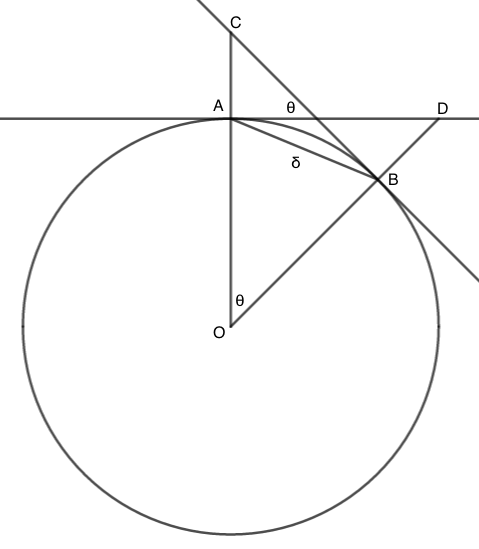
\includegraphics[width=\textwidth]{Circle-1.png}
                \caption{Drawing for Theorem 3.2.2}
              \end{subfigure}
              \begin{subfigure}[b]{0.32\textwidth}
                \centering
                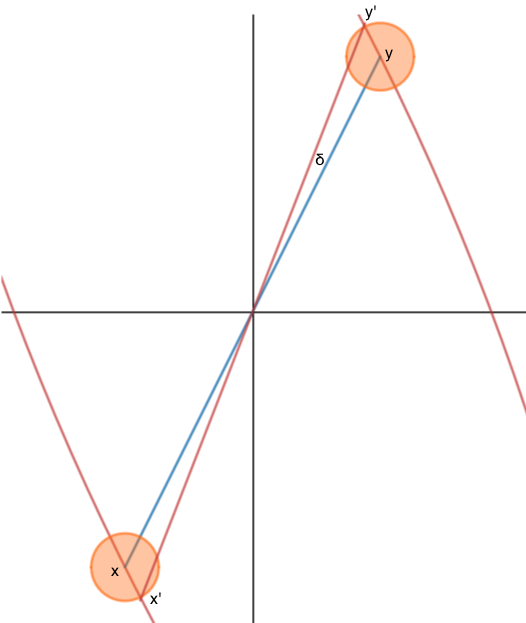
\includegraphics[width=\textwidth]{convex-1.png}
                \caption{Drawing for Theorem 3.2.3}
              \end{subfigure}
              \begin{subfigure}[b]{0.32\textwidth}
                \centering
                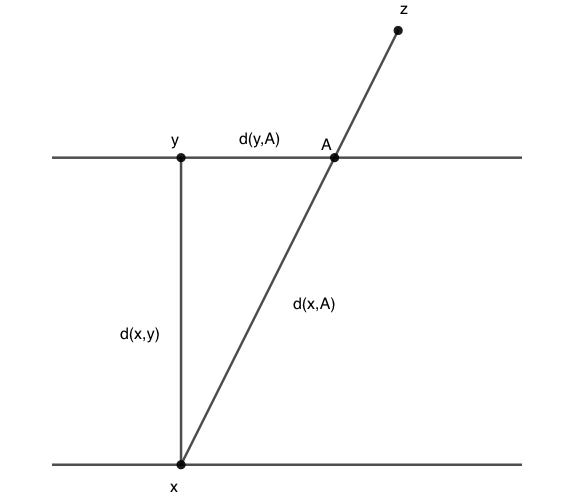
\includegraphics[width=\textwidth]{line-1.png}
                \caption{Drawing for Lemma 3.2.1}
              \end{subfigure}  
            \end{figure}
            \begin{theorem}
            If $K\subset \mathbb{R}^2$ is compact and convex, then $R_K(\theta)$ is continuous.
            \end{theorem}
            \begin{proof}
            For let $K$ be compact and convex, and without loss of generality suppose it contained within the unit disc and contains the origin. Let $\theta\in (0,2\pi)$ be given and let $\ell_{\theta}$ be a line through the origin making an angle $\theta$ with the horizontal. Let $x=(x_1,x_2),y=(y_1,y_2)\in K$ be such that $W_{\ell_{\theta}}(K) = d(x,y)$. Such points exist as $K$ is compact. Let $\varepsilon>0$ be given. About $x$, consider $B_{\frac{\varepsilon}{2}}(x)$, and similarly $B_{\frac{\varepsilon}{2}}(y)$. Neither of these are empty, as $K$ is convex. Let $x',y'\in K\cap(B_{\frac{\varepsilon}{2}}(x)\cup B_{\frac{\varepsilon}{2}}(y))$ be such that $d(x',y')$ is maximized. As this set is compact, such points exist. Let $\delta = \min\{|\theta-\frac{x_2'}{\sqrt{x_1'^2+x_2'^2}}|,|\theta-\frac{y_2'}{\sqrt{y_1'^2+y_2'^2}}|\}$. Then for $|\theta-\theta_0|<\delta$, $d(x,y)-\varepsilon \leq W_{\ell_{\theta_0}}(K)\leq d(x,y)+\varepsilon$, and thus $|W_{\ell_\theta}(K)-W_{\ell_{\theta_0}}(K)| < \varepsilon$.
            \end{proof}
            \begin{lemma}
            If $K$ is a compact subset of $\mathbb{R}^2$ and $x,y\in K$ such that $d(x,y)=D(K)$, then the lines perpendicular to $\overline{xy}$ at $x$ and $y$ contain all of $K$ in between.
            \end{lemma}
            \begin{proof}
            Suppose not. Let $\overline{X}$ be the line perpendicular to $\overline{xy}$ containing point $x$, and similarly define $\overline{Y}$. Suppose there is a point $z\in K$ that falls on the exterior of the region $\mathcal{U} = \{(x,y)\in \mathbb{R}^2: (x,y)\ \textrm{Lies Between } \overline{X}\ \textrm{and } \overline{Y}\}$. Note that $d(x,z)\ne d(y,z)$, as then $z$ would line between these two lines. Suppose $d(y,z)<d(x,z)$. Where the line $\overline{xz}$ cuts $\overline{Y}$ denote as $A$. But then $d(x,z) > d(x,A) = \sqrt{d(y,A)^2+d(x,y)^2}\geq d(x,y)$. A contradiction as $d(x,y) = D(K)$. Thus $z\in \mathcal{U}$.
            \end{proof}
            \begin{theorem}
            If $K\subset \mathbb{R}^2$ is compact and convex, then there are points $x,y\in K$ such that $\check{W}(K)=d(x,y)$.
            \end{theorem}
            \begin{proof}
            As $f_K(\theta)$ is continuous for convex compact set, and as it is continuous on a compact set $[0,2\pi]$, it attains its maximum. Let $\theta$ be such a maximum. Let $\ell_{\theta}$ be the line through the origin which makes an angle $\theta$ with the horizontal axis and consider set $K_{\ell_{\theta}}$. As $K$ is compact and $\ell_{\theta}$ is closed, $K_{\ell_{\theta}}$ is compact. Then $W=\{d(x,y):x,y\in K_{\ell_{\theta}}\}$ is bounded, has a least upper bound, and therefore there are points $x,y \in K$ such that $\check{W}(K)=d(x,y)$.
            \end{proof}
            \begin{theorem}
            If $K$ is a compact convex set of $\mathbb{R}^2$, then $D(K) = \check{W}(K)$.
            \end{theorem}
            \begin{proof}
            As $K$ is compact, $D(K)$ and $\check{W}(K)$ exists and there are points $x,y$ such that $d(x,y) = D(K)$ and points $x',y'$ such that $d(x',y') = \check{W}(K)$. Suppose $d(x',y')> d(x,y)$. A contradiction, as $d(x,y)$ is the diameter of $K$. So $d(x,y) \geq d(x',y')$. Now suppose $d(x,y)>d(x',y')$. But as $d(x',y')= \check{W}(K)$, $d(x',y')$ is the greatest length of any line segment that terminates in $K$ and such that perpendiculars at these terminating points contain all of $K$. But as $d(x,y)=D(K)$, the lines perpendicular to $\overline{xy}$ at $x$ and $y$ contain all of $K$, a contradiction. Thus $d(x',y') \geq d(x,y)$. But it was just showed that $d(x,y)\geq d(x',y')$. Thus, $d(x,y) = d(x',y')$. $D(K) = \check{W}(K)$.
            \end{proof}
            \begin{definition}
            If $Q$ is a convex polygon with interior (That is, positive area) in $\mathbb{R}^2$, then the perimeter of $Q$ is the sum of the lengths of its edges. 
            \end{definition}
            \begin{definition}
            The perimeter of a line segment $e$ is $P(e) = 2|e|$.
            \end{definition}
            \begin{remark}
            This is for the sake of continuity. If we take a rectangle of length $|e|$ and width $\frac{1}{n}$, then the perimeter is $2|e|+\frac{2}{n} \rightarrow 2|e|$ as $n\rightarrow \infty$. Thus, for the puprose of continuity we define the perimeter of line segments to be twice their length.
            \end{remark}
            \begin{theorem}[Cauchy's Perimeter Theorem]
            If $K$ is a compact convex subset of the plane, then $P(K) = \pi W(K)$.
            \end{theorem}
            \begin{proof}
            Suppose that $Q$ is a convex polygon with edges $e_1,\hdots, e_n$. At each $e_i$, let $\theta_i$ be the angle made with $e_i$ and the horizontal axis of $\mathbb{R}^2$. The mean width is $W(Q) = \frac{1}{2\pi}\int_{0}^{2\pi} W_{\ell_\theta}(Q)d\theta = \frac{1}{2\pi} \int_{0}^{2\pi} \frac{1}{2} \sum_{i=1}^{n} |e_i||\cos(\theta-\theta_i)|d\theta = \frac{1}{4\pi}\sum_{i=1}^{n} |e_i|\int_{0}^{2\pi} |\cos(\theta-\theta_i)|d\theta = \frac{1}{\pi} \sum_{i=1}^{n} |e_i| = \frac{1}{\pi} P(Q)$. Thus, $P(Q) = \pi W(Q)$. For any convex compact subset $K\subset \mathbb{R}^2$, we may find a polygon $Q$ that approximates the boundary with a perimeter $P(Q)$ that is as close to $P(K)$ and a width $W(Q)$ as close to $W(K)$ as desired. That is, for all $n\in \mathbb{N}$, we can obtain a polynomial $Q_n$ such that $\max\{|W(Q_n)-W(K)|,|P(K)-P(Q_n)|\}< \frac{1}{n}$. Then $|P(K)-\pi W(K)| = |P(K) - P(Q_n)+P(Q_n)-\pi W(Q_n)+\pi W(Q_n)-\pi W(K)| \leq |P(K)-P(Q_n)|+|P(Q_n)-\pi W(Q_n)|+\pi|W(Q_n)-W(K)| < \frac{1}{n} + 0 + \frac{\pi}{n} = \frac{1+\pi}{n} \rightarrow 0$. Thus, $P(K) = \pi W(K)$ for arbitrary convex compact subsets of the plane.
            \end{proof}
            \begin{theorem}
            There exist compact path-connected sets $K\subset \mathbb{R}^2$ such that $P(K) \ne \pi W(K)$.
            \end{theorem}
            \begin{proof}
            Consider the set $K = \{(x,y) \in \mathbb{R}^2: x^2+y^2=1, y\geq 0\}$. Then $P(K) = 2\pi$, but \\ $W(K) = \pi(\pi+2)$. To see this, consider the set $\mathcal{K} = \{(x,y)\in \mathbb{R}^2: x^2 + y^2 \leq 1, y\geq 0\}$. This is convex and has perimeter $\pi+2$ and therefore $W(\mathcal{K}) = \pi(\pi+2)$. But, as the image shows, $W(K) = W(\mathcal{K})$. That is, $W_{\ell_{\theta}}(K)$ is the length of the line segment $\overline{AB}$, as is $W_{\ell_{\theta}}(\mathcal{K})$. Therefore the averages $W(K)$ and $W(\mathcal{K})$ are the same. Thus, $P(K) \ne \pi W(K)$.
            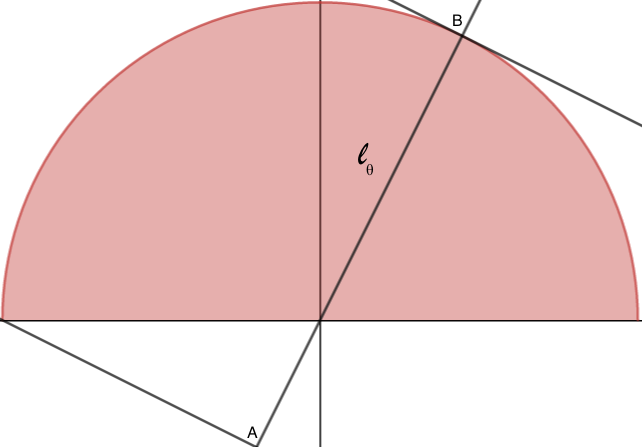
\includegraphics[scale=0.3]{semicircle-1.png}
            \end{proof}
            \begin{definition}
            A functional $f$ with respect to subset inclusion is said to be monotonic on a family of sets $\mathscr{P}$ if and only if $f(K)\leq f(L)$ for all $K,L \in \mathscr{P}$ such that $K\subset L$.
            \end{definition}
            \begin{theorem}
            If $K\subset L \in \mathscr{K}_2$, then $W_{\ell}(K) \leq W_{\ell}(L)$.
            \end{theorem}
            \begin{proof}
            For let $\pi_{\ell}:\mathbb{R}^2 \rightarrow \ell$ be the orthogonal projection map of $\mathbb{R}^2$ to $\ell$. Then $\pi_{\ell}(K)\leq \pi_{\ell}(L)$ as $K\subset L$, and thus $W_{\ell}(K)\leq W_{\ell}(L)$.
            \end{proof}
            \begin{theorem}
            If $K\subset L\in \mathscr{K}_2$, then $W(K)\leq W(L)$.
            \end{theorem}
            \begin{proof}
            For $W_{\ell}(K)\leq W_{\ell}(L)$, and thus $W(K)=\frac{1}{2\pi}\int_{0}^{2\pi}W_{\ell_{\theta}}(K)d\theta \leq \frac{1}{2\pi}\int_{0}^{2\pi}W_{\ell_{\theta}}(L)d\theta=W(L)$.
            \end{proof}
            \begin{theorem}
            If $K\subset L\in \mathscr{K}_2$, then $X_{\ell}(K)\leq X_{\ell}(L)$.
            \end{theorem}
            \begin{proof}
            For if $x\in \ell\cap K$, then $x\in \ell\cap L$, and thus $X_{\ell}(K)=\mu(\ell\cap K) \leq \mu(\ell\cap L)=X_{\ell}(L)$.
            \end{proof}
            \begin{theorem}
            If $K\subset L\subset \mathscr{K}_2$, then $D(K)\leq D(L)$.
            \end{theorem}
            \begin{proof}
            For suppose not. Suppose $D(K)>D(L)$. Then, there are points $x,y\in K$ such that $d(x,y)> \sup\{d(x',y'):x',y'\in L\}$. But as $K\subset L$, $x,y\in L$ and thus $d(x,y) \not> \sup\{d(x',y'):x',y'\in L\}$. Thus, $D(K)\leq D(L)$.
            \end{proof}
            \begin{theorem}
            If $K\subset L \subset \mathscr{K}_2$, then $R_K\leq R_L$.
            \end{theorem}
            \begin{proof}
            For suppose not. Suppose $R_K>R_L$. But as $K\subset L$, either this circle contains all of $L$ as well or it doesn't. But then $R_L \not<R_K$. Thus, $R_L\geq R_K$.
            \end{proof}
            \begin{theorem}
            If $K\subset L \in \mathscr{K}_2$, then $r_K \leq r_L$.
            \end{theorem}
            \begin{proof}
            For suppose not. Suppose $r_K> r_L$. But as the inscribed circle of radius $r_K$ fits entirely in $K$, and $K\subset L$, then it fits inside of $L$. But then $r_K \not > r_L$. Thus, $r_L \geq r_K$.
            \end{proof}
            \begin{theorem}
            If $K,L\in \mathscr{K}_2$ and $K\subset L$, then $P(K)\leq P(L)$.
            \end{theorem}
            \begin{proof}
            As $K\subset L\in  \mathscr{K}_2$, $W(K)\leq W(L)$. As $K$ and $L$ are convex, $P(K)=\pi W(K)$ and $P(L)=\pi W(L)$. Thus, $P(K) \leq \pi W(L) = P(L)$. Therefore, $P(K)\leq P(L)$.
            \end{proof}
            \begin{theorem}
            There exists sets $K,L\subset \mathbb{R}^2$ such that $L$ is convex, $K\subset L$, yet $P(K)>P(L)$.
            \end{theorem}
            \begin{proof}
            For let $L = \{(x,y)\in \mathbb{R}^2: x^2 + y^2 \leq 1\}$. Then $P(L) = 2\pi$. Let $K = \{(x,y)\in \mathbb{R}^2: -\sqrt{2}x\leq y \leq \sqrt{2}x,\frac{-1}{\sqrt{3}} \leq x \leq \frac{1}{\sqrt{3}} \lor \sqrt{2}x\leq y \leq -\sqrt{2}x,\frac{-1}{\sqrt{3}} \leq x \leq \frac{1}{\sqrt{3}} \}$. $P(K) = 4(1+ \sqrt{\frac{2}{3}}) \approx 7.26>2\pi$.
            \end{proof}
            \begin{figure}[H]
              \begin{subfigure}[b]{0.49\textwidth}
                 \centering
                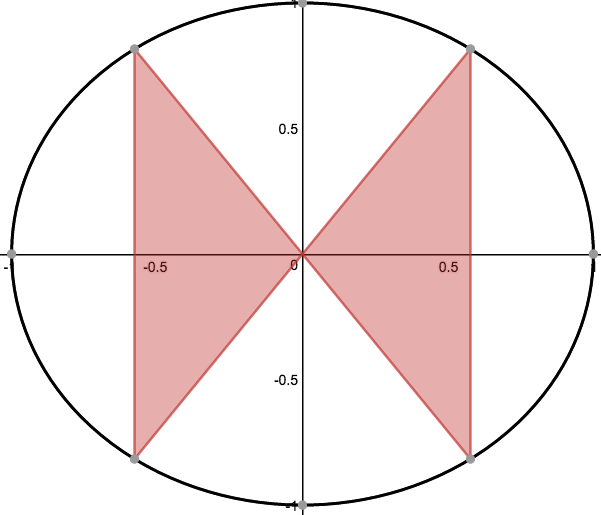
\includegraphics[width=\textwidth]{Circles-3.png}
                \caption{Drawing for Theorem 3.2.15}
              \end{subfigure}
              \begin{subfigure}[b]{0.49\textwidth}
                \centering
                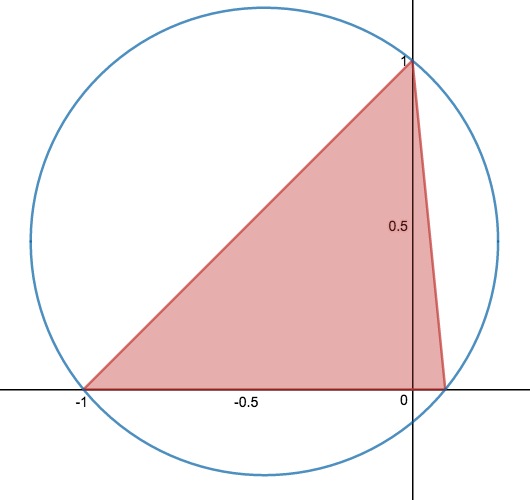
\includegraphics[width=\textwidth]{Circle-4.png}
                \caption{Drawing for Theorem 3.2.16}
              \end{subfigure}
            \end{figure}
            \begin{theorem}
            There exist compact convex sets in $\mathbb{R}^2$ such that $D(K) < 2R_K$.
            \end{theorem}
            \begin{proof}
            For consider the set $K=\{(x,y)\in \mathbb{R}^2: [0\leq y\leq x+1 \land x\geq 0]\lor [0\leq y\leq -10x+1\land x\geq 0]\}$. From Euclid, the smallest circle containing this triangle is the one defined by the three vertices (Three points define a triangle). This circle has the formula $(x+0.45)^2+(y-0.45)^2 = (0.45)^2 +(0.45+\frac{1}{10})^2$. Thus, $2R_K = \sqrt{0.45^2 +(0.45+\frac{1}{10})^2} > \sqrt{2} = D(K)$.
            \end{proof}
            \begin{theorem}
            If $K$ is a compact convex set in $\mathbb{R}^2$, then $D(K) \leq 2R_K$.
            \end{theorem}
            \begin{proof}
            For suppose not. Suppose $D(K) > 2R_K$. As $K$ is compact, there are points $x$ and $y$ in $K$ such that $d(x,y)=D(K)$. But then $d(x,y)>2R_K$, and thus at least one of $x$ or $y$ is not contained in the circle. A contradiction. Thus $D(K)\leq 2R_K$.
            \end{proof}
            \begin{theorem}
            If $K$ is a compact convex set in $\mathbb{R}^2$, then $2\pi r_K \leq P(K)$.
            \end{theorem}
            \begin{proof}
            From Calculus of Variations we know that the circle maximizes the area contained with a set of perimeter $p$. As the inscribed circle has perimeter $2\pi r_K$ and as the circle is a subset of $K$, it is true that $A(K)$ is greater than or equal the area of the circle. Thus, $P(K)\geq 2\pi r_K$.
            \end{proof}
            \begin{theorem}
            For a compact convex set of $\mathbb{R}^2$, $P(K) \leq 2\pi R_K$.
            \end{theorem}
            \begin{proof}
            As $K$ is convex, $P(K) = \pi W(K) \leq \pi \check{W}(K) = \pi D(K) \leq 2\pi R_K$.
            \end{proof}
            \begin{theorem}
            If $K$ is a compact and convex subset of $\mathbb{R}^2$, then $2D(K)\leq P(K)$.
            \end{theorem}
            \begin{proof}
            Suppose not. Suppose $2D(K) >P(K)$. As $K$ is compact and convex, there exist points $x,y\in K$ such that $d(x,y) = D(K)$. But as $K$ is convex, the line contained between $x,y$ in contained in $K$. Thus, $P(\overline{xy}) = 2D(K)$. But as $\overline{xy}\subset K$, $P(K)>P(\overline{xy})$, a contradiction. Thus, $2D(K) \leq P(K)$.
            \end{proof}
            \begin{theorem}
            There exist compact convex subsets of $\mathbb{R}^2$ such that $2D(K) = P(K)$.
            \end{theorem}
            \begin{proof}
            For take a straight line segment of length $\ell$. Then $D(K) = \ell$, $P(K) = 2\ell$, and thus $2D(K) = P(K)$.
            \end{proof}
            \begin{theorem}
            If $K$ is a compact convex subset of $\mathbb{R}^2$, then $P(K) \leq \pi D(K)$.
            \end{theorem}
            \begin{proof}
            From Cauchy's Perimeter theorem, $P(K) = \pi W(K) \leq \pi \check{W}(K) = \pi D(K)$.
            \end{proof}
            \begin{theorem}
            For a compact convex subset $K$ of $\mathbb{R}^2$, $P(K) = \pi D(K)$ if and only if $W_{\ell}(K)$ is a constant.
            \end{theorem}
            \begin{proof}
            For then $\frac{1}{2\pi} \int_{0}^{2\pi} W_{\ell_{\theta}}(K) d\theta = \check{W}(K)$. But as $W_{\ell_{\theta}}(K)$ is continuous for compact convex bodies, it must be true that $W_{\ell_{\theta}}(K) = \check{W}(K)$ for all $\ell_{\theta}$. Thus, $K$ is of constant width.
            \end{proof}
            \begin{remark}
            There are many types of shapes that have constant width besides discs. The Reuleaux Triangle is such an example.
            \end{remark}
            Triangles are the simplest convex bodies in the plane other than points and lines. Any convex polygon can be written as the union of triangles with disjoint interiors. 
            \begin{theorem}
            If $\Delta_s$ is an equilateral triangle with edge length $s$, then $\Delta_s$ has the following properties:
            \begin{enumerate}
            \begin{multicols}{5}
            \item $A(\Delta_s) = \frac{\sqrt{3}}{4}s^2$
            \item $P(\Delta_s) = 3s$
            \item $W(\Delta_s) = \frac{3s}{\pi}$
            \item $R_{\Delta_s} = \frac{1}{\sqrt{3}}s$
            \item $r_{\Delta_s} = \frac{1}{2\sqrt{3}}s$
            \end{multicols}
            \end{enumerate}
            \end{theorem}
            \begin{proof}
            In order:
            \begin{enumerate}
                \item From Pythagoras, $A(\Delta_s) =2\times\big[\frac{1}{2}(\frac{1}{2}s)(\frac{\sqrt{3}}{2}s)\big] = \frac{\sqrt{3}}{4}s^2$
                \item There are three edges, each of length $s$, and thus $P(\Delta_s) = 3s$.
                \item $W(\Delta_s) = \frac{1}{\pi}P(\Delta_s) = \frac{3s}{\pi}$
                \item The circumcircle gives the following equations:
                \begin{enumerate}
                    \item $R_{\Delta_s}^2=\frac{s^2}{4}+h^2$
                    \item $h+R_{\Delta_s} = \frac{\sqrt{3}}{2}s$
                \end{enumerate}
                This has solution $R_{\Delta_s}=\frac{1}{\sqrt{3}}s$
                \item $r_{\Delta_s} = \frac{R_{\Delta_s}}{2}= \frac{1}{2\sqrt{3}}s$
            \end{enumerate}
            \end{proof}
            \begin{theorem}
            If $T$ is a triangle in the plane, then there is a linear transformation $\psi$ such that $\psi T$ is equilateral.
            \end{theorem}
            \begin{proof}
            For let $T$ be a triangle with vertices $a=(x_1,y_1)$, $b=(x_2,y_2)$, $c=(x_3,y_3)$. Let $A = d(b,c)$, $B=d(a,c)$, and $C=d(a,b)$. Suppose If $A=B=C$, we are done. Thus, suppose $C\geq B >A$. At point $a$ and with radius $C$, construct the circle $b,c',d$, and point $b$ and with radius $C$, construct the circle $a,c',e$. If we can shift $c$ to $c'$ in a linear fashion, we are done. Let $\psi =$
            \end{proof}
            \begin{theorem}
            If $T$ is a triangle with edges $a,b,c$ and opposite angles $\alpha,\beta,\gamma$, respectively, then $A(T) = \frac{\sin(\alpha)}{2}bc = \frac{\sin(\beta)}{2}ac = \frac{\sin(\gamma)}{2}ab$
            \end{theorem}
            \begin{proof}
            Suppose the triangle is acute. The proof is symmetric for all sides, so we prove it for just $\alpha$. Note that the perpendicular $h$ dropped from the vertex of $a$ onto $b$ satisfies $h^2+\ell_1^2 = c^2$ and $h^2+\ell_2^2 = a^2$, where $\ell_1+\ell_2 = b$. Then $\sin(\alpha) = \frac{h}{c}$ and $A(T) = \frac{1}{2}h\ell_1 + \frac{h}{2}h\ell_2 = \frac{h}{2}(\ell_1+\ell_2)h = \frac{1}{2}bh = \frac{1}{2}bc\sin(\alpha)$. An identical argument works for obtuse triangles.
            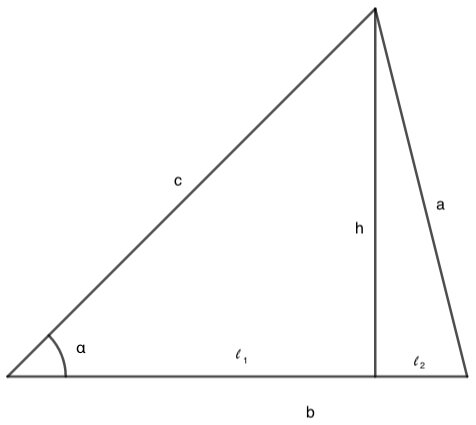
\includegraphics[scale=0.3]{triangle-1.png}
            \end{proof}
            \begin{corollary}[The Law of Sines]
            For a triangle with edges $a,b,c$ and opposite angles $\alpha,\beta,\gamma$, $\frac{\sin(\alpha)}{a} = \frac{\sin(\beta)}{b} = \frac{\sin(\gamma)}{c}$
            \end{corollary}
            \begin{proof}
            From the previous theorem, divide by $\frac{abc}{2}$ to obtain the result.
            \end{proof}
            \begin{theorem}[The Law of Cosines]
            Given a triangle with lengths $a,b,c$ and opposite edges $\alpha,\beta,\gamma$, $c^2=a^2+b^2-2ab\cos(\gamma)$.
            \end{theorem}
            \begin{proof}
            If $\gamma=\frac{\pi}{2}$, this is Pythagoras' Theorem. Thus, suppose $0<\gamma < \frac{\pi}{2}$. Where $c$ and $a$ meet, drop a perpendicular onto $c$ and call this $h$. $h$ satisfies $h^2+\ell_1^2 = c^2$ and $h^2+\ell_2^2=a^2$ from Pythagoras' Theorem, where $\ell_1+\ell_2 = b$. But $\ell_2 = a\cos(\gamma)$, so $\ell_1 = b-a\cos(\gamma)$. Thus $c^2 = h^2 + b^2 +a^2\cos^2(\gamma)-2ab\cos(\gamma)$. But $h = a\sin(\gamma)$. Thus, $c^2 = b^2 + a^2 \cos^2(\gamma)+\sin^2(\gamma)-2ab\cos(\gamma) = b^2 + a^2(\sin^2(\gamma)+\cos^2(\gamma))-2ab\cos(\gamma) = a^2 + b^2 -2ab\cos(\gamma)$. A similar construction is done if $\frac{\pi}{2}<\gamma < \pi$.
            \end{proof}
            \begin{theorem}
            Given a triangle $\Delta$ with lengths $a\leq b\leq c$, $D(\Delta)=c$.
            \end{theorem}
            \begin{proof}
            At the midpoint of $c$, and with radius $c$, construct a circle. This circle contains the entirety of $\Delta$, and thus for all points $x,y\in \Delta$, $d(x,y)\leq c$. Thus, $c=D(\Delta)$.
            \end{proof}
            \begin{theorem}[Heron's Formula]
            For a triangle with lengths $a,b,c>0$, $A(T)^2 = \frac{1}{16}(a+b+c)(-a+b+c)(a-b+c)(a+b-c)$.
            \end{theorem}
            \begin{proof}
            For $A(T) = \frac{1}{2}ab \sin(\gamma) = \frac{1}{2}ab\sqrt{1-\cos^2(\gamma)} = \frac{1}{4}\sqrt{4a^2 b^2 - (a+b-c)^2}=\\ \frac{1}{4}\sqrt{(2ab-(a^2+b^2-c^2))(2ab+(a^2+b^2+c^2))} = \frac{1}{4}\sqrt{(c^2-(a-b)^2)((a+b)^2-c^2)} = \\ \frac{1}{4}\sqrt{(a+b+c)(-a+b+c)(a-b+c)(a+b-c)}$. Squaring this gives the result.
            \end{proof}
            \begin{theorem}
            For any triangle $\Delta$, $r_{\Delta}P(\Delta) = 2A(\Delta)$.
            \end{theorem}
            \begin{proof}
            For let $\Delta$ has sides $a,b,c$, with opposite angles $\alpha, \beta, \gamma$, respectively. Then $A(\Delta) = \frac{ab}{2}\sin(\gamma)$ and $P(\Delta)=a+b+c$. Thus, $\frac{2A(\Delta)}{P(\Delta)} = \frac{ab\sin(\gamma)}{a+b+c}$. But this is the radius of the incircle of $\Delta$. Therefore, etc.
            \end{proof}
            \begin{theorem}[Viviani's Theorem: Page 17]
            \end{theorem}
            \begin{theorem}
            There exist convex polygon's such that the inradius is not unique.
            \end{theorem}
            \begin{proof}
            For consider the rectangle $[0,2]\times [0,1]$. The diameter of any circle that sits inside this body must be at most $1$, and thus the radius is at most $\frac{1}{2}$. However, there are multiple circles that achieve this. For example $(x-\frac{1}{2})^2+(y-\frac{1}{2})^2=\frac{1}{2}$ and $(x-\frac{3}{2})^2+(y-\frac{3}{2})^2=\frac{1}{2}$.
            \end{proof}
            \begin{theorem}
            For an acute triangle, $\frac{2(A)}{abc} = \frac{1}{R_T}$.
            \end{theorem}
            \begin{theorem}
            If $\Delta$ is a triangle with vertices $A,B,C$ and sides $a,b,c$, then given a circle that contains $A,B,C$, the radius of this circle $R$ satisfies $\frac{1}{R} =\frac{2A(\Delta)}{abc}$
            \end{theorem}
            \begin{definition}
            If $K\in \mathscr{K}_2$, then $-K = \{-x:x\in K\}$.
            \end{definition}
            \begin{theorem}
            If $K\in \mathscr{K}_2$, then $W_{\ell}(K) = W_{\ell}(-K)$.
            \end{theorem}
            \begin{proof}
            For let $x,y\in K$ be such that $d(x,y) = W_{\ell}(K)$. Then $d(-x,-y) = W_{\ell}(-K) = d(x,y)$. Therefore, etc.
            \end{proof}
            \begin{theorem}
            There exist sets $K$ and $L$ such that $W_{\ell}(K)<W_{\ell}(L)$ for all $\ell$ yet $K\not\subset L$ for any translation or rotation of $K$.
            \end{theorem}
            \begin{definition}
            For $K\in \mathscr{K}$ and unit vector $u$, $\bar{X}_{u}(K)$ is the mean value of $X_{\ell}(K)$ over all lines $\ell$ parallel to $u$ such that $X_{\ell}(K)>0$.
            \end{definition}
            \begin{theorem}
            For $K\in \mathscr{K}_2$, $\bar{X}_{u}(K) = W_{\ell}(K)=A(K)$.
            \end{theorem}
        \section{On Uniform Convergence}
            \begin{definition}
                A sequence of functions $f_n$ is said to converge
                point-wise on a set $A$ to a function $f$, if
                $\forall\varepsilon>0$ and $\forall x\in A$, there is
                an $N\in\mathbb{N}$ such that $n>N \Rightarrow
                |f(x)-f_n(x)|<\varepsilon$.
            \end{definition}
            \begin{definition}
                A sequence of functions $f_n$ converge uniformly on a
                set $A$ to $f$ if and only if $\forall \varepsilon>0$
                $\exists N\in\mathbb{N}$ such that $\forall x \in A$
                and $n>N$, $|f(x) -f_n(x)|<\varepsilon$.
            \end{definition}
            \begin{definition}
                A sequence of functions $f_n$ are point-wise
                equicontinuous on a set $A$ if and only if
                $\forall_{\varepsilon>0}\forall_{x\in A}
                \exists_{\delta>0}\forall_{n\in\mathbb{N}}:
                |x-x_0|<\delta\Rightarrow|f_{n}(x)-f_{n}(x_0)|<
                \varepsilon$
            \end{definition}
            \begin{definition}
                A sequence of functions $f_n$ are uniformly
                equicontinuous on a set A if and only if
                $\forall_{\varepsilon>0}\exists_{\delta>0}
                \forall_{x\in A}\forall_{n\in\mathbb{N}}:
                |x-x_{0}|<\delta\Rightarrow|f_{n}(x)-f_{n}(x_{0})|<
                \varepsilon$.
            \end{definition}
            \begin{definition}
                A subset $A$ of the real line is open if
                $\forall_{x\in A}\exists_{r>0}:
                \forall_{y\in (x-r,x+r)},y\in A$.
            \end{definition}
            \begin{definition}
                An open cover $\Delta$ of a set $A\subset S$ is a set
                of open subsets $A_k\subset S$, such that
                $A\subset\cup_{k\in I}A_{k}$, where $I$ is some
                index, countable or uncountable.
            \end{definition}
            \begin{definition}
                A set $A$ is said to be compact if and
                only if for all open coverings $\Delta$ there is
                a finite sub-cover $\Delta_0\subset \Delta$, such
                that $A\subset \cup_{A_k \in \Delta_0} A_k$.
            \end{definition}
            \begin{theorem}
                [Heine-Borel Theorem]
                Any closed-bounded subset of the real line is compact. 
            \end{theorem}
            \begin{proof}
                For let $A$ be a closed and bounded subset of
                $\mathbb{R}$ with least upper bound $b$ and
                greatest lower bound $a$. Let $\Delta$ be an
                open covering, and let $X$ be the set of
                points $y\in A$ such that for all $s<y$ such
                that $s\in A$, there is a finite refinement
                of $\Delta$ which covers these points. $X$ is
                non-empty, as $a\in X$. The set $X$ is bounded,
                as for all points $y\in X$ we have that
                $a\leq y\leq b$. As bounded sets have a least
                upper bound, let $x$ be the least upper bound.
                Suppose $x<b$. As $x\in [a,b]$, there exists an
                element $A_k$ of $\Delta$ such that $x \in A_k$.
                But as $A_k$ is open and therefore there is an
                $r>0$ such that
                $y\in (x-r,x+r)\Rightarrow y \in A_k$.
                But then $y=x+\frac{r}{2}>x$ and
                $y\in A_k$. Therefore x is not the
                least upper bound as we have found an
                element in $X$ greater than $x$.
                Therefore $x\not<b$. And thus $x=b$.
            \end{proof}
            \begin{theorem}
                If a sequence of functions are
                point-wise equicontinuous on a closed
                and bounded set, then they are
                uniformly equicontinuous.
            \end{theorem}
            \begin{proof}
                For let $A$ be a closed bounded subset
                of $\mathbb{R}$, and let $f_n(x)$ be a sequence
                of point-wise equicontinuous functions on $A$.
                As the set is closed and bounded, it is compact
                by the Heine-Borel theorem. Let $\varepsilon>0$
                be given. For $x\in A$, define the function
                $\delta(x)%
                 =\min\{\sup\{\delta>0:|x-x_0|<\delta,\ x_0\in A%
                  \Rightarrow |f_n(x)-f_n(x_0)|<\frac{\varepsilon}{2}$,
                $\forall n\in\mathbb{N}\},b-a\}$.
                Construct the open covering $\mathcal{U}$ as
                follows:
                $\mathcal{U}=\{(x-\delta(x),x+\delta(x)):\ x\in A\}$.
                This is an open covering, as every set in
                $\mathcal{U}$ is open, and for all
                $x\in A$, $x\in(x-\delta(x),x+\delta(x))\in\mathcal{U}$.
                But as $A$ is compact, there is a finite sub-cover.
                Let $a=x_0<x_1<...<x_{n-1}<x_n=b$ be the centers
                of the remaining open sets in the sub-cover.
                Further refine this sub-covering as follows: If
                $(x_j-\delta(x_j),x_j+\delta(x_j))%
                 \subset (x_k-\delta(x_k),x_k+\delta(x_k))$
                for $j\ne k$, then remove it from the sub-cover as
                it is superfluous. We now have a set of points
                $a=z_0<z_1<...<z_{N-1}<z_N=b$ such that
                $A\subset\cup_{i=0}^{N} (z_i-\delta(z_i),z_i+\delta(z_i))$.
                Let
                $\delta%
                 =\min\{\delta(z_0),...,\delta(z_N),\delta(b),%
                        \frac{(a+\delta(a))-(z_1-\delta(z_1))}{2},%
                        ...,%
                        \frac{(z_{N-1}+\delta(z_{N-1}))-(b-\delta(b))}{2}\}$.
                That is, $\delta$ is the smallest of the $\delta(z_i)$,
                or half of the smallest intersection of two consecutive
                intervals. Let $x\in A$ be arbitrary. If $(x-\delta,x+\delta)$
                is contained entirely in one of the
                $(z_i-\delta(z_i),z_i+\delta(z_i))$ sets, then we have
                that $|x-x_0|<\delta \Rightarrow |x-x_0| <\delta(z_i) \Rightarrow |f_n(x)-f_n(x_0)|<\frac{\varepsilon}{2}$ for all $n\in\mathbb{N}$.
                Suppose that $(x-\delta,x+\delta)$ is contained in two of
                the $(x-\delta(z_i),x+\delta(z_i))$ sets. Note, it cannot
                be in three or more as we have refined the sub-cover in
                such a manner as to prevent this. Let $y$ be the center
                of the intersection of these two sets. Then we have that
                for $|x-x_0|<\delta$, then
                $|f_n(x)-f_n(x_0)|%
                 =|f_n(x)-f_n(y)+f_n(y)-f_n(x_0)|%
                 \leq|f_n(x)-f_n(y)|+|f_n(y)-f_n(x_0)|$.
                But $|x-y|$ and $|x_0-y|$ are less than
                $\frac{(z_i + \delta(z_i))-(z_{i+1}-\delta(z_{i+1}))}{2}$
                apart, and therefore $|f_n(x)-f_n(y)|<\frac{\varepsilon}{2}$,
                and $|f_n(y)-f_n(x_0)|<\frac{\varepsilon}{2}$.
                Therefore, $|f_n(x)-f_n(x_0)|<\varepsilon$.
                And as $x$ is arbitrary,
                $f_n(x)$ is uniformly equicontinuous.
            \end{proof}
            \begin{theorem}
                If a sequence of point-wise equicontinuous functions converge, then the limit is point-wise continuous.
            \end{theorem}
            \begin{proof}
                For let $f_n:A\rightarrow \mathbb{R}$ be equicontinuous, $\varepsilon>0$ and $x\in A$ be given. Choose $\delta>0$ to satisfy the criterion of equicontinuity at $x$. Let $x_0$ be an arbitrary point in $(x-\delta,x+\delta)\cap A$. It suffices to show that $|f(x) - f(x_0)|<\varepsilon$. As $f_n \rightarrow f$ we have that $\exists N_1 \in\mathbb{N}$ such that $n>N_1\Rightarrow |f(x) - f_n(x)|<\varepsilon$. We also have that $\exists N_2 \in \mathbb{N}$ such that $n>N_2 \Rightarrow |f(x_0)-f_n(x_0)|<\varepsilon$. Let $N=\max\{N_1,N_2\}+1$. But we have that $|f(x) - f(x_0)| = |f(x) - f_N(x) + f_N(x)-f_N(x_0) + f_N(x_0) - f(x_0)|\leq |f(x) - f_n(x)| + |f_n(x)-f_n(x_0)| + |f_n(x_0) - f(x_0)| < 3\varepsilon$. $f$ is continuous.
            \end{proof}
            \begin{theorem}
                If $f_n \rightarrow f$ on a closed bounded subset of $\mathbb{R}$, and if $f_n$ is equicontinuous, then the convergence is uniform.
            \end{theorem}
            \begin{proof}
                Let $A$ be a closed bounded subset of $\mathbb{R}$, $f_n(x)$ a sequence of equicontinuous functions, and let $\varepsilon>0$ be given. As $f_n(x)$ is equicontinuous on a closed bounded set, it is uniformly equicontinuous. But the limit of equicontinuous functions is continuous. Let $\delta>0$ be such that, $\forall x\in A$, $\forall n\in\mathbb{N}$, $|x-x_0|<\delta, x_0\in A \Rightarrow |f_n(x)-f_n(x_0)|<\frac{\varepsilon}{3}$ and $|x-x_0|<\delta \Rightarrow |f(x)-f(x_0)|<\frac{\varepsilon}{3}$. Let $\mathcal{U} = \{(x-\frac{\delta}{2},x+\frac{\delta}{2}): x\in A\}$. This is an open cover of $A$ and thus there is a finite subcover. Let $x_0<x_1<\hdots<x_n$ be the centers of the finitely many sets $(x_k-\frac{\delta}{2},x_k+\frac{\delta}{2})$ that cover $A$. There is thus another finite sequence of positive integers, $N_0, N_1,... N_n$, such that $n>N_k \Rightarrow |f(x_k)-f_n(x_k)|<\frac{\varepsilon}{3}$, for $k=0,1,2,...,n$. Let $N= \max\{N_0, N_1, ..., N_n\}$.It suffices to show that, for any point $x_0 \in A$, for all $n>N$, $|f(x_0)-f_n(x_0)|<\varepsilon$. Let $x_0$ be arbitrary and let $x_k$ be the nearest point to $x_0$ in the above sequence (If there are two nearest points, pick your favorite). Then we have that, for $n>N$, $|f(x_0) - f_n(x_0)| = |f(x_0)-f(x_k)+f(x_k)-f_n(x_k)+f_n(x_k)-f_n(x_0)|\leq |f(x_k)-f(x_0)|+|f(x_k)-f_n(x_k)|+|f_n(x_k)-f_n(x_0)|<\varepsilon$. The convergence is uniform.
            \end{proof}
            \begin{theorem}
                [Integration of a Uniformly Convergent Sequence of Functions]
                If $f_n\rightarrow f$ uniformly on a closed bounded set $A$ with $g.u.b(A)=a$, then $\int_{a}^{x} f_n \rightarrow \int_{a}^{x} f$ uniformly on $A$.
            \end{theorem}
            \begin{proof}
                Let $\varepsilon >0$ be given, let $b=l.u.b.(A)$, and choose $N\in\mathbb{N}$ such that $n>N\Rightarrow |f(x)-f_n(x)|<\frac{\varepsilon}{b-a}$. Then we have $|\int_{a}^{x} f_n - \int_{a}^{x} f| = |\int_{a}^{x} (f_n-f)| \leq \int_{a}^{x} |f_n-f| < \int_{a}^{x} \frac{\varepsilon}{b-a}= \frac{\varepsilon}{b-a}(x-a) \leq \varepsilon$.
            \end{proof}
            \begin{theorem}
                [Differentiation of a Uniformly Convergent Sequence of Functions]
                If $f_n'\rightarrow g$ uniformly on a closed bounded set $A$, and if $f_n \rightarrow f$ on $A$, then $f'=g$.
            \end{theorem}
            \begin{proof}
                Let $a=g.u.b.(A)$ and $b=l.u.b.(A)$. We have that $f_n(x) - f_n(a) = \int_{a}^{x}f_n' \rightarrow \int_{a}^{x}g$ uniformly. But $f_n(x)-f_n(a) \rightarrow f(x) - f(a)$. Therefore $f'(x)=\frac{d}{dx}(f(x)-f(a)) = \frac{d}{dx}\int_{a}^{x} g = g(x)$. $f' = g$.
            \end{proof}
            \begin{theorem}
                [The Product of a Uniformly Convergence Sequence and a Bounded Function]
                If $f_n \rightarrow f$ uniformly, and if $g$ is a bounded function, then $f_n g \rightarrow fg$ uniformly.
            \end{theorem}
            \begin{proof}
                For let $\varepsilon>0$ and $x$ be given, and let $g$ be a bounded function with bound $M$, and choose $N\in\mathbb{N}$ such that $n>N \Rightarrow |f(x)-f_n(x)|<\frac{\varepsilon}{M}$. Then we have that $|f(x)g(x)-f_n(x)g(x)| = |g(x)||f(x)-f_n(x)| < M|f(x)-f_n(x)| <\varepsilon$.
            \end{proof}
            \begin{theorem}
                If $f$ is continuous on a compact set $A$, then it is uniformly continuous.
            \end{theorem}
            \begin{proof}
                For let $\varepsilon>0$ be given, let $a=g.u.b.(A)$, $b=l.u.b.(A)$, and for $x\in A$ define $\delta(x) = \min\{\sup\{\delta>0: |x-x_0|<\delta,x_0\in A\Rightarrow |f(x)-f(x_0)|<\frac{\varepsilon}{2}\},b-a\}$. Let $\Delta = \{(x-\delta(x),x+\delta(x)):x\in A\}$. Then $\Delta$ is an open cover of $A$ and therefore there is an open subscover. Let $x_k$ be the centers of the finitely many sets $(x_k-\delta(x_k),x+\delta(x_k))$ that cover $A$. Further refine this by removing overlaps. That is, if $(x_i-\delta(x_i),x_i+\delta(x_i))\subset (x_j-\delta(x_j),x_j+\delta(x_k))$ for $i\ne j$, then remove it for it is superfluous. We thus obtain a new sequence $z_1,\hdots, z_N$ such that the intervals $(z_k-\delta(z_k),z_k+\delta(z_k))$ cover $A$. Define $\delta = \min\{\delta(z_1),\hdots,\delta(z_N), \frac{(z_0+\delta(z_0))-(z_1-\delta(z_1))}{2},\hdots,(\frac{z_{N-1}+\delta(z_{N-1}))-(z_{N}-\delta(z_{N})}{2}\}$. Let $x,x_0\in A$ such that $|x-x_0|<\delta$. Let $x_k$ be the closest point in the sequence to $x$ (If there are two such points, pick your favorite). Then $|f(x)-f(x_0)|=|f(x)-f(x_k)+f(x_k)-f(x_0)|\leq |f(x)-f(x_k)|+|f(x_k)-f(x_0)|<\varepsilon$
            \end{proof}
            \begin{remark}
                The proof of this is a mimicry of the proof that equicontinuity on a compact set implies uniform equicontinuity.
            \end{remark}
            \begin{definition}
                A set $A$ is called sequentially compact if given a sequence $x_n\in A$, there is a convergent subsequence $x_{n_k}$.
            \end{definition}
            \begin{theorem}
                Compact sets of $\mathbb{R}$ are sequentially compact.
            \end{theorem}
            \begin{proof}
                Let $A$ be a compact set in $\mathbb{R}$, and let $x_n$ be a sequence in $A$. A point $x\in A$ is the limit of a subsequence of $x_n$ if for every $\varepsilon>0$ there are infinitely many of the $x_n$ such that $|x-x_n|<\varepsilon$. Suppose there is no such point. That is, for each $x\in A$ only finitely many of the $x_n$ lie within sufficiently small $\varepsilon-$neighborhoods. Let $\varepsilon(x) = \sup\{\varepsilon>0:\textrm{Only finitely many }x_n \textrm{ lie within } \varepsilon \textrm{ of } x\}$. Define $E=\{(x-\varepsilon(x)<x+\varepsilon(x)):x\in A\}$. This is an open cover of $A$, and therefore there is a finite subcover. Thus, at least one of the finitely many intervals $(x-\varepsilon(x),x+\varepsilon(x))$ must contain infinitely many of the $x_n$, a contradiction. Thus there is a convergent subsequence.
            \end{proof}
            \begin{theorem}
                Continuous functions on compact sets are bounded.
            \end{theorem}
            \begin{proof}
                For suppose not. Let $f:A\rightarrow \mathbb{R}$ be a continuous function on a compact set $A$, and let $x_n$ be a sequence of points in $A$ such that $f(x_n)>n$. Such a sequence must exist as $f$ is not bounded. As $A$ is compact, there must a point $x\in A$ such that some subsequence $x_{n_k}$ that converges to $x$. Let $\varepsilon >0$. Then, as $f$ is continuous, there is a $\delta>0$ such that $|x-x_0|<\delta,\ x_0\in A\Rightarrow |f(x)-f(x_0)|<\varepsilon$. But then for all points $x_{n_k}$ such that $|x-x_{n_k}|<\delta$, $-\varepsilon<f(x_{n_k})-f(x)<\varepsilon \Rightarrow f(x)-\varepsilon < f(x_{n_k})<f(x)+\varepsilon$. A contradiction as $f(x_{n_k})$ is unbounded. Thus, $f$ is bounded.
            \end{proof}
            \begin{corollary}
                Continuous functions on compact sets attain their maximum and minimum.
            \end{corollary}
            \begin{proof}
                For let $f:A\rightarrow \mathbb{R}$ be a continuous function on a compact set $A$. Let $f(A) = \{y\in \mathbb{R}:\exists x\in A|\ f(x)=y\}$. (This is called the image of $A$ under $f$). As $f$ is continuous, it is bounded, and thus the set $f(A)$ is bounded. But bounded sets have an l.u.b. and a g.u.b. Therefore, etc.
            \end{proof}
            \begin{lemma}
                [Uniform Limit Theorem]
                If $f_n\rightarrow f$ uniformly, and if the $f_n$ are continuous, then $f$ is continuous.
            \end{lemma}
            \begin{proof}
                For let $\varepsilon>0$ be given and let $x\in A$. Let $N\in \mathbb{N}$ such that $n>N$ implies $|f(\chi)-f_n(\chi)|<\frac{\varepsilon}{3}$ for all $\chi\in A$. Let $\delta>0$ be chosen such that $|x-x_0|<\delta, x_0\in A\Rightarrow |f_N(x)-f_N(x_0)|<\frac{\varepsilon}{3}$. Then  $|f(x)-f(x_0)|=|f(x)-f_N(x)+f_N(x)-f_N(x_0)+f_N(x_0)-f(x_0)|\leq |f(x)-f_N(x_0)|+|f_N(x)-f_N(x_0)|+|f(x_0)-f_N(x_0)|<\varepsilon$.
            \end{proof}
            \begin{theorem}
                If $f_ng\rightarrow fg$ uniformly on a compact set $A$, and if $g$ is continuous and positive, then $f_n\rightarrow f$ uniformly.
            \end{theorem}
            \begin{proof}
                As $g$ is positive on a compact set, its minimum is also positive and is attained on $A$. Let $x_{min}\in A$ be such a minimum of $g$. Let $\varepsilon>0$ be given and let $N\in \mathbb{N}$ be such that for $n>N$, $|f_ng-fg|<\varepsilon\cdot g(x_{min})$. Then, $|f_ng-fg|=|g||f_n-f|\leq |g(x_{min})||f_n-f|<\varepsilon \cdot g(x_{min})\Rightarrow |f_n-f|<\varepsilon$.
            \end{proof}
            \begin{lemma}
                If $f_n'$ is uniformly bounded, then $f_n$ is equicontinuous.
            \end{lemma}
            \begin{proof}
                For let $M$ be such a bound for $f_n'$ and let $\varepsilon>0$ be given. Choose $\delta = \frac{\varepsilon}{M}$. Then for $x,x_0\in A$ and $|x-x_0|<\delta$, $|\int_{x_0}^{x}f_n'| =|f_n(x)-f_n(x_0)| \leq \int_{x_0}^{x}|f_n'| \leq (x-x_0)M < \varepsilon$.
            \end{proof}
            \begin{theorem}
                If $f_n'$ is uniformly bounded, and if $f_n \rightarrow f$ on a closed and bounded subset of $\mathbb{R}$, then the convergence is uniform.
            \end{theorem}
            \begin{proof}
                From the previous lemma, $f_n$ is equicontinuous. But a sequence of equicontinuous functions on a compact set is uniformly equicontinuous. And a sequence of uniformly equicontinuous functions that converge does so uniformly. Therefore, etc.
            \end{proof}
            \begin{theorem}
                If $f_n \rightarrow f$, $f_n'\rightarrow g$ and if $f_n''-f_n'$ is uniformly bounded on a closed bounded set, then the convergences are uniform and $f' = g$.
            \end{theorem}
            \begin{proof}
                Let $A$ be the closed bounded set under consideration. First note that as $f''_n - f'_n$ is uniformly bounded, $f_n'-f_n$ is equicontinuous. But as $f_n'$ and $f_n$ converge to $g$ and $f$, respectively, then $f_n'-f_n$ converges to $g-f$ uniformly. Let $M$ be a bounded for $f_n''-f_n'$. Let $a$ be the greatest lower bound and $b$ be the least upper bound of $A$. We then have that $-Me^{-a}\leq e^{-x}[f_n''(x)-f_n'(x)]=\frac{d}{dx}[e^{-x}f_n'(x)] < Me^{-a}$. That is, $\frac{d}{dx}[e^{-x}f_n'(x)]$ is uniformly bounded, and therefore $e^{-x}f_n'(x)$ is equicontinuous. But equicontinuity on a compact set implies uniform equicontinuity. As $f_n'\rightarrow g$, and $e^{-x}$ is bounded on $A$, $e^{-x}f_n'\rightarrow e^{-x}g$. But a convergent uniformly equicontinuous sequence of functions converges uniformly. Thus, $e^{-x}f_n'(x) \rightarrow e^{-x}g(x)$ uniformly, and therefore, as $e^{-x}$ is continuous and positive on $A$, $f_n'(x)\rightarrow g(x)$ uniformly. But also $f_n'-f_n \rightarrow g-f$ uniformly, and therefore $f_n \rightarrow f$ uniformly. Thus, $f'=g$.
            \end{proof}
            \begin{corollary}
                If $f_n' - f_n$ is uniformly bounded and if $f_n \rightarrow f$ on a closed and bounded set $A$, then the convergence is uniform.
            \end{corollary}
            \begin{proof}
                Using the inequality from the previous theorem, let $M$ be a bound for $f_n'-f_n$ and let $a$ be the least upper bound of $A$. Then $-Me^{-a}\leq \frac{d}{dx}[e^{-x}f_n] \leq Me^{-a}$. Thus $e^{-x}f_n$ is uniformly equicontinuous and therefore $e^{-x}f_n\rightarrow e^{-x}f$ uniformly, and thus $f_n\rightarrow f$ uniformly.
            \end{proof}
            \begin{corollary}
                If $f_n^{(N+1)}-f_n^{(N)}$ is bounded and a compact set, and if $f_n^{(k)}\rightarrow f_k$ for $k=0,1,\hdots, N$, then the convergence is uniform and $f_{k}' = f_{k+1}$ for $k=0,1,\hdots,N-1$.
            \end{corollary}
            \begin{proof}
                A simple induction and application of the previous theorem proves this.
            \end{proof}
        \section{On Analyticity}
            We deal with functions on intervals for simplicity.
            \begin{definition}
                A real-valued function $f$ is said to be smooth, denoted $f\in C^{\infty}$ if, for all $k$, $\frac{d^k}{dx^k}f(x) \equiv f^{(k)}(x)$ exists.
            \end{definition}
        \begin{theorem}[Taylor's Theorem]
        If $f\in C^{\infty}$, on some interval $[a,b]$, and if $x_0\in (a,b)$, then $f(x) - \sum_{k=0}^{n} f^{(k)}(x_0)\frac{(x-x_0)^k}{k!} = \int_{x_0}^{x} f^{(n+1)}(t)\frac{(x-t)^n}{n!}dt$
        \end{theorem}
        \begin{proof}
        We prove by induction. The base case says $f(x)-f(x_0) = \int_{x_0}^{x} f'(t)dt$, which is true. Suppose it holds for some $n\in \mathbb{N}$. Then $f(x)-\sum_{k=0}^{n+1} f^{(k)}(x_0)\frac{(x-x_0)^k}{k!} = f(x)-\sum_{k=0}^{n} f^{(k)}(x_0)\frac{(x-x_0)^k}{k!} - f^{(n+1)}(x)\frac{(x-x_0)^{n+1}}{(n+1)!} = \int_{x_0}^{x} f^{(n+1)}(t)\frac{(x-t)^n}{n!}dt - f^{(n+1)}(x)\frac{(x-x_0)^{n+1}}{(n+1)!}$. But $\int_{x_0}^{x} f^{(n+1)}(t)\frac{(x-t)^n}{n!}dt =  \int_{x_0}^{x} f^{(n+2)}(t) \frac{(x-t)^{n+1}}{(n+1)!} dt + f^{(n+1)}(x)\frac{(x-x_0)^{n+1}}{(n+1)!}$, from integration by parts. Thus, $f(x)-\sum_{k=0}^{n+1} f^{(k)}(x_0)\frac{(x-x_0)^k}{k!}= \int_{x_0}^{x} f^{(n+2)}(t) \frac{(x-t)^{n+1}}{(n+1)!} dt$
        \end{proof}
        \begin{lemma}
        If $f\in C^{\infty}$ and $f^{(n)}(x)\rightarrow 0$ (Point-wise) on $[a,b]$, and if $F(x) \equiv f(x)-\sum_{k=0}^{\infty} f^{(k)}(x_0)\frac{(x-x_0)^{k}}{k!}$, where $x_0\in [a,b]$ is fixed, then $\int_{x_0}^{x} F^{(n+1)}(t)\frac{(x-t)^{n}}{n!}dt$ converges. 
        \end{lemma}
        \begin{proof}
        For let $x,x_0\in [a,b]$ fixed. We will show that $\int_{x_0}^{x} F^{(n+1)}(t)\frac{(x-t)^{n}}{n!}dt$ is Cauchy. Let $\varepsilon>0$, $N_0 = 1$, and let $n>m>N_0$ be arbitrary. We have that $F(x) = \bigg(f(x)-\sum_{k=0}^{N} f^{(k)}(x_0)\frac{(x-x_0)^{k}}{k!}\bigg)-\bigg(g(x)-\sum_{k=0}^{N} f^{(k)}(x_0)\frac{(x-x_0)^{k}}{k!}\bigg)$, where $N\in \mathbb{N}$ is arbitrary. From Taylor's Theorem we thus have $F(x) = \int_{x_0}^{x}F^{N+1}(t)\frac{(x-t)^N}{N!}dt$. Then $|\int_{x_0}^{x}F^{n+1}(t)\frac{(x-t)^n}{n!}dt-\int_{x_0}^{x}F^{m+1}(t)\frac{(x-t)^m}{m!}dt| = |F(x)-F(x)|= 0 <\varepsilon$. 
        \end{proof}
        \begin{theorem}
        If $f\in C^{\infty}$ and $f^{(n)}(x)\rightarrow 0$ (Point-wise) on some interval $[a,b]$, then $f^{(n)}(x)$ is uniformly bounded.
        \end{theorem}
        \begin{proof}
        For let $x_0\in (a,b)$ be arbitrary. As $f^{(n)}(x_0)\rightarrow 0$, $\sum_{k=0}^{\infty} f^{(k)}(x_0)\frac{(x-x_0)^{k}}{k!}$ converges everywhere. Let $g(x)\equiv \sum_{k=0}^{\infty} f^{(k)}(x_0)\frac{(x-x_0)^{k}}{k!}$. Define $F(x) = f(x)-g(x)$. Then:
        \begin{align*}
            F^{(n)}(x) &= f^{(n)}(x)-g^{(n)}(x)\\
            &= \bigg(f^{(n)}(x)-\sum_{k=n}^{N} f^{(k)}(x_0)\frac{(x-x_0)^{k}}{k!}\bigg)-\bigg(g^{(n)}(x)-\sum_{k=n}^{N} f^{(k)}(x_0)\frac{(x-x_0)^{k}}{k!}\bigg)    
        \end{align*}
        From Taylor's theorem, this is equal to:
        \begin{align*}
            \int_{x_0}^{x} f^{(N+n+1)}(t)\frac{(x-t)^{N+n}}{(N+n)!}dt &- \int_{x_0}^{x} g^{(N+n+1)}(t)\frac{(x-t)^{N+n}}{(N+n)!}dt\\
            &= \int_{x_0}^{x} F^{(N+n+1)}(t)\frac{(x-t)^{N+n}}{(N+n)!}dt    
        \end{align*}
        That is, for all $N>n$, $F^{(n)}(x) = \int_{x_0}^{x} F^{(N+n+1)}(t)\frac{(x-t)^{N+n}}{(N+n)!}dt$. But for all $x_1 \in (a,b)$:
        \begin{equation*}
            F^{(n)}(x)-\sum_{k=n}^{N} F^{(k)}(x_1)\frac{(x-x_1)^k}{k!} = \int_{x_1}^{x} F^{(N+n+1)}(t)\frac{(x-t)^{N+n}}{(N+n)!}dt    
        \end{equation*}
        Now, suppose $f^{(n)}(x)$ is not uniformly bounded. $g^{(n)}(x)$ is uniformly bounded by its definition, and thus $F^{(n)}(x)$ is not uniformly bounded. Let ${k_n}$ be a subsequence of $n$ such that $F^{(k_n)}(x_{k_n})>n$. Such a sequence exists as $F^{(n)}(x)$ is not uniformly bounded. As $[a,b]$ is closed and bounded, it is compact. Thus $x_{k_n}$ has a convergent subsquence $\varphi(x_{k_n})$ (We use this notation so as to avoid writing $x_{k_{m_n}}$). Let $x_1$ be the limit of this subsequence. As $F^{(n)}(x_1)\rightarrow 0$, $\sum_{k=n}^{N} F^{(k)}(x_1)\frac{(x-x_1)^k}{k!}$ converges. Let $M$ be a bound for $F^{(k)}(x_1)$. Such a bound exists as this sequence converges. As $F^{(n)}(x) = \int_{x_0}^{x} F^{(N+n+1)}(t)\frac{(x-t)^{N+n}}{(N+n)!}dt$, we have that:
        \begin{equation*}
            \sum_{k=n}^{N} F^{(k)}(x_1)\frac{(x-x_1)^k}{k!} = -\int_{x_0}^{x_1} F^{(N+n+1)}(t)\frac{(x-t)^{N+n}}{(N+n)!}dt    
        \end{equation*}
        Thus, for all $n$ and $N$:
        \begin{equation*}
            |\int_{x_0}^{x_1} F^{(N+n+1)}(t)\frac{(x-t)^{N+n}}{(N+n)!}dt|\leq Me^{b-a}
        \end{equation*}
        Thus, we have that:
        \begin{align*}
            |F^{(n)}(x)| &= |\int_{x_0}^{x} F^{(N+n+1)}(t)\frac{(x-t)^{N+n}}{(N+n)!}dt|\\ &= |\int_{x_0}^{x_1} F^{(N+n+1)}(t)\frac{(x-t)^{N+n}}{(N+n)!}dt+\int_{x_1}^{x} F^{(N+n+1)}(t)\frac{(x-t)^{N+n}}{(N+n)!}dt|\\
            &\leq Me^{b-a}+|\int_{x_1}^{x} F^{(N+n+1)}(t)\frac{(x-t)^{N+n}}{(N+n)!}dt|
        \end{align*}
        But as $N$ is arbitrary, we may take it to be large enough to make the latter term close to a fixed finite value for each point. Thus $F^{(n)}(\varphi(x_{k_n}))\not\rightarrow \infty$ and therefore $F^{(n)}(x)$ is not unbounded, and is therefore uniformly bounded. Thus $f^{(n)}(x)$ is uniformly bounded.
        \end{proof}
        \begin{definition}
        An analytic function about a point $x_0$ is a function $f:\mathcal{U}\rightarrow\mathbb{R}$ such that $f(x) = \sum_{n=0}^{\infty} f^{n}(x_0) \frac{(x-x_0)^{n}}{n!}$ for all $x\in\mathcal{U}$.
        \end{definition}
        \begin{theorem}[Lagrange's Remainder Theorem]
        A function $f(x)$ is analytic if and only if $\int_{x_0}^{x}f^{n+1}(t)\frac{(x-t)^n}{n!}dt\rightarrow 0$.
        \end{theorem}
        \begin{proof}
        For if $f(x)$ is analytic, then $f(x)-\sum_{k=0}^{n} f^{(k)}(x_0)\frac{(x-x_0)^n}{n!} = \int_{x_0}^{x}f^{n+1}(t)\frac{(x-t)^n}{n!}dt \rightarrow 0$. If $\int_{x_0}^{x}f^{n+1}(t)\frac{(x-t)^n}{n!}dt\rightarrow 0$, then $f(x)-\sum_{k=0}^{n}f^{(k)}\frac{(x-x_0)^{k}}{k!}\rightarrow 0$, and thus $f(x)$ is analytic.
        \end{proof}
        \begin{lemma}
        If $f\in C^{\infty}$ and $f^{(n)}$ is uniformly bounded, then it is analytic.
        \end{lemma}
        \begin{proof}
        For $|\int_{x_0}^{x}f^{n+1}(t)\frac{(x-t)^n}{n!}dt|\leq \int_{x_0}^{x}|f^{n+1}(t)||\frac{(x-t)^n}{n!}|dt$. As $f^{(n)}(x)$ is uniformly bounded, and for all $x$ $\frac{(x-x_0)^n}{n!} \rightarrow 0$, we have that $\int_{x_0}^{x}f^{n+1}(t)\frac{(x-t)^n}{n!}dt\rightarrow 0$.
        \end{proof}
        \begin{corollary}
        If $f^{(n)}(x)\rightarrow 0$, then $f$ is analytic.
        \end{corollary}
        \begin{proof}
        For $f^{(n)}(x)$ is thus uniformly bounded, and therefore analytic.
        \end{proof}
        \section{On Infinite Order O.D.E.'s}
            \begin{definition}
            An infinite order O.D.E. is a differential equation with no largest order of derivative.
            \end{definition}
            \begin{remark}
            An infinite order O.D.E. then necessarily has an infinite number of terms.
            \end{remark}
            \begin{definition}
            A linear infinite order O.D.E. is a differential equation of the form $\sum_{n=0}^{\infty} a_n(x) \frac{d^n f}{dx^n} = F(x)$.
            \end{definition}
            \begin{remark}
            Unlike normal differential equation of order $n\in \mathbb{N}$, infinite order differential equations have the problem of convergence. That is, $\sum_{n=0}^{\infty} a_n(x) \frac{d^n f}{dx^n} = F(x)$ may have a different solution set if point-wise convergence is considered rather than uniform.
            \end{remark}
            We now consider the main topic of the paper.
            \begin{proposition}
            Consider the following differential equation on some interval $(a,b)$:
            \begin{equation}
            \nonumber \sum_{n=0}^{\infty} \frac{d^n f}{dx^n} = 0
            \end{equation}
            Be the convergence uniform or point-wise, the only solution is $f(x)=0$
            \end{proposition}
            We will prove this via the tools we have developed in the previous sections. First, some preliminary results.
            \begin{theorem}
            If, for some open set $A$, $f:A\rightarrow \mathbb{R}$ is continuous and positive at some point $x_0$, then there exists and open interval $(a,b)$ that contains $x_0$ such that $f(x)>0$ on this interval.
            \end{theorem}
            \begin{proof}
            For let $A$ be open, let $f:A\rightarrow \mathbb{R}$ be continuous, and let $x_0\in A$ be such that $f(x_0)>0$. Let $\varepsilon = f(x_0)>0$. As $f$ is continuous, there is a $\delta>0$ such that $|x-x_0|<\delta$ and $x\in A$ implies $|f(x_0)-f(x)|<\varepsilon = f(x_0)$. As $A$ is open and $x_0\in A$ there is an $r>0$ such that $(x_0-r,x_0+r)\in A$. Then $(x_0-r,x_0+r)\cap (x_0-\delta,x_0+\delta)$ is an open interval in $A$ such that $0<f(x)<2f(x_0)$.
            \end{proof}
            \begin{theorem}[The Fundamental Theorem of the Calculus of Variations]
            If $f$ is a continuous function on $(a,b)$, and if for all $\alpha,\beta\in (a,b)$ $\int_{\alpha}^{\beta}f = 0$, then $f=0$.
            \end{theorem}
            \begin{proof}
            For suppose not. Let $f$ be positive at some point $x$. Then, as $f$ is continuous, there is a $\delta>0$ such that for all $x_0\in (x-\delta,x+\delta)\cap(a,b)$, $f(x_0)>0$. But then the integral on this subinterval is positive, a contradiction. Thus $f=0$.
            \end{proof}
            \begin{theorem}[Cauchy Criterion]
            If $\sum a_n$ converges, then $a_n \rightarrow 0$.
            \end{theorem}
            \begin{proof}
            For let $s_n$ be the $n^{th}$ partial sum. As convergent sequence are Cauchy sequences, $s_{n+1}-s_n \rightarrow 0\Rightarrow a_{n+1}\rightarrow 0$.
            \end{proof}
            \begin{theorem}
            If $\sum_{n=0}^{N} \frac{d^{n}f}{dx^n} \rightarrow 0$ uniformly on some interval $(a,b)$, then $f=0$.
            \end{theorem}
            \begin{proof}
            For any $\alpha, \beta\in (a,b)$, $\int_{\alpha}^{\beta} \sum_{n=0}^{N} \frac{d^{n}f}{dx^n} \rightarrow \int_{\alpha}^{\beta} 0 = 0$. Thus, $\int_{\alpha}^{\beta} f + \sum_{n=0}^{N-1} \frac{d^n f}{dx^n}\bigg|_{\alpha}^{\beta} \rightarrow 0$. As the latter term tends to $0$, $\int_{\alpha}^{\beta} f = 0$. As $\alpha$ and $\beta$ are arbitrary, $f=0$.
            \end{proof}
            \begin{theorem}
            If $\sum_{n=0}^{N} \frac{d^n f}{dx^n} \rightarrow 0$ point-wise on some interval $(a,b)$, then $f=0$.
            \end{theorem}
            \begin{proof}
            Suppose not. Let $x\in (a,b)$ be such that $f(x)\ne 0$. Consider the interval $[\frac{a+x}{2},\frac{x+b}{2}]=[\alpha,\beta]$ and let $S_N =\sum_{n=0}^{N} \frac{d^n f}{dx^n}$. Note that $S_N' = S_{N+1}-f$. So $S_N' - S_N = f^{(n+1)}-f$, and thus $|S_N'-S_N| = |f^{(n+1)}-f|$. As $\sum_{n=0}^{N} \frac{d^n f}{dx^n}$ converges, $\frac{d^n f}{dx^n} \rightarrow 0$. But then $f^{(n)}(x)$ is uniformly bounded on $[\alpha,\beta]$. Let $M_1$ be such a bound. As $f$ is continuous on $[\alpha,\beta]$ it is bounded. Let $M_2$ be such a bound. Let $M=M_1+M_2$. Then $|S_N'-S_N| = |f-f^{(N+1)}|\leq M$. That is, $|S_N'-S_N|$ is uniformly bounded. Therefore $S_N$ converges uniformly to zero. But if the convergence is uniform, then $f=0$. A contradiction. Thus $f$ is not nonzero anywhere, and therefore $f=0$.
            \end{proof}
            \begin{remark}
            $a$ and $b$ need not be finite. The theorem holds on all of $\mathbb{R}$. 
            \end{remark}
        \section{Other Results}
            \begin{theorem}
                A sum of $K$ continuous functions is continuous. 
            \end{theorem}
            \begin{proof}
                For let $f_n$, $n=1,2,\hdots,K$ be continuous,
                let $x$ be a point in their domains, and let
                $\varepsilon>0$ be given. Then, there is a
                $\delta_n$ such that $|x-x_0|<\delta_n$, with
                $x_0$ also in the domain, implies
                $|f_n(x)-f_n(x_0)|<\frac{\varepsilon}{K}$.
                Let $\delta=\min\{\delta_1,\hdots,\delta_n\}$. Then
                $|\sum_{n=1}^{K}[f_n(x)-f_n(x_0)]|\leq%
                  \sum_{n=1}^{K}|f_n(x)-f_n(x_0)|<%
                  \sum_{n=1}^{K}\frac{\varepsilon}{K}=\varepsilon$.
            \end{proof}
            \begin{theorem}
                The set of rational numbers $\frac{p}{q}$ where $p$
                and $q$ are prime is dense in $\mathbb{R}^{+}$.
            \end{theorem}
            \begin{proof}
                If $x=0$, from Euclid we have
                $\frac{1}{p_n}\rightarrow 0$,
                where $p_n$ is the $n^{th}$ prime. Let
                $x\in\mathbb{R}^{+}$ be given. From the Prime Number
                Theorem, $\frac{p_n}{n\ln(n)}\rightarrow 1$. Let
                $p_{\ceil{nx}}$ be the $\ceil{nx}^{th}$ prime. Then
                $\frac{p_{\ceil{nx}}}{p_n}\frac{n\ln(n)}{nx\ln(nx)}
                \rightarrow 1$. But
                $\frac{n\ln(x)}{nx\ln(nx)}\rightarrow \frac{1}{x}$.
                Therefore $\frac{p_{\ceil{nx}}}{p_n}\rightarrow x$.
            \end{proof}
            \begin{theorem}
                If $p$ is a positive integer, then
                $e^{p}$ is irrational.
            \end{theorem}
            \begin{proof}
                For let $m$ and $n$ be positive integers, and let:
                \begin{align*}
                    I_{n}
                    &=\frac{1}{n!}
                        \int_{0}^{\infty}[x(x-p)]^{n}e^{-x}\diff{x}
                    &
                    J_{n}
                    &=\frac{1}{n!}
                        \int_{0}^{\infty}[x(x+p)]^{n}e^{-x}\diff{x}
                \end{align*}
                By induction, we have that $I_{n}$ and $J_{n}$ are
                integers for all integer $p$. But now:
                \begin{align*}
                    me^{p}I_{n}
                    &=\frac{me^{p}}{n!}
                        \int_{0}^{\infty}[x(x-p)]^{m}e^{-x}\diff{x}\\
                    &=\frac{me^{p}}{n!}
                        \int_{0}^{p}[x(x-p)]^{n}e^{-x}\diff{x}
                     +\frac{m}{n!}
                        \int_{p}^{\infty}[x(x-p)]^{n}e^{-(x-p)}\diff{x}\\
                    &=\frac{me^{p}}{n!}
                        \int_{0}^{p}[x(x-p)]^{n}e^{-x}\diff{x}+
                        \frac{m}{n!}
                            \int_{0}^{\infty}[(u+p)u]^{n}e^{-u}\diff{u}\\
                    &=\frac{me^{p}}{n!}
                        \int_{0}^{p}[x(x-p)]^{n}e^{-x}\diff{x}+mJ_{n}
                \end{align*}
                But for $x\in[0,p]$, $|x(x-p)|\leq{p^{2}/4}$ and
                $0<e^{-x}\leq{1}$, and therefore:
                \begin{equation*}
                    \Big|\frac{me^{p}}{n!}
                        \int_{0}^{p}|x(x-p)|^{n}e^{-x}\diff{x}\Big|
                    \leq\frac{me^{p}p^{2n}}{4^{n}n!}
                \end{equation*}
                Let $N$ be such that $N!>me^{p}(p^{2}/4)^{N}$, we have:
                \begin{equation*}
                    \Big|\frac{me^{p}}{n!}
                        \int_{0}^{p}[x(x-p)]^{n}e^{-x}\diff{x}\Big|<1
                \end{equation*}
                But moreover, this integral is non-zero since
                the integrand is positive on the interval $(0,p)$.
                So we have:
                \begin{equation*}
                    0<me^{p}I_{n}-mJ_{n}<1
                \end{equation*}
                Therefore $me^{p}$ cannot be an integer, and therefore
                $e^{p}$ is irrational.
            \end{proof}
            \begin{theorem}
                If $p$ and $q$ are positive integers, then
                $e^{p/q}$ is irrational.
            \end{theorem}
            \begin{proof}
                For suppose not. Then
                $(e^{p/q})^{p}=e^{p}$ is rational, a contradiction.
                Therefore, etc.
            \end{proof}
            \begin{theorem}[Kronecker's Theorem]
                If $\alpha$ is irrational, and if $g$ is a continuous
                function, then:
                \begin{equation*}
                    \frac{1}{2\pi}\int_{0}^{2\pi}g(e^{i\theta})\diff{\theta}
                    =\underset{N\rightarrow\infty}{\lim}
                    \frac{1}{N+1}\sum_{n=0}^{N}g(e^{ik\alpha})
                \end{equation*}
            \end{theorem}
            \begin{proof}
                Let $I$ be the functional
                $I(g)=\frac{1}{2\pi}%
                 \int_{0}^{2\pi}g(\exp(i\theta))\diff{\theta}$.
                For $N\in\mathbb{N}$, let $I_{N}(g)$ be the functional 
                $I_{N}(g)=\frac{1}{N+1}\sum_{n=0}^{N}g(\exp(ik\alpha))$.
                Then $I$ and $I_{N}$ are linear functionals.
                Let $\norm{g}$ be the supremum norm,
                $\norm{g}=\sup\{g(\exp(i\theta))\}$. Then, from the
                definition of $I$ and $I_{N}$,
                $|I(g)|\leq\norm{g}$ and $|I_{N}(g)|\leq\norm{g}$.
                If $g$ is the constant mapping $g(\theta)=1$, then
                $I_{N}(g)=I(g)=1$. If $g(\exp(i\theta))=\exp(in\theta)$
                for $n\in\mathbb{N}$, then:
                \begin{equation*}
                    I(g)
                    =\frac{1}{2\pi}\int_{0}^{2\pi}e^{in\theta}\diff{\theta}
                    =0
                \end{equation*}
                Let $r=e^{in\alpha}$. Then we have:
                \begin{equation*}
                    I_{N}(g)=\frac{1}{N+1}\sum_{n=0}^{N}r^{n}
                    =\frac{1-r^{N+1}}{1-r}
                \end{equation*}
                But $\alpha$ is irrational, and thus for all
                $N\in\mathbb{N}$, $1-r\ne{0}$. But then:
                \begin{equation*}
                    |I_{N}(g)|=\frac{1}{N+1}\Big|\frac{1-r^{N+1}}{1-r}\Big|
                    \leq\frac{1}{N+1}\frac{2}{|1-r|}\rightarrow{0}
                \end{equation*}
                If $g(\exp(i\theta))=\sum_{n=0}^{N}a_{n}\exp(in\theta)$,
                then the result holds by induction. If $g$ is continuous,
                and $\varepsilon>0$, then there is a polynomial
                $P$ such that $\sup\{|P(x)-g(x)|\}<\varepsilon/3$. But then:
                \begin{equation*}
                    |I(g)-I_{N}(g)|\leq|I(g)-I(P)|+|I(P)-I_{N}(P)|+
                    |I_{N}(P)-_{N}(g)|
                \end{equation*}
                But $|I(g)-I(P)|<\varepsilon/3$, and from before we have
                that there is an $N\in\mathbb{N}$ such that
                $|I(P)-I_{N}(P)|<\varepsilon/3$. Finally,
                $|I_{N}(P)-I_{N}(g)|=|I_{N}(P-g)|<\norm{P-g}<\varepsilon$.
                Therefore $|I_{N}(g)-I(g)|<\varepsilon$.
            \end{proof}
        \section{An Uninteresting Algebraic Structure}
            \subsubsection{Properties}
            We define a Pseudo-Field to be a set equipped with two operations $<S,\circ, *>$ satisfying the following axioms.
            $\forall a,b,c \in S$
            \begin{enumerate}
                \item $a\circ b = b\circ a$ \hfill Commutativity of the First Operation
                \item $a\circ (b\circ c)=(a \circ b)\circ c$ \hfill Associativity of the First Operation
                \item $a*b = b*a$ \hfill Commutativity of the Second Operation
                \item $a*(b*c) = (a*b)*c$ \hfill Associativity of the Second Operation
                \item $a*(b\circ c)=(a\circ b)*(a\circ c)$ \hfill The Second Operation Distributes over the First Operation
                \item $a\circ (b*c) = (a\circ b)*(a\circ c)$ \hfill The First Operation Distributes over the Second Operation
                \item $\exists e_{\circ}\in S|\ e_{\circ}\circ a = a$ \hfill Identity of the First Operation
                \item $\exists e_{*} \in S|\ e_{*}*a = a$ \hfill Identity of the Second Operation
                \item For all $a\in S$ there is an $a^{-1}\in S$ called the Pseudo-Inverse such that:
                \begin{enumerate}
                    \item $a*a^{-1} = e_{\circ}$
                    \item $a\circ a^{-1}=e_{*}$
                \end{enumerate}
            \end{enumerate}
            \begin{theorem} The identities are unique
            \end{theorem}
            \begin{proof} For suppose not. Suppose $e_{\circ}$ and $e_{\circ}'$ are identities not equal to each other. But then $e_{\circ}=e_{\circ}\circ e_{\circ}'=e_{\circ}'$. So the two are not unequal, and thus the identity is unique. Similarly for $e_{*}$.
            \end{proof}
            \begin{theorem} $e_{\circ}$ and $e_{*}$ are pseudo-inverses of each other.
            \end{theorem}
            \begin{proof} From identity, $e_{\circ}\circ e_{*}=e_{*}$ and $e_{*}*e_{\circ}=e_{\circ}$
            \end{proof}
            \begin{theorem} For any $a\in S$, $a*e_{\circ}=e_{\circ}$ and $a\circ e_{*}=e_{*}$
            \end{theorem}
            \begin{proof} By the definition of pseudo-inverses, we have $a*e_{\circ}=a*(a^{-1}*a)$, and from associativity and commutativity $a*(a^{-1}*a)=(a*a)*a^{-1}$. But from identity, we have $(a*a)*a^{-1}=[(a*a)\circ e_{\circ}]*a^{-1}=[(a*a^{-1})\circ (a*a^{-1})]*a^{-1}$. From the distributive property, $[(a*a^{-1})\circ (a*a^{-1})]*a^{-1}=[a*(a\circ a^{-1})]*a^{-1}=(a*e_{*})*a^{-1}=a*a^{-1}=e_{\circ}$. Similarly for $a\circ e_{*}=e_{*}$
            \end{proof}
            \begin{theorem} For any $a\in S$, $a*a = a\circ a = a$.
            \end{theorem}
            \begin{proof} Let $a\in S$. Then $a=a*e_{*}=a*(a\circ a^{-1})=(a*a)\circ(a*a^{-1})=(a*a)\circ e_{\circ}=a*a$. Similarly, $a=a\circ a$.
            \end{proof}
            \begin{theorem} If $a\circ b = a*b = a$, then $b=a$. 
            \end{theorem}
            \begin{proof}
            For $b = b*(a\circ a^{-1}) = (b*a)\circ(b* a^{-1})= a\circ (b* a^{-1}) = (a\circ b)*(a\circ a^{-1}) = a$.
            \end{proof}
            \begin{theorem} The pseudo-inverses are unique.
            \end{theorem}
            \begin{proof} For suppose not. Suppose $a^{-1}$ and $a'^{-1}$ are both pseudo-inverses for some $a\in S$ not equal to each other.  Then $a*a^{-1}=a* a'^{-1}=e_{\circ}$. And $a\circ a^{-1}=a\circ a'^{-1}=e_{*}$. So then $a^{-1}=a^{-1}*(a\circ a'^{-1})=(a^{-1}*a)\circ (a^{-1}*a'^{-1})$ from the distributive property. Thus, from the property of pseudo-inverses and identity $a^{-1}=e_{\circ}\circ (a^{-1}*a'^{-1})=a^{-1}*a'^{-1}$. Similarly, $a'^{-1}=a'^{-1}*(a\circ a^{-1})=(a'^{-1}*a)\circ (a'^{-1}*a^{-1})=a'^{-1}*a^{-1}$. But it was just proven that $a^{-1}=a'^{-1}*a^{-1}$. So $a^{-1}=a'^{-1}$. The pseudo-inverse is unique.
            \end{proof}
            \begin{theorem} If for some $a\in S$, if $a=a^{-1}$, then $a=e_{\circ}=e_{*}$
            \end{theorem}
            \begin{proof} For let $a\in S$ and let $a=a^{-1}$. Then $a=a*a=a*a^{-1}$ from theorem 1.4. So $a=a*a^{-1}=e_{\circ}$. Similarly, $a=a\circ a^{-1} = e_{*}$
            \end{proof}
            \begin{theorem} For $a\in S$, $(a^{-1})^{-1} =a$.
            \end{theorem}
            \begin{proof} For we have $a = a\circ (a^{-1}* (a^{-1})^{-1}) = (a\circ a^{-1})*(a\circ (a^{-1})^{-1}) =a \circ (a^{-1})^{-1}$. Similarly, $a = a* (a^{-1})^{-1}$. But if $a = a\circ (a^{-1})^{-1} = a*(a^{-1})^{-1}$, then $a = (a^{-1})^{-1}$.
            \end{proof}
            \begin{definition} For $a\in S$, an inverse, or normal inverse, of the First Operation is an element $b\in S$ such that $a\circ b=e_{\circ}$. An inverse of the Second Operation is similarly defined. The normal inverses are denoted $a^{*}$ and $a^{\circ}$.
            \end{definition}
            \begin{theorem} If $a\in S$ has a normal inverse for either operation, than it is unique.
            \end{theorem}
            \begin{proof} For suppose not. Let $a\in S$ have a normal inverse for the First Operation. That is, there is an $a^{\circ}\in S$ such that $a\circ a^{\circ}=e_{\circ}$ and let $a'^{\circ}$ be a second normal inverse not equal to the first. But then $a^{\circ}=a^{\circ}\circ e_{\circ}=a^{\circ}\circ (a\circ a'^{\circ})$ and from associativity we have $a^{\circ}=(a^{\circ}\circ a)\circ a'^{\circ}=a'^{\circ}$. Thus, the normal inverse is unique. Similarly if there is an inverse for the Second Operation
            \end{proof}
            \begin{theorem} If $a\in S$ has a normal inverse, say $a'$, for one operation, then $a^{-1}=a'^{-1}$.
            \end{theorem}
            \begin{proof} For let $a\in S$ have a normal inverse $a'$ for the First Operation. That is, $a\circ a' = e_{\circ}$. But $a' \circ a'^{-1}=e_{*}$, and from theorem 1.3 $a\circ e_{*}=e_{*}$. So $a\circ (a' \circ a'^{-1})=e_{*}$. And from theorem 1.4, $a\circ a=a$, so we have $(a\circ a)\circ (a'\circ a'^{-1}=a\circ (a\circ a')\circ a'^{-1}=a\circ a'^{-1}=e_{*}$. But $a\circ a^{-1}=e_{\circ}$. And pseudo-inverses are unique. Thus, $a^{-1}=a'^{-1}$. 
            \end{proof}
            \begin{theorem} The identities have normal inverses for their respective operations.
            \end{theorem}
            \begin{proof} As normal inverses are unique, it suffices to find inverses for both identities. But $e_{\circ}\circ e_{\circ}=e_{\circ}$, so $e_{\circ}$ is its own inverse for the First Operation. Similarly, $e_{*}*e_{*}=e_{*}$.
            \end{proof}
            \begin{theorem} \textbf{(The Not-A-Field Theorem)} Only the identities have normal inverses.
            \end{theorem}
            \begin{proof} For suppose not. Suppose $a\in S,\ a\ne e_{\circ},\ a\ne e_{*}$ and a has an inverse for the First Operation. That is $\exists a^{\circ}\in S|\ a\circ a^{\circ}=e_{\circ}$. But by theorem 1.4, $a\circ a^{\circ}=(a\circ a)\circ a^{\circ}$. By associativity, we have $e_{\circ}=a\circ a^{\circ} = a\circ (a\circ a^{\circ})=a\circ e_{\circ}=a$. Thus, $a=e_{\circ}$. But by hypothesis, $a\ne e_{\circ}$. Thus, there is no inverse for $a$. Similarly, a has no inverse for the Second Operation.
            \end{proof}
            \begin{theorem}
            There exist pseudo-fields with only one element.
            \end{theorem}
            \begin{proof}
            For let $e_{\circ} = e_{*}$, and let no other elements be in the set. 
            \end{proof}
            \begin{theorem}
            A pseud-field has one element if and only if $e_{\circ} = e_{*}$.
            \end{theorem}
            \begin{proof}
            For suppose there is another element $a \ne e_{\circ}$. But then $a \circ e_{\circ} = a$, but also $a \circ e_{\circ} = a \circ e_{*} = e_{*}$. So $a = e_{*}$. If there is only one element, then clearly $e_{\circ} = e_{*}$ as otherwise there would be two elements.
            \end{proof}
            \begin{definition} A generating set on a pseudo-field is a subset $g_S \subset S$ such that every element of $S$ can be written as a finite combination of elements in $g_S$ using $\circ$ or $*$.
            \end{definition}
            \begin{theorem}
            The number of elements in a finite pseudo-field is a power of 2.
            \end{theorem}
            \begin{proof}
            Consider the set of all generators $g_S$ on $S$. Clearly for all such generators, $1\leq |g_S|\leq |S|$. Let $G$ be the smallest generator, such that $|G| \leq |g_S|$ for any other given generator. 
            \end{proof}
        \section{An Almost Group}
            \begin{definition}
            A group is a set $G$ with an operation $*$ satisfying the following:
            \begin{enumerate}
                \item $a*(b*c) = (a*b)*c$ for all $a,b,c\in G$
                \item There is an $e\in G$ such that $a*e=e*a = a$ for all $a\in G$
                \item For all $a\in G$ there is an $a^{-1}\in G$ such that $a*a^{-1}=a^{-1}*a = e$
            \end{enumerate}
            \end{definition}
            \begin{theorem}
            The identity of a group is unique.
            \end{theorem}
            \begin{proof}
            Suppose not, and let $e'$ be a different identity. But $e' = e'*e = e$. Thus $e$ is unique.
            \end{proof}
            \begin{definition}
            A quasigroup is a group but the operation need not be associative.
            \end{definition}
            \begin{definition}
            An Abelian Quasigroup is a quasigroup with a commutative operation.
            \end{definition}
            An interesting thing to note is that $e$ is an identity for $all$ elements of $G$. There are, however, groups with elements $a,b$ such that $a*b = b*a = a$, and yet $b\ne e$. They key difference is that $a*b$ does not necessarily equal $a$ for $all$ $a\in G$. 
            \begin{theorem}
            There exist abelian quasigroups $\langle G,*\rangle$ with elements $a,b\in G$ such that $a*b = b*a = a$, yet $b\ne e$.
            \end{theorem}
            \begin{proof}
            In a pathological construction, let $G=\mathbb{R}$. Consider the following operation:
            $x* y = \begin{cases} (x+y)^2, & x,y\ne 0 \\ x, & y=0,x\ne 0 \\ y, & x=0,y\ne 0 \\ 0, & x,y=0 \end{cases}$.
            The identity is zero. For $0*0 = 0$, and if $x\ne 0$, then $x*0 = 0*x = x$. The inverse is $-x$. For if $x\ne 0$, then $x*(-x) = (x-x)=0$. The operation is not associative, for $x*(y*z) = (x+(y+z)^2)^2 \ne ((x+y)^2+z)^2$, in general. For take $x=2$, $y=1$, and $z=1$. Then $x*(y*z) = 36$, but $(x*y)*z = 100$. It is, however, commutative. For if $x,y \ne 0$, then $x*y = (x+y)^2 = (y+x)^2 = y*x$. The case of either element being zero is identity, and thus commutative. Let $x=4$ and $y=-2$. Then $x*y = (4-2)^2 = 4=x$, $y*x = (-2+4)^2 = 4 = x$. Also, $4*(-6) = (-6)*4 = (4-2)^2 = (-2)^2 = 4$. Thus, $4$ has three "Identities," that is $0,-2,-6$. $4$ is the only element, for let $x \ne 0$. Then $y = x-\sqrt{x}$ and $y=-x-\sqrt{x}$ are also "Identities," for $x$. Thus, with the exception of $0$ and $1$, every positive element has three "Identites." Note that $-2$ is only an "Identity," for the elements $4$ and $1$. Thus, for any other elements $x*(-2) \ne -2$. Thus, $-2$ is not a true identity.
            \end{proof}
        \section{On Sequences}
            \subsubsection{Some Fun Stuff}
            \begin{theorem}
            Given an enumeration $\{x_n\}_{n=1}^{\infty}$ of the rationals $\mathbb{Q}\cap [0,1]$, for all $\varepsilon>0$ there is a $k\in \mathbb{N}$ such that $|x_{k+1}-x_k|<\varepsilon$.
            \end{theorem}
            \begin{proof}
            For let $x_n$ be such an enumeration. Then, for all $n\in \mathbb{N}$, $0 \leq x_n \leq 1$.
            \end{proof}
            \begin{definition}
            The Fibonacci Numbers are formed by the sequence $F_{n+2}=F_{n+1}+F_{n}$, with $F_0=F_1 = 1$.
            \end{definition}
            \begin{definition}
            Two positive integers are said to be coprime if they share no common factors.
            \end{definition}
            \begin{theorem}
            Any two consecutive Fibonacci numbers are coprime.
            \end{theorem}
            \begin{proof}
            We have that $F_0=F_1 = 1$ and thus $F_2 = 2$, and also $F_3 = 3$. Suppose there is some integer $N\in \mathbb{N}$ such that $F_{N+2}$ and $F_{N+1}$ are not coprime. Then there is a least integer $n\in \mathbb{N}$ such that $F_{n+2}$ and $F_{n+1}$ are not corpime. That is, there are integers $a,b,c\in \mathbb{N}$ such that $F_{n+2} = ab$ and $F_{n+1} = ac$ where $b>c$. But then $F_{n} = F_{n+2} - F_{n+1} = a(b-c)$. Let $\alpha = b-c \in \mathbb{N}$. Then $F_n$ and $F_{n+1}$ are also not coprime. But this is impossible as $n$ is the least integer such that $F_{n+2}$ and $F_{n+1}$ are coprime, and $n-1<n$, a contradiction. Therefore there is no $N$ such that $F_{N+2}$ and $F_{n+1}$ are coprime. Consecutive Fibonacci numbers are coprime. 
            \end{proof}
            \begin{theorem}
            For all $N\in \mathbb{N}$, $\sum_{n=1}^{N} n\cdot n! = (N+1)!-1$.
            \end{theorem}
            \begin{proof}
            For $n\cdot n! = n\cdot n! + n! - n! = n!(n+1) - n!=(n+1)!-n!$. Thus, $\sum_{n=1}^{N} n\cdot n! = \sum_{n=1}^{N} (n+1)! -n! = (N+1)!-1$, as this is a telescoping series.
            \end{proof}
            \begin{theorem}
            If $f(x)$ is an increasing function on $[1,N+1]$, then $\sum_{n=2}^{N+1} f(n) \leq \int_{1}^{N+1} f(x) \leq \sum_{n=1}^{N} f(n)$.
            \end{theorem}
            \begin{proof}
            For $x\in [n,n+1]$, $f(n+1)\leq f(x)\leq f(n)$, as $f$ is decreasing. Thus $\int_{n}^{n+1} f(n+1)dx \leq \int_{n}^{n+1} f(x) dx \leq \int_{n}^{n+1} f(n)dx \Rightarrow f(n+1) \leq \int_{n}^{n+1}f(x)dx \leq f(n)$. Summing over this, we obtain $\sum_{n=1}^{N} f(n+1) \leq \int_{1}^{N+1} f(x) dx \leq \sum_{n=1}^{N} f(n)$. Finally, applying a shift of index to the leftmost term, $\sum_{n=2}^{N+1} \leq \int_{1}^{N+1}f(x)dx \leq \sum_{n=1}^{N} f(n)$. 
            \end{proof}
            \begin{corollary}
            If $f$ is decreasing, then $\int_{1}^{n+1} f(x)dx \leq \sum_{k=1}^{n+1} f(k) \leq \int_{1}^{n+1} f(x)dx + f(1)$
            \end{corollary}
            \begin{proof}
            For $\int_{1}^{n+1}f(x) dx \leq \sum_{k=1}^{n}f(k)\leq \sum_{k=1}^{n+1}$. But $\sum_{k=2}^{N+1} f(k) \leq \int_{1}^{n+1}f(x)dx$ so $\sum_{k=1}^{n+1}f(k) \leq \int_{1}^{n+1}f(x)dx +f(1)$. Combining these together gives the result.
            \end{proof}
            \begin{theorem}
            $\underset{n\rightarrow \infty}\lim \sum_{k=1}^{n} \frac{1}{n+k} = \ln(2)$.
            \end{theorem}
            \begin{proof}
            From the previous theorem, $\int_{1}^{n} \frac{1}{n+x} dx \leq \sum_{k=1}^{n} \frac{1}{n+k} \leq \frac{1}{n+1} + \int_{1}^{n} \frac{1}{n+x}dx$, and thus $\ln(n+x)\big|_{1}^{n+1} \leq \sum_{k=1}^{n} \frac{1}{n+k}\leq \frac{1}{n+1}+\ln(n+x)\big|_{1}^{n+1}\Rightarrow \ln(\frac{2n+1}{n+1})\leq \sum_{k=1}^{n} \frac{1}{n+k} \leq \ln(\frac{2n+1}{n+1})+\frac{1}{n+1}$. As $\frac{2n+1}{n+1}\rightarrow 2$ and as $\ln(x)$ is continuous, $\ln(\frac{2n+1}{n+1})\rightarrow \ln(2)$. But also $\frac{1}{n+1}\rightarrow 0$. Thus, by the squeeze theorem, $\sum_{k=1}^{n} \frac{1}{n+k} \rightarrow \ln(2)$.
            \end{proof}
            \begin{corollary}
            $\sum_{k=1}^{n}\frac{1}{\sqrt{k}}< 2\sqrt{n}$.
            \end{corollary}
            \begin{proof}
            From the theorem we have that $\sum_{k=1}^{n} \frac{1}{\sqrt{k}} \leq \int_{1}^{n}\frac{1}{\sqrt{x}}dx + 1 < \int_{1}^{n} \frac{1}{\sqrt{x}}dx +2 = 2\sqrt{n}-2+2 = 2\sqrt{n}$.
            \end{proof}
            \begin{lemma}
            If $x\mod 1 < \frac{1}{2}$, then $2\floor{x} = \floor{2x}$.
            \end{lemma}
            \begin{proof}
            Let $0\leq x \mod 1 \leq 0.5$. Then $0 \leq x-\floor{x}<0.5 \Rightarrow 2x-2\floor{x} <1$ and thus $2\floor{x} \leq \floor{2x} \leq 1+2\floor{x}$. But then we have that $0 \leq \floor{2x}-2\floor{x} <1$. But this is the difference of two integers, and is thus an integer. But there are no integers between $0$ and $1$, and therefore $\floor{2x}-2\floor{x} = 0$. Thus, $\floor{2x}=2\floor{x}$.
            \end{proof}
            \subsubsection{A Peculiar Family of Sequences and their Averages}
            Consider the sequence $1,2,1,1,3,1,1,1,4,1,1,1,1,5,\hdots, n,\hdots (n\ 1's)\hdots, n+1$ and also the generalization $1^k, 2^k,\hdots (2^k\ 1's)\hdots, 3^k, \hdots (3^k\ 1's)\hdots, n^k, \hdots (n^k\ 1's)\hdots, (n+1)^k$
            \begin{lemma}
            If $a_n, b_n$ are sequences, $a_n\rightarrow A$ and $a_n-b_n\rightarrow 0$, then $b_n \rightarrow A$.
            \end{lemma}
            \begin{proof}
            For $|A-b_n| \leq |A-a_n|+|a_n-b_n| \rightarrow 0$, thus $|A-b_n|\rightarrow 0$ and therefore $b_n \rightarrow A$.
            \end{proof}
            \begin{lemma}
            Let $a_n$ be a sequence and $f,g$ be strictly increasing integer valued functions such that for all $m<f(n)$, $a_{f(n)}>a_m$ and for all $m>g(n)$, $a_{g(n)}<a_m$. If $a_{f(n)}\rightarrow A$ and $a_{f(n)}-a_{g(n)}\rightarrow 0$, then $a_n \rightarrow A$.
            \end{lemma}
            \begin{proof}
            Let $\varepsilon>0$ be given. We have that $a_{g(n)}\rightarrow A$ as well from the previous lemma. Thus, there is an $N_1 \in \mathbb{N}$ such that for all $n>N_1$, $|A-a_{g(n)}|<\varepsilon$. Thus, for $n>N_1$, $A-\varepsilon < a_{g(n)}<A+\varepsilon$. But for all integers $n>g(N_1)$, $a_n >a_{g(N_1)}$, and thus $A-\varepsilon < a_n$ for all $n>g(N_1)$. As $a_{f(n)}\rightarrow A$, there is an $N_2$ such that for all $n>N_2$, $|A-a_{f(n)}|<\varepsilon$. Thus, for $n>N_2$, $A-\varepsilon < a_{f(n)}<A+\varepsilon$. As $f$ is a monotonically increasing function on the integers, $f(n)\geq n$. Thus, $a_{f(n)}>a_n$ for all $n$. But then for $n>\max\{g(N_1),N_2\}$, $A-\varepsilon < a_{g(n)} < a_n < a_{f(n)}<A-\varepsilon$. Thus, $a_n \rightarrow A$.
            \end{proof}
            \begin{lemma}
            If $f$ and $g$ are continuous functions defined on $\mathbb{R}^+$, and if $\underset{x\rightarrow \infty}\lim f(x) = \underset{x\rightarrow \infty}\lim g(x)=A$, and if $S = \{(x,y):x\in \mathbb{R}^+,\min\{f(x),g(x)\}\leq y \leq \max\{f(x),g(x)\}\}$, and if $a_n$ is any sequence such that $(n,a_n)\in S$ for all $n\in \mathbb{N}$, then $a_n \rightarrow A$.
            \end{lemma}
            \begin{proof}
            As $(n,a_n)\in S$:
            \begin{align*}
                \min\{f(n),g(n)\} &\leq a_n \leq \max\{f(n),g(n)\}\\
                \Rightarrow 0 &\leq a_n - \min\{f(n),g(n)\} \leq \max\{(f(n),g(n)\}-\min\{f(n),g(n)\}    
            \end{align*}
            But $\max\{f(n),g(n)\}-\min\{f(n),g(n)\} \rightarrow 0$, and thus $a_n - \min\{f(n),g(n)\} \rightarrow 0$. From the lemma, $a_n \rightarrow A$.
            \end{proof}
            \begin{lemma}
            If $P(x)$ and $Q(x)$ are polynomials of degree $n$, with leading coefficients $a_n$ and $b_n$, respectively, then $\underset{x\rightarrow \infty}\lim \frac{P(x)}{Q(x)} = \frac{a_n}{b_n}$.
            \end{lemma}
            \begin{proof}
            From repeated application of L'H\^{o}pital's Rule:
            \begin{equation*}
                \underset{x\rightarrow \infty}\lim \frac{P(x)}{Q(x)} = \underset{x\rightarrow \infty}\lim \frac{a_n x^n + \hdots + a_0}{b_n x^n + \hdots + b_0} = \underset{x\rightarrow \infty} \lim\frac{n! a_n}{n! b_n} = \frac{a_n}{b_n}
            \end{equation*}
            \end{proof}
            \begin{theorem}
            The average of the family of sequences we were considering is $2$. That is, let $a_n(k)$ be the $n^{th}$ term in the sequence $1^k, 2^k, \hdots (2^k\ 1's)\hdots,3^k,\hdots$, then the average $\frac{\sum_{n=1}^{N} a_n(k)}{N}$ converges to $2$ for all $k\geq 1$.
            \end{theorem}
        \section{A Class of Differentiability}
            \begin{definition}
                A function $f:(a,\infty)\rightarrow \mathbb{R}$, $a>0$, is said to be Kiwi Continuous if $f(x)-xf'(x)$ is bounded.
            \end{definition}
            \begin{remark}
                A function is Kiwi Continuous if the set of $y-$intercepts of the tangent lines of $f(x)$ is bounded.
            \end{remark}
            \begin{theorem}
                If $f:[a,\infty)\rightarrow \mathbb{R}$ is Kiwi Continuous, then $f'$ is bounded.
            \end{theorem}
            \begin{proof}
                By the definition, $-m \leq f(x)-xf'(x)\leq m$. Therefore $-\frac{m}{x^2} \leq \frac{f(x)}{x^2}- \frac{f'(x)}{x} \leq \frac{m}{x^2}$. But $\frac{f(x)}{x^2} - \frac{f'(x)}{x} = -\frac{d}{dx}\big(\frac{f(x)}{x}\big)$. So $-\frac{m}{x^2} \leq \frac{d}{dx}\big(\frac{f(x)}{x}\big) \leq \frac{m}{x^2}$. Let $x_0 \in (a,\infty)$. Then $-\int_{x_0}^x \frac{m}{\tau^2}d\tau = -\big[-\frac{m}{x}+ \frac{m}{x_0}\big] = \frac{m}{x}- \frac{m}{x_0} \leq \int_{x_0}^{x}\frac{d}{d\tau}\big(\frac{f(x)}{x}\big)d\tau = \frac{f(x)}{x} - \frac{f(x_0)}{x_0} \leq \int_{x_0}^{x} \frac{m}{\tau^2}d\tau = \frac{m}{x_0} - \frac{m}{x}$. So $\big|\frac{f(x)}{x}\big| \leq m|\frac{1}{x} - \frac{1}{x_0}| \leq m|\frac{2}{a}|$. Therefore $|f(x)| \leq 2\frac{m}{a}x$. But $|f(x) - xf'(x)| \leq m$. Thus $|f(x)-xf'(x)| \geq |f(x)| - x|f'(x)|$, and therefore $|f'(x)|  \leq \frac{m+|f(x)|}{x} \leq \frac{m+ \frac{2m}{a}x}{x} \leq \frac{m}{a} + \frac{2m}{a} = \frac{3m}{a}$. Therefore, $|f'(x)|$ is bounded.
            \end{proof}
        \section{Degenerate Fredholm Equations of the First Kind}
            \begin{definition}
                A Fredholm Equation of the first kind is an equation
                of the form:
                \begin{equation*}
                    f(x)=\int_{a}^{b}g(x_{0})K(x,x_{0})dx_{0}
                \end{equation*}
            \end{definition}
            \begin{definition}
                A degenerate Fredholm of the First Kind is an
                equation of the form:
                    \begin{equation*}
                        f(x)=\int_{a}^{b}g(x_{0})K_{1}(x)
                             K_{2}(x_{0})dx_{0}
                    \end{equation*}
            \end{definition}
            \begin{theorem}
                If $f(x)=\int_{a}^{b}g(x_{0})K_{1}(x)K_{2}(x_{0})
                dx_{0}$, $f$ and $K_1$ are non-zero,
                and if $K_{2}$ is continuous and non-zero
                at some point $\xi\in(a,b)$,
                then there exists two solutions $g_{1}(x_{0})$ and
                $g_{2}(x_{0})$.
            \end{theorem}
            \begin{proof}
                If $f$ and $K_{1}$ are non-zero, then:
                \begin{equation*}
                    f(x)=\int_{a}^{b}g(x_{0})K_{1}(x)
                         K_{2}(x_{0})dx_{0}
                        =K_{1}(x)\int_{a}^{b}g(x_{0})
                         K_{2}(x_{0})dx_{0}\Rightarrow
                    \frac{f(x)}{K_{1}(x)}=
                    \int_{a}^{b}g(x_{0})K_{2}(x_{0})dx_{0}
                \end{equation*}
                But $\int_{a}^{b}g(x_{0})K_{2}(x_{0})dx_{0}$ is a
                number $c\in\mathbb{R}$. Since $K_{2}$ is continuous
                and positive at a point $\xi\in(a,b)$, there is an
                $\varepsilon>0$ such that
                $\forall_{x\in B_{\varepsilon}(\xi)}$,
                $K_{2}(x)>\frac{K_{2}(\xi)}{2}$.
                Let $G_{r}(x)$ be defined as follows:
                \begin{equation}
                    G_{r}(x)=\begin{cases}
                        0,&x\notin(\xi-\epsilon,\xi)\\
                        \frac{2r}{\varepsilon}(x-(\xi-\varepsilon)),
                        &x\in(\xi-\epsilon,\xi-\frac{\epsilon}{2})\\
                        \frac{2r}{\varepsilon}(x-\xi),&
                        x\in(\xi-\frac{\varepsilon}{2},\xi)
                    \end{cases}
                \end{equation}
                Let $F(r)=\int_{a}^{b}G_{r}(x)K_{2}(x)dx$.
                Then we have:
                \begin{equation*}
                    F(r)=\int_{a}^{b}G_{r}(x)K_{1}(x)dx
                        =\int_{\xi-\epsilon}^{\xi}G_{r}(x)K_{1}(x)dx
                    \geq \frac{K_{1}(\xi)}{2}
                         \int_{\xi-\varepsilon}^{\xi}G_{r}(x)dx
                        =\frac{K_{1}(\xi)}{2}\frac{\varepsilon r}{2}
                \end{equation*}
                Therefore, $F(r)\rightarrow \infty$ as
                $r\rightarrow\infty$. Furthermore, $F(0) = 0$.
                Suppose $c>0$. Let $M=\{r\in\mathbb{R}:c<F(r)\}$.
                $M$ is bounded below, for $0$ is such a bound. Then
                there exists a Greatest Lower Bound $\alpha$. From
                the continuity of $F$,
                $\underset{r\rightarrow\alpha}{\lim}F(r)=F(\alpha)$,
                and $F(\alpha)=c$. Therefore $G_{\alpha}(x)$ is a
                function such that:
                \begin{equation*}
                    \int_{a}^{b}G_{\alpha}(x)K_{1}(x)dx=c
                \end{equation*}
                For the second function, repeat the argument on the
                interval $(\xi,\xi+\varepsilon)$
            \end{proof}
            \begin{theorem}
                There infinitely many solutions to degenerate
                Fredholm Equations of the First Kind.
            \end{theorem}
            \begin{proof}
                By the previous theorem, there are at least two. Let
                $g_{1}$ and $g_{2}$ be such solutions. Then, for all
                $\lambda\in\mathbb{R}$, define $G_{\lambda}$ by:
                $G_{\lambda}(x)=\lambda g_{1}(x)+(1-\lambda)g_{2}(x)$
                For all $\lambda\in\mathbb{R}$, $G_{\lambda}$ is a
                solution.
            \end{proof}
\end{document}
\end{document}